\documentclass[a4paper, 12pt]{report}

%%%%%%%%%%%%
% Packages %
%%%%%%%%%%%%

\usepackage{../Nyx/nyx-packages}
\usepackage{../Nyx/nyx-styles}
\usepackage{../Nyx/nyx-frames}
\usepackage{../Nyx/nyx-title}
\usepackage{../Nyx/nyx-macros}

%%%%%%%%%%%%%%
% Title-page %
%%%%%%%%%%%%%%

\logo{../Nyx/logo.png}

\institute{\curlyquotes{\hspace{0.25mm}Sapienza} Università di Roma}
\faculty{Ingegneria dell'Informazione,\\Informatica e Statistica}
\department{Dipartimento di Informatica}

\title{Automi: Calcolabilità e Complessità}
\subtitle{Appunti integrati con il libro \curlyquotes{Introduzione alla teoria della computazione}, Michael Sipser}

% \author{\textit{Author}\\TODO: \DECOMMENTARE QUESTA SEZIONE}
% \author{\textit{Author}\\Simone Bianco}
\author{\textit{Author}\\Alessio Bandiera}
% \supervisor{Linus \textsc{Torvalds}}
% \context{Well, I was bored\ldots}

\date{\today}

%%%%%%%%%%%%
% Document %
%%%%%%%%%%%%

\begin{document}
    \maketitle

    % The following style changes are valid only inside this scope 
    {
        \hypersetup{allcolors=black}
        \fancypagestyle{plain}{%
        \fancyhead{}        % clear all header fields
        \fancyfoot{}        % clear all header fields
        \fancyfoot[C]{\thepage}
        \renewcommand{\headrulewidth}{0pt}
        \renewcommand{\footrulewidth}{0pt}}

        \romantableofcontents
    }

    \chapter*{Informazioni e Contatti}      % \chapter* makes this a "fake" chapter
    \markboth{Informazioni e Contatti}{}    % Manually sets \leftmark (current chapter name)
    \addcontentsline{toc}{chapter}{Informazioni e Contatti}     % Manually adds chapter to ToC
    
    \subsubsection{Prerequisiti consigliati:}
    \begin{itemize}
        \item Corso di \tit{Progettazione di Algoritmi}.
    \end{itemize}

    \quad

    \subsubsection{Segnalazione errori ed eventuali migliorie:}
    
    Per segnalare eventuali errori e/o migliorie possibili, si prega di utilizzare il \textbf{sistema di Issues fornito da GitHub} all'interno della pagina della repository stessa contenente questi ed altri appunti (link fornito al di sotto).

    Gli appunti sono in continuo aggiornamento, pertanto, previa segnalazione, si prega di controllare se l'errore sia ancora presente nella versione più recente.

    \quad

    \subsubsection{Licenza di distribuzione:}
    
    These documents are distributed under the \textbf{\href{https://www.gnu.org/licenses/fdl-1.3.txt}{GNU Free Documentation License}}, a form of copyleft intended to be used on manuals, textbooks or other types of document in order to assure everyone the effective freedom to copy and redistribute it, with or without modifications, either commercially or non-commercially.
    
    \quad

    \subsubsection{Contatti dell'autore e ulteriori link:}
    \begin{itemize}
        % \item TODO: \DECOMMENTARE QUESTA SEZIONE

        % Simone
        % 
        % \item Altri appunti: \textbf{\href{https://github.com/Exyss/university-notes}{https://github.com/Exyss/university-notes}}
        % \item Github: \textbf{\href{https://github.com/Exyss}{https://github.com/Exyss}}
        % \item Email: \textbf{\href{mailto:bianco.simone@outlook.it}{bianco.simone@outlook.it}}
        % \item LinkedIn: \textbf{\href{https://www.linkedin.com/in/simone-bianco}{Simone Bianco}}

        % Alessio
        % 
        \item Github: \textbf{\href{https://github.com/ph04}{https://github.com/ph04}}
        \item Email: \textbf{\href{mailto:alessio.bandiera02@gmail.com}{alessio.bandiera02@gmail.com}}
        \item LinkedIn: \textbf{\href{https://www.linkedin.com/in/alessio-bandiera-a53767223/}{Alessio Bandiera}}
    \end{itemize}

    %%%%%%%%%%%%%%%%%%%%%

    \chapter{Linguaggi ed espressioni regolari}

    \section{Linguaggi}

    \subsection{Stringhe}

    \begin{frameddefn}{Alfabeto}
        Si definisce \textbf{alfabeto} un qualsiasi insieme finito, non vuoto; i suoi elementi sono detti \textbf{simboli} o \tbf{caratteri}.
    \end{frameddefn}

    \begin{example}[Alfabeto]
        $\Sigma = \{\ttt 0,\ttt 1,\ttt x,\ttt y,\ttt z\}$ è un alfabeto, composto da 5 simboli.
    \end{example}

    \begin{frameddefn}{Stringa}
        Sia $\Sigma$ un alfabeto; una \textbf{stringa su $\Sigma$} è una sequenza finita di simboli di $\Sigma$; la \textbf{stringa vuota} è denotata con $\varepsilon$; inoltre

        \begin{itemize}
            \item data una stringa $w$ su $\Sigma$, $|w|$ è la lunghezza di $w$;
            \item se $w$ ha lunghezza $n \in \mathbb{N}$, allora è possibile scrivere che $w = w_1 w_2 \cdots w_n$ con $w_i \in \Sigma$ e $i \in [1, n]$.
        \end{itemize}
    \end{frameddefn}

    \begin{example}[Stringa]
        Sia $\Sigma = \{\ttt 0,\ttt 1,\ttt x,\ttt y,\ttt z\}$ un alfabeto; allora una sua possibile stringa è $w = \ttt x \ttt 1 \ttt y \ttt 0 \ttt z$.
    \end{example}

    \begin{frameddefn}{Stringa inversa}
        Sia $\Sigma$ un alfabeto, e $w = w_1 w_2\cdots w_n$ una sua stringa; allora si definisce l'\textbf{inversa} di $w$ come segue: $$w^\mathcal{R} := w_n w_{n - 1}\cdots w_1$$
    \end{frameddefn}

    \begin{frameddefn}{Concatenazione}
        Sia $\Sigma$ un alfabeto, e $x = x_1 x_2 \cdots x_n, y = y_1 y_2 \cdots y_n$ due sue stringhe; allora $xy$ è la stringa ottenuta attraverso la \textbf{concatenazione} di $x$ ed $y$.

        Per indicare una stringa concatenata con se stessa $k$ volte, si utilizza la notazione $$x^k = \underbrace{xx \cdots x}_{k \ \textrm{volte}}$$

        Si noti che per ogni stringa $x$ su $\Sigma$, si ha che $x^0 = \varepsilon$.
    \end{frameddefn}

    \begin{frameddefn}{Prefisso}
        Sia $\Sigma$ un alfabeto, ed $x, y$ due sue stringhe; allora $x$ è detto essere un \textbf{prefisso} di $y$ se $\exists z \mid xz = y$, con $z$ stringa in $\Sigma$.
    \end{frameddefn}

    \begin{example}[Prefisso]
        Sia $\Sigma = \{\ttt a,\ttt  b,\ttt  c\}$ un alfabeto; allora la stringa $x = \ttt{ab}$ è prefisso della stringa $y = \ttt{abc}$, poiché esiste una stringa $z = \ttt c$ tale per cui $xz = \ttt{abc} = y$.
    \end{example}
    
    \subsection{Linguaggi}

    \begin{frameddefn}{Linguaggio}
        Sia $\Sigma$ un alfabeto; si definisce \textbf{linguaggio} un insieme di stringhe di $\Sigma$; dunque, un linguaggio $L$ su $\Sigma$ è un elemento $L \in \powerset(\Sigma)$.

        Un linguaggio è detto \textbf{prefisso}, se nessun suo elemento è prefisso di un altro. Il linguaggio vuoto si indica con $\emptyset$.
    \end{frameddefn}

    \begin{example}[Linguaggio binario]
        Il lingauggio binario, che verrà utilizzato estensivamente, è il seguente: $$\Sigma = \{ \ttt 0, \ttt 1 \}$$
    \end{example}

    \subsection{Funzioni di Hamming}

    \begin{frameddefn}{Distanza di Hamming}
        Sia $\Sigma$ un alfabeto, e siano $x, y$ due sue stringhe tali che $|x| = |y|$; si definisce \tbf{distanza di Hamming} tra $x$ ed $y$ il numero di caratteri per cui $x$ ed $y$ differiscono. In simboli, date due stringhe $x = x_1 \cdots x_n, y = y_1 \cdots y_n$ con $n \in \N$, si ha che $$d_H(x, y) := \abs{\{i \in [1, n] \mid x_i \neq y_i \}}$$
    \end{frameddefn}

    \begin{example}[Distanza di Hamming]
        Siano $x = \ttt{1011101}$ ed $y = \ttt{1001001}$ due stringhe sull'alfabeto $\Sigma = \{ \ttt 0, \ttt 1 \}$; poiché differiscono per 2 caratteri, si ha che $d_H(x, y) = 2$.
    \end{example}

    \begin{frameddefn}{Peso di Hamming}
        Sia $\Sigma = \{\ttt 0, \ldots,  \ttt 9\}$ l'alfabeto composto dalle 10 cifre decimali, e sia $x$ una sua stringa; si definisce \tbf{peso di Hamming} di $x$ il numero di elementi di $x$ diversi da $\ttt 0$. In simboli, data una stringa $x = x_1 \cdots x_n$, con $n \in \N$, si ha che $$w_H(x) := \abs{\{i \in [1, n] \mid x_i \neq \ttt 0\}}$$
    \end{frameddefn}

    \begin{framedobs}{Peso di Hamming di stringhe binarie}
        Sia $\Sigma = \{ \ttt 0, \ttt 1 \}$ l'alfabeto binario; allora, il peso di Hamming di una sua stringa è il numero di $\ttt 1$ che la compongono.
    \end{framedobs}

    \section{Determinismo}

    \subsection{Definizioni}

    \begin{frameddefn}{\DFA}
        Un \textbf{\DFA} (\tit{Deterministic Finite Automaton}) è una quintupla $(Q, \Sigma, \delta, q_0, F)$, dove:

        \begin{itemize}
            \item $Q$ è l'\textbf{insieme degli stati} dell'automa, un insieme \textit{finito};
            \item $\Sigma$ è l'\textbf{alfabeto dell'automa}, un insieme \textit{finito};
            \item $\func{\delta}{Q \times \Sigma}{Q}$ è la \textbf{funzione di transizione}, che definisce la relazione tra gli stati;
            \item $q_0 \in Q$ è lo \textbf{stato iniziale};
            \item $F \subseteq Q$ è l'\textbf{insieme degli stati accettanti}, sui quali le stringhe possono terminare.
        \end{itemize}

    \end{frameddefn}

    \begin{example}[\DFA]
        Un esempio di \DFA è il seguente:

        \begin{figure}[H]
            \centering
            \begin{tikzpicture}[->,>=stealth,shorten >=1pt,auto,node distance=3cm,thick,main node/.style={scale=0.9,circle,draw,font=\sffamily\normalsize}]
                \node[initial,state] (1) {$q_1$};
                \node[state,accepting] (2) [right of=1] {$q_2$};
                \node[state] (3) [right of=2] {$q_3$};
     
                \path[every node/.style={font=\sffamily\small}]
                    (1) edge [bend left] node {\ttt 1} (2)
                    (2) edge [bend left] node {\ttt 0} (3)
                    (3) edge [bend left] node {\ttt{0},\ttt{1}} (2)
                    (1) edge [loop above] node {\ttt 0} (1)
                    (2) edge [loop above] node {\ttt 1} (2)
                 ;
             \end{tikzpicture}
             \caption{Un \DFA.}
        \end{figure}

        esso può essere descritto secondo la quintupla $(Q, \Sigma, \delta, q_0, F)$ come segue:

        \begin{itemize}
            \item $Q = \{q_1, q_2, q_3\}$
            \item $\Sigma = \{\ttt 0, \ttt 1\}$
            \item $\delta$ è la seguente: \begin{center} \begin{tabular}{c|cc} & \ttt 0 & \ttt 1 \\ \hline $q_1$ & $q_1$ & $q_2$ \\$q_2$ & $q_3$ & $q_2$ \\ $q_3$ & $q_2$ & $q_2$ \end{tabular} \end{center}
            \item $q_1$ è lo stato iniziale
            \item $F = \{q_2\} \subseteq Q$
        \end{itemize}
    \end{example}

    \begin{frameddefn}{Stringhe accettate (\DFA)}
        Sia $M = (Q, \Sigma, \delta, q_0, F)$ un \DFA, e sia $w = w_1\cdots w_n$ una stringa tale per cui $\forall i \in [1, n] \quad w_i \in \Sigma$; allora, $M$ \tbf{accetta} $w$ se esiste una sequenza di stati $r_0, \ldots, r_n \in Q$ tali per cui

        \begin{itemize}
            \item $r_0 = q_0$
            \item $\forall i \in [0, n - 1] \quad \delta(r_i, w_{i + 1})=r_{i + 1}$
            \item $r_n \in F$
        \end{itemize}

    \end{frameddefn}

    \begin{frameddefn}[label={def L(M)}]{Linguaggio di un automa}
        Sia $M$ un automa; allora il \tbf{linguaggio di $M$} è un insieme, indicato con $L(M)$, contenente tutte le stringhe accettate da $M$; simmetricamente, si dice che $M$ \textbf{riconosce} $L(M)$.
    \end{frameddefn}

    \begin{example}[Linguaggi di \DFA]
        Si consideri il seguente \DFA $M_1$:

        \begin{figure}[H]
            \centering
            \begin{tikzpicture}[->,>=stealth,shorten >=1pt,auto,node distance=3cm,thick,main node/.style={scale=0.9,circle,draw,font=\sffamily\normalsize}]
                \node[initial,state] (1) {$q_1$};
                \node[state,accepting] (2) [right of=1] {$q_2$};

                \path[every node/.style={font=\sffamily\small}]
                    (1) edge [bend left] node {\ttt 1} (2)
                    (2) edge [bend left] node {\ttt 0} (1)
                    (1) edge [loop above] node {\ttt 0} (1)
                    (2) edge [loop above] node {\ttt 1} (2)
                 ;
             \end{tikzpicture}
             \caption{Un \DFA $M_1$.}
        \end{figure}

        sapendo che $\Sigma = \{\ttt 0, \ttt 1\}$, che $q_1$ è lo stato iniziale, e che $F = \{q_2\}$, è facilmente verificabile che $$L(M_1) = \{w \mid w = w_1  \cdots w_{n - 1} \ttt{1}, n \in \mathbb{N}\}$$ ovvero, $M_1$ accetta tutte e sole le stringhe che terminano per \ttt 1.
    \end{example}

    \begin{frameddefn}{Linguaggi riconosciuti da automi}
        Dato un linguaggio $A$, ed un automa $M$, si dice che $M$ \tbf{riconosce} $A$ se e solo se $$A = \{w \mid M \ \mathrm{accetta} \ w\}$$
    \end{frameddefn}

    \begin{frameddefn}[label={ling automata}]{Linguaggi di una classe di automi}
        Sia $\mathcal{C}$ una classe di automi; allora, l'\tbf{insieme dei linguaggi} riconisciuti dagli automi della classe $\mathcal{C}$ è definito come segue: $$\mathcal L(\mathcal{C}) := \{L \mid \exists M \in \mathcal{C} : L(M) = L\}$$ dove $L$ è un linguaggio, ed $M$ è un automa della classe $\mathcal{C}$.
    \end{frameddefn}

    \subsection{Linguaggi regolari}

    \begin{frameddefn}[label={ling reg}]{Linguaggio regolare}
        Un linguaggio è detto \tbf{regolare} se e solo se esiste un \DFA che lo riconosce. La classe dei linguaggi regolari è denotata con $\mathrm{\REG}$. Allora, in simboli, si ha che $$\mathrm{\REG} := \mathcal{L}(\mathrm{\DFA})$$
    \end{frameddefn}

    \begin{example}[Linguaggi regolari]
        Sia $\Sigma = \{ \ttt 0, \ttt 1 \}$ l'alfabeto binario, ed $L$ il seguente linguaggio: $$L := \{w \mid w = \ttt 0^n \ttt 1, n \in \N - \{ 0 \}\}$$ Tale linguaggio è regolare, poiché esiste il seguente \DFA che lo riconosce:

        \begin{figure}[H]
            \centering
            \begin{tikzpicture}[->,>=stealth,shorten >=1pt,auto,node distance=3cm,thick,main node/.style={scale=0.9,circle,draw,font=\sffamily\normalsize}]
                \node[initial,state] (1) {$q_0$};
                \node[state] (2) [above right of=1] {$q_1$};
                \node[state,accepting] (3) [below right of=2] {$q_2$};
                \node[state] (4) [below right of=1] {$q_3$};

                \path[every node/.style={font=\sffamily\small}]
                    (1) edge [bend left] node {\ttt 0} (2)
                    (2) edge [bend left] node {\ttt 1} (3)
                    (3) edge [bend left] node {\ttt0,\ttt 1} (4)
                    (1) edge [bend right] node {\ttt 1} (4)
                    (4) edge [loop above] node {\ttt 0,\ttt 1} (4)
                    (2) edge [loop above] node {\ttt 0} (2)
                 ;
             \end{tikzpicture}
             \caption{Un \DFA che riconosce $L$.}
         \end{figure}
    \end{example}

    \section{Non determinismo}

    \subsection{Definizioni}
    
    \begin{frameddefn}{\NFA}
        Un \tbf{\NFA} (\tit{Nondeterministic Finite Automaton}) è un automa in cui possono esistere varie scelte per lo stato successivo in ogni punto della computazione; infatti, ogni volta che si presenta una scelta, la computazione si \tit{ramifica}, ed ognuno degli automi nei vari rami computa tali scelte indipendentemente.

        Formalmente, un \NFA è una quintupla $(Q, \Sigma, \delta, q_0, F)$, dove:

        \begin{itemize}
            \item $Q$ è l'\tbf{insieme degli stati}, un insieme \tit{finito};
            \item $\Sigma$ è l'\tbf{alfabeto dell'automa}, un insieme \tit{finito};
            \item $\delta: Q \times \Sigma_{\varepsilon} \rightarrow \mathcal{P}(Q)$ è la \tbf{funzione di transizione}, che definisce la relazione tra gli stati;
            \item $q_0 \in Q$ è lo \tbf{stato iniziale};
            \item $F \subseteq Q$ è l'\tbf{insieme degli stati accettanti};
        \end{itemize}

        dove $\Sigma_{\varepsilon} := \Sigma \cup \{\varepsilon\}$.

        Se il simbolo di input successivo non compare su alcuno degli archi uscenti dallo stato corrente in una data ramificazione di computazione, tale ramo cessa di proseguire; inoltre, se \tit{una qualunque copia} della macchina è in uno stato accettante, l'\NFA accetta la stringa di input. Si noti che questa divisione è descritta dall'insieme potenza $\mathcal{P}(Q)$, poiché da ogni stato si può arrivare ad un \tit{insieme} di stati.
    \end{frameddefn}

    \begin{example}[\NFA]
        \label{nfa exec}
        Un esempio di \NFA è il seguente:

        \begin{figure}[H]
            \centering
            \begin{tikzpicture}[->,>=stealth,shorten >=1pt,auto,node distance=3cm,thick,main node/.style={scale=0.9,circle,draw,font=\sffamily\normalsize}]
                \node[initial,state] (1) {$q_1$};
                \node[state] (2) [right of=1] {$q_2$};
                \node[state] (3) [right of=2] {$q_3$};
                \node[state,accepting] (4) [right of=3] {$q_4$};

                \path[every node/.style={font=\sffamily\small}]
                    (1) edge [loop above] node {\ttt{0},\ttt{1}} (1)
                    (1) edge node {\ttt 1} (2)
                    (2) edge node {\ttt{0},$\varepsilon$} (3)
                    (3) edge node {\ttt 1} (4)
                    (4) edge [loop above] node {\ttt{0},\ttt{1}} (4)
                 ;
             \end{tikzpicture}
             \caption{L'\NFA $N$.}

        \end{figure}

        esso può essere descritto secondo la quintupla $N = (Q, \Sigma, \delta, q_0, F)$ come segue:

        \begin{itemize}
            \item $Q = \{q_1, q_2, q_3, q_4\}$
            \item $\Sigma = \{\ttt 0, \ttt 1\}$
            \item $\delta$ è la seguente: \begin{center} \begin{tabular}{c|ccc} & \ttt 0 & \ttt 1 & $\varepsilon$ \\ \hline $q_1$ & $\{q_1\}$ & $\{q_1, q_2\}$ & $\varnothing$ \\ $q_2$ & $\{q_3\}$ & $\varnothing$ & $\{q_3\}$ \\ $q_3$ & $\varnothing$ & $\{q_4\}$ & $\varnothing$ \\ $q_4$ & $\{q_4\}$ & $\{q_4\}$ & $\varnothing$ \end{tabular} \end{center}
            \item $q_1$ è lo stato iniziale
            \item $F = \{q_4\} \subseteq Q$
        \end{itemize}

        Ad esempio, se $N$ legge l'input $\ttt{010110}$, la sua computazione è la seguente:

        \centeredimage{0.3}{../assets/nfa.png}

        \imp{Nota} nel momento in cui vengono incontrati $\varepsilon$-archi, si giunge allo stato successivo della computazione nello stesso step dell'input appena elaborato, dunque \tit{senza produrre un passo ulteriore}, producendo inoltre un \tit{nuovo ramo di computazione}.
    \end{example}

    \begin{framedobs}[label={non det obs}]{Determinismo e non determinismo}
        Si noti che il determinismo è un caso particolare di non determinismo, dunque un \DFA è sempre anche un \NFA; in simboli $\mathrm{\DFA} \subseteq \mathrm{\NFA}$.
    \end{framedobs}

    \begin{frameddefn}{Stringhe accettate (\NFA)}
        Sia $N = (Q, \Sigma, \delta, q_0, F)$ un \NFA, e sia $w = w_1\cdots w_n$ una stringa tale per cui $\forall i \in [1, n] \quad w_i \in \Sigma$; allora, $N$ \tbf{accetta} $w$ se esiste una sequenza di stati $r_0, \ldots, r_n \in Q$ tali per cui

        \begin{itemize}
            \item $r_0 = q_0$
            \item $\forall i \in [0, n - 1] \quad r_{i + 1} \in \delta(r_i, w_{i + 1})$
            \item $r_n \in F$
        \end{itemize}
    \end{frameddefn}

    \subsection{Equivalenze}

    \begin{frameddefn}{Equivalenza tra automi}
        Due automi si dicono \tbf{equivalenti} se e solo se riconoscono lo stesso linguaggio.
    \end{frameddefn}

    \begin{framedthm}[label={nfa equiv}]{\DFA ed \NFA}
        Le classi dei \DFA e degli \NFA sono equivalenti; in simboli $$\REG := \mathcal{L}(\mathrm{\DFA}) = \mathcal{L}(\mathrm{\NFA})$$
    \end{framedthm}

    \proofiff{
        Per l'\cref{non det obs} si ha che $$\mathrm{\DFA} \subseteq \mathrm{\NFA} \implies \mathcal{L}(\mathrm{\DFA}) \subseteq \mathcal{L}(\mathrm{\NFA})$$
    }{
        Si noti che $$\mathcal{L}(\mathrm{\NFA}) \subseteq \mathcal{L}(\mathrm{\DFA}) \iff \forall A \in \mathcal{L}(\mathrm{\NFA}) \quad \exists M \in \mathrm{\DFA} \mid A = L(M)$$ Allora, sia $A \in \mathcal{L}(\mathrm{\NFA})$, e dunque esiste un \NFA $N = (Q, \Sigma_{\varepsilon}, \delta, q_0, F)$ in grado di riconoscerlo. Inoltre, si definisca $E(R)$ l'insieme degli stati raggiungibili da stati in $R$, attraverso 0 o più $\varepsilon$-archi. Allora, sia $M = (Q', \Sigma, \delta', q_0', F)$ il \DFA definito come segue:

        \begin{itemize}
            \item $Q' := \powerset{(Q)}$, scelto tale da rappresentare ogni possibile stato di $N$;
            \item $\displaystyle \forall R \in Q', a \in \Sigma \quad \delta'(R, a) := \bigcup_{r \in R}{E(\delta(r, a))}$, scelta tale in quanto, per un certo insieme di stati $R \in Q'$ di $N$, a $\delta'(R, a)$ viene assegnata l'unione degli stati che sarebbero stati raggiunti in $N$ dagli $r \in R$ con $a$, calcolati dunque attraverso $\delta(r, a)$, aggiungendo infine i possibili $\varepsilon$-archi;
            \item $q_0' := E(\{q_0\})$, scelto tale da far iniziare $M$ esattamente dove aveva inizio $N$, comprendendo anche i possibili $\varepsilon$-archi iniziali;
            \item $F' := \{R \in Q' \mid R \cap F \neq \varnothing\}$, che corrisponde all'insieme degli insiemi di stati di $N$ contenenti almeno uno stato accettante in $N$.
        \end{itemize}

        Allora $M$ è in grado di riconoscere $A$ per costruzione, poiché il \DFA costruito emula l'\NFA di partenza, tenendo anche in considerazione gli $\varepsilon$-archi. Dunque, sia $N$ che $M$ riconoscono $A$, e per definizione sono di conseguenza equivalenti.
    }
    
    \section{Operazioni regolari}

    \subsection{Unione}
    
    \begin{frameddefn}{Unione}
        Siano $A$ e $B$ due linguaggi su un alfabeto $\Sigma$; allora, si definisce l'\tbf{unione di $A$ e $B$} il seguente linguaggio: $$A \cup B := \{x \mid x \in A \lor x \in B \}$$ Si noti che, per ogni linguaggio $L$, è vero che $\emptyset \cup L = L \cup \emptyset = L$.
    \end{frameddefn}

    \begin{example}[Unione]
        Sia $\Sigma = \{\ttt a , \ldots, \ttt z\}$ l'alfabeto composto da 26 lettere, e siano $A = \{\ttt{uno}, \ttt{due}\}$ e $B = \{\ttt{tre}, \ttt{quattro}\}$ due linguaggi su $\Sigma$. Allora, si ha che $$A \cup B = \{\ttt{uno}, \ttt{due}, \ttt{tre}, \ttt{quattro}\}$$
    \end{example}

    \begin{framedprop}[label={closure unione}]{Chiusura sull'unione (\REG)}
        Siano $A$ e $B$ due linguaggi regolari su un alfabeto $\Sigma$; allora $A \cup B$ è regolare. In simboli $$\forall A, B \in \REG \quad A \cup B \in \REG$$
    \end{framedprop}

    \begin{proof}[Dimostrazione I]
        Per definizione, $A$ e $B$ sono linguaggi regolari, dunque esistono due \DFA $$\left. \begin{array}{c}M_1 = (Q_1, \Sigma, \delta_1, q_1, F_1) \\ M_2 = (Q_2, \Sigma, \delta_2, q_2, F_2)\end{array} \right.$$ tali da riconoscere rispettivamente $A$ e $B$. Allora, sia $M = (Q, \Sigma, \delta, q_0, F)$ il \DFA definito come segue:

        \begin{itemize}
            \item $Q := Q_1 \times Q_2 = \{(r_1, r_2) \mid r_1 \in Q_1 \land r_2 \in Q_2\}$, scelto tale in quanto permette di avere tutte le possibili combinazioni di stati dei due automi di partenza;
            \item $\forall (r_1, r_2) \in Q, a \in \Sigma \quad \delta((r_1, r_2), a) := (\delta_1(r_1, a), \delta_2(r_2, a))$, scelta tale in quanto permette di simulare entrambi gli automi di partenza contemporaneamente, mandando ogni stato di $M_1$ ed $M_2$ dove sarebbe andato nei rispettivi automi di appartenenza;
            \item $q_0 := (q_1, q_2)$, scelto tale in quanto deve essere lo stato in cui entrambe gli automi in ipotesi iniziavano;
            \item $F := (F_1 \times Q_2) \cup (Q_1 \times F_2) = \{(r_1, r_2) \mid r_1 \in F_1 \lor r_2 \in F_2\}$, scelto tale in quanto permette di simulare gli stati accettanti di entrambi gli automi, e vanno prese tutte le coppie che vedono almeno uno dei due stati come accettante, poiché altrimenti non si accetterebbero delle stringhe accettate o da $M_1$, o ed $M_2$.
        \end{itemize}

        Allora, poiché $M$ è in grado di simulare $M_1$ ed $M_2$ contemporaneamente, per costruzione accetterà ogni stringa di $A$ e di $B$, dunque riconoscendo $A \cup B$, e di conseguenza $A \cup B$ è regolare per definizione.
    \end{proof}

    \begin{proof}[Dimostrazione II]
        Per definizione, $A$ e $B$ sono linguaggi regolari, dunque per il \cref{nfa equiv} esistono due \NFA $$\left. \begin{array}{c}N_1 = (Q_1, \Sigma, \delta_1, q_1, F_1) \\ N_2 = (Q_2, \Sigma, \delta_2, q_2, F_2) \end{array} \right.$$ tali da riconoscere rispettivamente $A$ e $B$. Allora, sia $N = (Q, \Sigma, \delta, q_0, F)$ l'\NFA definito come segue:

        \begin{itemize}
            \item $Q := \{q_0\} \cup Q_1 \cup Q_2$, dove $q_0$ è un nuovo stato --- dunque $Q$ è scelto tale da includere gli stati sia di $N_1$ che di $N_2$;
            \item $\forall q \in Q, a \in \Sigma_{\varepsilon} \quad \delta(q, a) := \left \{ \begin{array}{ll} \delta_1(q, a) & q \in Q_1 \\ \delta_2(q, a) & q \in Q_2 \\ \{q_1, q_2\} & q = q_0 \land a = \varepsilon \\ \varnothing & q = 0 \land a \neq \varepsilon \end{array} \right.$, scelta tale da poter eseguire contemporaneamente gli \NFA $N_1$ ed $N_2$, definendo per casi la funzione di transizione; infatti, si noti che si è posta $\delta(q_0, \varepsilon) := \{q_1, q_2\}$ in modo da collegare il nuovo stato $q_0$ a $q_1$ e $q_2$, gli stati iniziali di $N_1$ ed $N_2$ rispettivamente;
            \item $q_0$ è il nuovo stato, che rappresenta lo stato iniziale di $N$;
            \item $F := F_1 \cup F_2$, scelto tale da costruire $N$ in modo che accetti una stringa se e solo se la accetterebbero $N_1$ o $N_2$.
        \end{itemize}

        \centeredimage[Rappresentazione dell'\NFA $N$ descritto.]{0.25}{../assets/union.png}

        Allora, l'\NFA risultante $N$ è in grado di computare contemporaneamente $N_1$ ed $N_2$, ed è dunque in grado di riconoscere $A$ e $B$ contemporaneamente; di conseguenza, $N$ riconosce $A \cup B$, che risulta dunque essere regolare per il \cref{nfa equiv}.
    \end{proof}

    \subsection{Intersezione}

    \begin{frameddefn}{Intersezione}
        Siano $A$ e $B$ due linguaggi su un alfabeto $\Sigma$; allora, si definisce l'\tbf{intersezione di $A$ e $B$} il seguente linguaggio: $$A \cap B := \{x \mid x \in A \land x \in B \}$$
    \end{frameddefn}

    \begin{example}[Intersezione]
        Sia $\Sigma = \{\ttt a , \ldots, \ttt z\}$ l'alfabeto composto da 26 lettere, e siano $A = \{\ttt{uno}, \ttt{due}\}$ e $B = \{\ttt{uno}, \ttt{tre}\}$ due linguaggi su $\Sigma$. Allora, si ha che $$A \cap B = \{\ttt{uno}\}$$
    \end{example}

    \begin{framedprop}[label={closure inters}]{Chiusura sull'intersezione (\REG)}
        Siano $A$ e $B$ due linguaggi regolari su un alfabeto $\Sigma$; allora $A \cap B$ è regolare. In simboli $$\forall A, B \in \REG \quad A \cap B \in \REG$$
    \end{framedprop}

    \begin{proof}
        Per definizione, $A$ e $B$ sono linguaggi regolari, dunque esistono due \DFA $$\centeredsoe{M_1 = (Q_1, \Sigma, \delta_1, q_1, F_1) \\ M_2 = (Q_2, \Sigma, \delta_2, q_2, F_2)}$$ tali da riconoscere rispettivamente $A$ e $B$. Allora, sia $M = (Q, \Sigma, \delta, q_0, F)$ il \DFA definito come segue:

        \begin{itemize}
            \item $Q := Q_1 \times Q_2 = \{(r_1, r_2) \mid r_1 \in Q_1 \land r_2 \in Q_2\}$, scelto tale in quanto permette di avere tutte le possibili combinazioni di stati dei due automi di partenza;
            \item $\forall (r_1, r_2) \in Q, a \in \Sigma \quad \delta((r_1, r_2), a) := (\delta_1(r_1, a), \delta_2(r_2, a))$, scelta tale in quanto permette di simulare entrambi gli automi di partenza contemporaneamente, mandando ogni stato di $M_1$ ed $M_2$ dove sarebbe andato nei rispettivi automi di appartenenza;
            \item $q_0 := (q_1, q_2)$, scelto tale in quanto deve essere lo stato in cui entrambe gli automi in ipotesi iniziavano;
            \item $F:= F_1 \times F_2 = \{(r_1, r_2) \mid r_1 \in F_1 \land r_2 \in F_2\}$, scelto tale in quanto vanno prese tutte e sole le coppie composte da 2 stati entrambe accettanti negli automi di partenza.
        \end{itemize}

        Allora, poiché $M$ è in grado di simulare $M_1$ ed $M_2$ contemporaneamente, ma accetta solo quando accettavano entrambe gli automi di partenza, per costruzione accetterà ogni stringa di $A \cap B$, che di conseguenza risulta essere regolare per definizione.
    \end{proof}

    \subsection{Concatenazione}

    \begin{frameddefn}{Concatenazione}
        Siano $A$ e $B$ due linguaggi su un alfabeto $\Sigma$; allora, si definisce la \tbf{concatenazione di $A$ e $B$} il seguente linguaggio: $$A \circ B = \{xy \mid x \in A \land y \in B\}$$ Si noti che, per ogni linguaggio $L$, è vero che 

        \begin{itemize}
            \item $\emptyset \circ L = L \circ \emptyset = \emptyset$
            \item $\{\varepsilon \} \circ L = L \circ \{ \varepsilon \} = L$.
        \end{itemize}

        Inoltre, il simbolo $\circ$ può essere talvolta omesso.
    \end{frameddefn}

    \begin{example}[Concatenazione]
        Sia $\Sigma = \{\ttt a , \ldots, \ttt z\}$ l'alfabeto composto da 26 lettere, e siano $A = \{\ttt{uno}, \ttt{due}\}$ e $B = \{\ttt{tre}, \ttt{quattro}\}$ due linguaggi su $\Sigma$. Allora, si ha che $$A \circ B := \{\ttt{unotre}, \ttt{unoquattro}, \ttt{duetre}, \ttt{duequattro}\}$$
    \end{example}

    \begin{framedprop}[label={closure concat}]{Chiusura sulla concatenazione (\REG)}
        Siano $A$ e $B$ due linguaggi regolari su un alfabeto $\Sigma$; allora $A \circ B$ è regolare. In simboli $$\forall A, B \in \REG \quad A \circ B \in \REG$$
    \end{framedprop}

    \begin{proof}
        Per definizione, $A$ e $B$ sono linguaggi regolari, dunque per il \cref{nfa equiv} esistono due \NFA $$\left. \begin{array}{c}N_1 = (Q_1, \Sigma, \delta_1, q_1, F_1) \\ N_2 = (Q_2, \Sigma, \delta_2, q_2, F_2) \end{array} \right.$$ tali da riconoscere rispettivamente $A$ e $B$. Allora, sia $N = (Q, \Sigma, \delta, q_0, F)$ l'\NFA costruito come segue:
        
        \begin{itemize}
            \item $Q := Q_1 \cup Q_2$, scelto tale da includere gli stati di entrambe gli automi $N_1$ ed $N_2$ di partenza;
            \item $q_0 := q_1$, scelto tale da far iniziare l'esecuzione dell'automa su $N_1$;
            \item $F := F_2$, scelto tale da far terminare l'esecuzione dell'automa su $N_2$;
            \item $\forall q \in Q, a \in \Sigma_\varepsilon \quad \delta(q, a) := \left \{ \begin{array}{ll} \delta_1(q, a) & q \in Q_1 - F_1 \lor (q \in F_1 \land a \neq \varepsilon) \\ \delta_1(q, a) \cup \{q_2\} & q \in F_1 \land a = \varepsilon \\ \delta_2(q, a) & q \in Q_2 \end{array} \right.$, scelta tale da anteporre l'esecuzione di $N_1$ a quella di $N_2$; infatti, se $q \in Q_1 - F_1$ (è uno stato non accettante di $N_1$), oppure $q \in F_1$ ma $a \neq \varepsilon$, l'esecuzione di $N_1$ non viene alterata; diversamente, se invece $q \in F_1$ e $a = \varepsilon$, all'insieme di stati $\delta_1(q, \varepsilon)$ viene aggiunto $q_2$, ovvero lo stato iniziale di $N_2$, in modo da effettuare la concatenazione tra i due \NFA non deterministicamente.
        \end{itemize}

        \centeredimage[Rappresentazione dell'\NFA $N$ descritto.]{0.25}{../assets/concat.png}

        Allora, l'\NFA $N$ costruito computa inizialmente $N_1$, e se vengono raggiunti suoi stati accettanti, l'esecuzione prosegue attraverso $N_2$, al fine di realizzare la concatenazione tra le stringhe. Di conseguenza, l'automa è in grado di riconoscere $A \circ B$ per costruzione, e dunque $A \circ B$ è regolare per il \cref{nfa equiv}.
    \end{proof}

    \subsection{Elevamento a potenza}

    \begin{frameddefn}{Elevamento a potenza}
        Sia $A$ un linguaggio; allora, si definisce \tbf{elevamento a potenza di $A$} il seguente linguaggio: $$A^n := \underbrace{A \circ \cdots \circ A}_{n \ \textrm{volte}} = \soe{ll}{\{\varepsilon \} & n = 0 \\ A^{n -1} \circ A & n \ge 1}$$
    \end{frameddefn}

    \begin{example}[Elevamento a potenza]
        Sia $\Sigma = \{\ttt a , \ldots, \ttt z\}$ l'alfabeto composto da 26 lettere, e sia $A = \{\ttt{uno}, \ttt{due}\}$ un linguaggio su $\Sigma$. Allora, si ha che $$A^2 = \{\varepsilon, \ttt{uno}, \ttt{due}, \ttt{unouno}, \ttt{unodue}, \ttt{dueuno}, \ttt{duedue}\}$$
    \end{example}

    \begin{framedprop}{Chiusura sull'elevamento (\REG)}
        Sia $A$ un linguaggio regolare su un alfabeto $\Sigma$, ed $n \in \N$; allora $A^n$ è regolare. In simboli $$\forall A \in \REG, n \in \N \quad A^n \in \REG$$
    \end{framedprop}

    \proofind{
        La dimostrazione procede per induzione su $n \in \N$.
    }{
        Per $n = 0$, si ha che $A^0 = \{\varepsilon\}$, il quale è regolare poiché ad esempio il \DFA $$M_\varepsilon = (\{q\}, \Sigma, \delta, q, \{q\})$$ è in grado di riconoscerlo.
    }{
        Per $n \in \N$, si assume che $A^n$ sia regolare.
    }{
        Per il caso $n + 1$, si ha che $A^{n + 1} = A^n \circ A$ per definizione dell'elevamento a potenza; inoltre, per ipotesi induttiva $A^n$ è regolare, $A$ è regolare per ipotesi, e poiché $\mathrm{\REG}$ è chiuso rispetto alla concatenazione per la \cref{closure concat}, si ha che $A^{n + 1} = A^n \circ A$ è regolare.
    }

    \subsection{Star}

    \begin{frameddefn}{Star}
        Sia $A$ un linguaggio; allora, si definisce l'operazione unaria \tbf{star} che definisce il seguente linguaggio: $$A^* := \{x_1 \cdots x_k \mid k \ge 0 \land \forall i \in [1, k] \quad x_i \in A\} = \displaystyle \bigcup_{n \in \N}{L^n}=\{ \varepsilon \} \cup L \cup L^2 \cup \ldots$$

        Si noti che $k = 0 \implies \varepsilon \in A^*$ per ogni linguaggio $A$.
    \end{frameddefn}

    \begin{example}[Star]
        Sia $\Sigma = \{\ttt a , \ldots, \ttt z\}$ l'alfabeto composto da 26 lettere, e sia $A = \{\ttt{uno}, \ttt{due}\}$ un linguaggio su $\Sigma$. Allora, si ha che $$A^* := \{\varepsilon, \ttt{uno}, \ttt{due}, \ttt{unouno}, \ttt{unodue}, \ttt{dueuno}, \ttt{duedue}, \ldots\}$$
    \end{example}
   
    \begin{example}[Stringhe binarie]
        Si noti che nel caso di $\Sigma = \{ \ttt 0, \ttt 1 \}$, si ha che $\Sigma^*$ è l'insieme di ogni stringa binaria, di arbitraria lunghezza.
    \end{example}

    \begin{framedprop}[label={closure star}]{Chiusura sull'operazione star (\REG)}
        Sia $A$ un linguaggio regolare su un alfabeto $\Sigma$; allora $A^*$ è regolare. In simboli $$\forall A \in \REG \quad A^* \in \REG$$
    \end{framedprop}

    \begin{proof}
        Per definizione, $A$ è un linguaggio regolare, dunque per il \cref{nfa equiv} esiste un \NFA $$N_1 = (Q_1, \Sigma, \delta_1, q_1, F_1)$$ tale da riconoscere $A$. Allora, sia $N = (Q, \Sigma, \delta, q_0, F)$ l'\NFA costruito come segue:

        \begin{itemize}
            \item $Q := \{q_0\} \cup Q_1$, dove $q_0$ è un nuovo stato, posto prima di $N_1$;
            \item $q_0$ è il nuovo stato iniziale;
            \item $F: = \{q_0\} \cup F_1$, poiché $q_0$ deve essere accettante, in modo tale da accettare $\varepsilon$ (si noti che $\varepsilon \in A^*$ per ogni linguaggio $A$);
            \item $\forall q \in Q, a \in \Sigma_\varepsilon \quad \delta(q, a) := \left \{ \begin{array}{ll} \delta_1(q, a) & q \in Q_1 - F_1 \lor (q \in F_1 \land a \neq \varepsilon) \\ \delta_1(q, a) \cup \{q_1\} & q \in F_1 \land a = \varepsilon \\ \{q_1\} & q = q_0 \land a = \varepsilon \\ \varnothing & q = q_0 \land a \neq \varepsilon \end{array} \right.$, scelta tale da ricominciare l'esecuzione dell'automa ogni volta che viene raggiunto uno stato accettante in $N_1$; infatti, se $q \in Q_1 - F_1$ (è uno stato non accettante di $N_1$), oppure $q$ è accettante e $a \neq \varepsilon$, l'esecuzione procede normalmente con $\delta_1(q, a)$; differentemente, se $q \in F_1$ ma $a = \varepsilon$, allora l'esecuzione deve ricominciare da capo per poter effettuare la concatenazione multipla delle stringhe in $A$ che caratterizzano l'operazione star, e dunque a $\delta_1(q, a)$ viene aggiunto $q_1$ (lo stato inziale di $N_1$); infine, ponendo $\delta(q_0, \varepsilon) := \{q_1\}$ si realizza l'$\varepsilon$-arco iniziale che collega $q_0$ (il nuovo stato) a $q_1$.
        \end{itemize}

        \centeredimage[Rappresentazione dell'\NFA $N$ descritto.]{0.25}{../assets/star.png}
        
        Allora, poichè l'\NFA $N$ è in grado di ricominciare l'esecuzione ogni volta che questa sarebbe terminata in $N_1$, è in grado di accettare molteplici copie concatenate delle stringhe in $A$, in maniera non deterministica, e dunque per definizione $N$ riconosce $A^*$, il quale risulta allora essere regolare per il \cref{nfa equiv}.
    \end{proof}

    \subsection{Complemento}

    \begin{frameddefn}{Complemento}
        Sia $A$ un linguaggio definito su un alfabeto $\Sigma$; allora si definisce il \tbf{complemento di $A$} il seguente linguaggio: $$\overline A := \{x \mid x \notin A\}$$
    \end{frameddefn}

    \begin{example}[Complemento]
        Sia $\Sigma = \{\ttt 0, \ttt 1\}$ l'alfabeto binario, e sia $A = \{ \ttt{00}, \ttt{1}\}$ un linguaggio definito su di esso. Allora il suo complemento è il seguente: $$\overline A = \{\varepsilon, \ttt 0, \ttt 1, \ttt{01}, \ttt{10}, \ttt{000}, \ldots\}$$
    \end{example}

    \begin{framedprop}[label={closure compl}]{Chiusura sul complemento (\REG)}
        Sia $A$ un linguaggio regolare su un alfabeto $\Sigma$; allora $\overline A$ è regolare. In simboli $$\forall A \in \REG \quad \overline A \in \REG$$
    \end{framedprop}

    \begin{proof}
        In ipotesi $A$ è un linguaggio regolare, dunque per definizione esiste un \DFA $$M = (Q, \Sigma, \delta, q_0, F)$$ che lo riconosce; allora, è sufficiente considerare il \DFA $$M' := (Q, \Sigma, \delta, q_0, Q-F)$$ per ottenere un \DFA tale da riconoscere $\overline A$; allora, $\overline A$ è regolare per definizione.
    \end{proof}

    \begin{framedprop}{Leggi di De Morgan}
        Siano $A$ e $B$ definiti su un alfabeto $\Sigma$; allora, sono vere le seguenti, che prendono il nome di \tbf{leggi di De Morgan}:

        \begin{enumerate}[label=\roman*), font=\itshape]
            \item $\overline{A \cup B} = \overline A \cap \overline B$
            \item $\overline{A \cap B} = \overline A \cup \overline B$
        \end{enumerate}
    \end{framedprop}

    \begin{proof}
        Omessa.
    \end{proof}

    \section{Espressioni regolari}

    \subsection{Definizioni}

    \begin{frameddefn}{Espressione regolare}
        Sia $\Sigma$ un alfabeto; allora, $R$ si definisce \tbf{espressione regolare} se soddisfa una delle seguenti caratteristiche:

        \begin{itemize}
            \item $R = \emptyset$
            \item $R = \varepsilon$
            \item $R \in \Sigma$
        \end{itemize}

        Un'espressione regolare, dunque, è un modo compatto di definire un linguaggio. Si noti che le definizioni successive sono in grado di espandere la definizione appena fornita. Dato un alfabeto $\Sigma$, la classe delle espressioni regolari definite su di esso è denotata con $\mathrm{re}(\Sigma)$. La classe di tutte le espressioni regolari è denotata con \REX.

        Data un'espressione regolare $R$, con $L(R)$ si intende il linguaggio che $R$ descrive, ovvero l'insieme di stringhe che $R$ rappresenta. Dunque, sono vere le seguenti:

        \begin{itemize}
            \item $L(\emptyset) = \varnothing$
            \item $L(\varepsilon) = \{ \varepsilon \}$
            \item $\forall a \in \Sigma \quad L(a) = \{ a\}$
        \end{itemize}
    \end{frameddefn}

    \begin{frameddefn}{Unione}
        Siano $R_1$ ed $R_2$ due espressioni regolari su un alfabeto $\Sigma$; allora, si definisce l'\tbf{unione di $R_1$ ed $R_2$} la seguente espressione regolare: $$(R_1 \cup R_2)$$ e rappresenta uno qualsiasi dei caratteri di $R_1$ o di $R_2$. Dunque, si ha che $$\forall R \in \mathrm{re}(\Sigma) \mid \exists R_1, R_2 \in \mathrm{re}(\Sigma) : R = R_1 \cup R_2 \quad L(R) = L(R_1) \cup L(R_2)$$

        Si noti che, per ogni espressione regolare $R$, è vero che $\emptyset \cup R = R \cup \emptyset = \emptyset$.
    \end{frameddefn}

    \begin{example}[Unione]
        Sia $\Sigma = \{\ttt a, \ttt b, \ttt c\}$ un alfabeto; un esempio di espressione regolare di unione su $\Sigma$ è il seguente: $$R = (\ttt a \cup \ttt c)$$ ed il valore di questa espressione equivale ad $\ttt a$ oppure $\ttt c$, e dunque $L(R) = \{ \ttt a, \ttt c\}$.
    \end{example}

    \begin{example}[Espressioni regolari particolari]
        Sia $\Sigma = \{\ttt 0, \ttt 1\}$ un alfabeto; l'espressione regolare $(\ttt 0 \cup \ttt 1)$ rappresenta il linguaggio che consiste di tutte le stringhe di lunghezza 1 sull'alfabeto $\Sigma$, e dunque l'espressione regolare descritta si abbrevia talvolta con il simbolo $\Sigma$ stesso.
    \end{example}

    \begin{frameddefn}{Concatenazione}
        Siano $R_1$ ed $R_2$ due espressioni regolari; allora, si definisce la \tbf{concatenazione di $R_1$ ed $R_2$} la seguente espressione regolare: $$(R_1 \circ R_2)$$ e rappresenta le stringhe che iniziano per $R_1$ e terminano con $R_2$. Dunque, si ha che $$\forall R \in \mathrm{re}(\Sigma) \mid \exists R_1, R_2 \in \mathrm{re}(\Sigma) : R = R_1 \circ R_2 \quad L(R) = L(R_1) \circ L(R_2)$$

        Per indicare la concatenazione di $R$ con sé stessa, si usa la seguente notazione $$R^k := \underbrace{R \circ \cdots \circ R}_{k \ \textrm{volte}}$$

        Si noti che, per ogni espressione regolare $R$, è vero che:

        \begin{itemize}
            \item $\emptyset \circ R = R \circ \emptyset = \emptyset$
            \item $\varepsilon \circ R = R \circ \varepsilon = R$
        \end{itemize}

        Inoltre, il simbolo $\circ$ può essere talvolta omesso.
    \end{frameddefn}

    \begin{example}[Concatenazione]
        Sia $\Sigma = \{\ttt a, \ttt b, \ttt c\}$ un alfabeto; un esempio di espressione regolare di concatenazione su $\Sigma$ è il seguente: $$R = (\ttt a \circ \ttt c)$$ che può essere scritto equivalentemente come $\ttt a \ttt c$, e dunque $L(R) = \{ \ttt{ac} \}$.
    \end{example}

    \begin{frameddefn}{Star}
        Sia $R$ un'espressione regolare; allora, si definisce l'operazione unaria \tbf{star} su $R$ la seguente espressione regolare: $$(R^*)$$ e rappresenta tutte le stringhe che si possono ottenere concatenando un qualsiasi numero di caratteri di $R$, e descrive dunque il linguaggio che consiste di tutte le stringhe dell'alfabeto di $R$. Dunque, si ha che $$\forall R \in \mathrm{re}(\Sigma) \mid \exists R_1 \in \mathrm{re}(\Sigma) : R = R_1^* \quad L(R) = L(R_1)^*$$ Si noti che $R^*$ comprende $\varepsilon$ per qualsiasi espressione regolare $R$.

        Spesso si usa la notazione $R^+ := RR^*$, che rappresenta dunque tutte le stringhe che si ottengono attraverso la concatenazione di almeno una stringa di $R$; di conseguenza, si ha che $R^+ \cup \varepsilon = R^*$.
    \end{frameddefn}

    \begin{example}[Star]
        Sia $\Sigma = \{\ttt a, \ttt b, \ttt c\}$ un alfabeto; un esempio di espressione regolare di star su $\Sigma$ è il seguente: $$R = (\Sigma^*)$$ che descrive il linguaggio che consiste di tutte le stringhe possibili sull'alfabeto, e dunque $$L(R) = \{\varepsilon, \ttt a, \ttt b, \ttt c, \ttt{aa}, \ttt{bb}, \ttt{cc}, \ldots\}$$
    \end{example}

    \begin{example}[Espressioni regolari]
        Sia $\Sigma = \{\ttt 0, \ttt 1\}$ un alfabeto; i seguenti sono esempi di espressioni regolari su $\Sigma$:
        
        \begin{itemize}
            \item $L(\ttt 0 ^* \ttt 1 \ttt 0 ^*) = \{w \mid w$ contiene un solo $\ttt 1 \}$;
            \item $L(\Sigma ^* \ttt{001} \Sigma ^*) = \{ w \mid w$ contiene la stringa $\ttt{001}$ come sottostringa$\}$;
            \item $L(\ttt 0 \Sigma ^* \ttt 0 \cup \ttt 1 \Sigma ^* \ttt 1 \cup \ttt 0 \cup \ttt 1) = \{w \mid w$ inizia e termina con lo stesso carattere$\}$, poiché si noti che l'ordine delle operazioni, a meno di parentesi, è (\tit i) star, (\tit{ii}) concatenazione, ed infine (\tit{iii}) unione;
            \item $L((\ttt 0 \cup \varepsilon) (\ttt 1 \cup \varepsilon)) = \{\varepsilon, \ttt 0, \ttt 1, \ttt{01}\}$;
            \item $L(\emptyset ^*) = \{ \varepsilon \}$, poiché $\emptyset$ rappresenta il linguaggio vuoto, e dunque l'unica stringa che si può ottenere concatenando un qualsiasi numero di volte elementi del linguaggio vuoto, è $\varepsilon$.
        \end{itemize}
    \end{example}

    \begin{frameddefn}{Linguaggi descritti da espressioni regolari}
        Dato un alfabeto $\Sigma$, si definisce \tbf{classe dei linguaggi di $\Sigma$ descritti da espressioni regolari} il seguente insieme: $$\mathcal{L}(\mathrm{re}(\Sigma)) := \{L \subseteq \Sigma ^* \mid \exists R \in \mathrm{re}(\Sigma) : L= L(R)\}$$
    \end{frameddefn}

    \section{Configurazioni}

    \subsection{Configurazioni di \DFA}

    \begin{frameddefn}[label={extended trans}]{Estensione di $\delta$ (\DFA)}
        Sia $M = (Q, \Sigma, \delta, q_0, F)$ un \DFA; è possibile estendere la definizione della funzione di transizione $\delta$, utilizzando la notazione dell'operazione star, mediante la seguente definizione ricorsiva: $$\delta^*: Q \times \Sigma ^* \to Q : (q, x) \mapsto \soe{ll}{\delta(q, x) & x = \varepsilon \\ \delta^*(\delta(q, b), y) & b \in \Sigma, y \in \Sigma^* \mid x = by}$$ Si noti che tale funzione prende in input uno stato ed una stringa, e restituisce lo stato in cui il \DFA si troverà al termine della lettura dell'intera stringa di input. La notazione $\delta^*$ è coerente con la definizione dell'operazione star, poiché viene calcolata la transizione di stati attraverso $\delta$ fintanto che l'input non è stato esaurito.
    \end{frameddefn}

    \begin{frameddefn}{Configurazione (\DFA)}
        Sia $M = (Q, \Sigma, \delta, q_0, F)$ un \DFA; una tupla $(q, x) \in Q \times \Sigma^*$ è detta \tbf{configurazione} di $M$ se $q$ è pari allo stato attuale della computazione di un certo input, ed $x$ è la porzione di input rimanente da leggere.
    \end{frameddefn}

    \begin{frameddefn}[label={rel config}]{Relazione tra configurazioni (\DFA)}
        Sia $M = (Q, \Sigma, \delta, q_0, F)$ un \DFA; due configurazioni di $M$ si dicono essere \tbf{in relazione} se e solo se dall'una è possibile passare all'altra. In simboli: $$\forall (p, x), (q, y) \in Q \times \Sigma^* \quad (p, x) \vdash_M (q, y) \iff \exists a \in \Sigma \mid x = ay \land \delta(p, a) = q$$
    \end{frameddefn}

    \begin{framedobs}{Chiusura transitiva di $\vdash$}
        Sia $M = (Q, \Sigma, \delta, q_0, F)$ un \DFA; si noti che la chiusura transitiva della relazione tra configurazioni $\vdash$, ovvero $\vdash^*$, equivale a calcolare gli input attraverso la funzione di transizione estesa $\delta^*$ definita nella \cref{extended trans}.
    \end{framedobs}

    \begin{example}[Chiusura transitiva di $\vdash$]
        Sia $M = (Q, \sigma, \delta, q_0, F)$ un \DFA, e sia $(p, x) \in Q \times \Sigma ^*$ una sua configurazione durante la computazione di un certo input; inoltre, siano $a, b, c \in \Sigma$ tali che $x = abc$. Inoltre, siano vere le seguenti:

        \begin{itemize}
            \item $(p, abc) \vdash_M (p_1, bc)$
            \item $(p_1, bc) \vdash_M (p_2, c)$
            \item $(p_2, c) \vdash_M (q, \varepsilon)$
        \end{itemize}

        per certi $p, p_1, p_2, q \in Q$; allora, si ha che $(p, x) \vdash_M^* (q, \varepsilon)$, poiché è possibile raggiungere lo stato $q$, partendo da $p$, attraverso l'input $x = abc$.
    \end{example}

    \begin{framedobs}{Determinismo}
        Dato un \DFA $M = (Q, \Sigma, \delta, q_0, F)$, è possibile fornire una definizione di \tit{determinismo} alternativa, attraverso la relazione tra configurazioni definita nella \cref{rel config}, come segue: $$\forall q \in Q, a \in \Sigma, x \in \Sigma ^* \quad \exists ! p \in Q \mid (q, ax) \vdash_M (p, x)$$
    \end{framedobs}

    \subsection{Configurazioni di \NFA}

    TODO

    \begin{framedobs}{Linguaggio di un automa}
        Dato un automa appartenente ad una certa classe $M \in \mathcal C$, la \cref{def L(M)} si può riscrivere in simboli come segue: $$L(M) := \{x \in \Sigma ^* \mid \delta^*(q_0, x) \in F \iff \exists q \in F \mid (q_0, x) \vdash_M^* (q, \varepsilon)\}$$

        Si noti che, nella definizione, verrà presa in considerazione la funzione $\delta^*$ corrispondente alla classe dell'automa $M$ in questione.
    \end{framedobs}

    \section{Non determinismo generalizzato}

    \subsection{Definizioni}
    
    \begin{frameddefn}[label={def gnfa}]{\GNFA}
        Un \tbf{\GNFA} (\tit{Generalized Nondeterministic Finite Automaton}) è una versione generalizzata di un \NFA, in cui gli archi delle transizioni sono espressioni regolari sull'alfabeto dato.

        Un \GNFA legge blocchi di simboli dall'input, e si muove lungo gli archi che sono etichettati da espressioni regolari che possono descrivere il blocco di simboli letto.

        Inoltre, essendo una versione generalizzata di un \NFA, un \GNFA può avere diversi modi di elaborare la stessa stringa di input, e accetta quest'ultima se la sua elaborazione può far si che il \GNFA si trovi in uno stato accettante al termine della computazione.

        \imp{Nota} All'interno di questi appunti, a meno di specifica, si assume che ogni \GNFA preso in considerazione abbia:

        \begin{itemize}
            \item un solo stato di inizio, privo di archi entranti, connesso con ogni altro stato, ma non con sé stesso;
            \item un solo stato accettante, privo di archi uscenti, non connesso né con altri stati, né con sé stesso;
            \item ogni altro stato collegato con ogni altro stato (a meno di quello iniziale), anche con loro stessi.
        \end{itemize}

        Formalmente, dato un alfabeto $\Sigma$, un \GNFA del tipo appena descritto è una quintupla $(Q, \Sigma, \delta, q_{\mathrm{start}}, q_{\mathrm{accept}})$ definita come segue:

        \begin{itemize}
            \item $Q$ è l'\textbf{insieme degli stati} dell'automa, un insieme \textit{finito};
            \item $\Sigma$ è l'\textbf{alfabeto dell'automa}, un insieme \textit{finito};
            \item $\func{\delta}{(Q - \{q_{\mathrm{accept}}\}) \times (Q - \{q_{\mathrm{start}}\})}{\mathrm{re}(\Sigma)}$ è la \textbf{funzione di transizione}, che definisce la relazione tra gli stati; si noti che $\delta$ ha come dominio il prodotto cartesiano tra gli stati, e come codominio $\mathrm{re}(\Sigma)$, poiché a differenza di un normale \DFA o \NFA, un \GNFA prende come input 2 stati (che non possono essere né quello iniziale né quello accettante) e restituisce un'espressione regolare; inoltre, il dominio di $\delta$ è $(Q - \{q_{\mathrm{accept}}\}) \times (Q - \{q_{\mathrm{start}}\})$ per evitare di includere l'arco $(q_{\mathrm{accept}}, q_\mathrm{start})$;
            \item $q_\mathrm{start} \in Q$ è lo \textbf{stato iniziale};
            \item $q_\mathrm{accept} \in Q$ è lo \textbf{stato accettante}.
        \end{itemize}
    \end{frameddefn}

    \begin{example}[\GNFA]
        Il seguente è il digramma di un \GNFA sull'alfabeto $\Sigma = \{ \ttt a, \ttt b \}$:

        \centeredimage[Un \GNFA.]{0.25}{../assets/gnfa.png}
    \end{example}

    \begin{frameddefn}{Stringhe accettate (\GNFA)}
        Sia $G = (Q, \Sigma, \delta, q_{\mathrm{start}}, q_{\mathrm{accept}})$ un \GNFA, e sia $w = w_1\cdots w_n$ una stringa tale per cui $\forall i \in [1, n] \quad w_i \in \Sigma^*$; allora, $G$ \tbf{accetta} $w$ se esiste una sequenza di stati $q_0, \ldots, q_n \in Q$ tali per cui

        \begin{itemize}
            \item $q_0 = q_{\mathrm{start}}$
            \item $\forall i \in [0, n - 1] \quad w_{i + 1} \in L(\delta(q_i, q_{i + 1}))$, ovvero, $w_i$ deve far parte del linguaggio rappresentato dall'espressione regolare sull'arco da $q_i$ a $q_{i + 1}$
            \item $q_n = q_{\mathrm{accept}}$
        \end{itemize}
    \end{frameddefn}

    \subsection{Equivalenze}

    \begin{framedmeth}[label={dfa into gnfa},breakable]{\GNFA di \DFA}
        Sia $M = (Q, \Sigma, \delta, q_0, F)$ un \DFA; allora per costruire un \GNFA ad esso equivalente, è sufficiente:

        \begin{itemize}
            \item aggiungere un nuovo stato iniziale $q_\mathrm{start}$, con un $\varepsilon$-arco entrante sul vecchio stato iniziale;
            \item aggiungere un nuovo stato accettante $q_\mathrm{accept}$, con $\varepsilon$-archi entranti provenienti dai vecchi stati accettanti; rendere i vecchi stati accettanti come \tit{non} accettanti.
            \item sostiuire gli archi con etichette multiple, con archi aventi come etichetta l'unione delle etichette;
            \item aggiungere archi etichettati con $\emptyset$ tra gli stati non collegati fra loro, \tit{omettendo} gli archi

                \begin{itemize}
                    \item $(q_\mathrm{accept}, q_\mathrm{accept})$
                    \item $\forall q \in Q \cup \{q_\mathrm{start}, q_\mathrm{accept}\} \quad (q, q_\mathrm{start})$
                \end{itemize}

                si noti che questa operazione non varia l'automa di partenza, poiché un arco etichettato con $\emptyset$ non potrà mai essere utilizzato.
        \end{itemize}
    \end{framedmeth}

    \begin{example}[\GNFA di \DFA]
        \label{gnfa di dfa}
        Si consideri il seguente \DFA $$D = (\{b, c\}, \{\ttt 0, \ttt 1, \ttt 2\}, \delta, b, \{c\})$$ rappresentato come segue:

        \begin{figure}[H]
            \centering
            \begin{tikzpicture}[->,>=stealth,shorten >=1pt,auto,node distance=3cm,thick,main node/.style={scale=0.9,circle,draw,font=\sffamily\normalsize}]
                \node[state,initial] (1) {$b$};
                \node[state,accepting] (2) [right of=1] {$c$};
     
                \path[every node/.style={font=\sffamily\small}]
                    (1) edge node {$\ttt 2$} (2)
                    (1) edge [loop above] node {$\ttt 0, \ttt 1$} (1)
                    (2) edge [loop above] node {$\ttt 0, \ttt 1$} (2)
                 ;
             \end{tikzpicture}
             \caption{Il \DFA $D$.}
        \end{figure}

        Allora, il suo \GNFA equivalente è il seguente:

        \begin{figure}[H]
            \centering
            \begin{tikzpicture}[->,>=stealth,shorten >=1pt,auto,node distance=3cm,thick,main node/.style={scale=0.9,circle,draw,font=\sffamily\normalsize}]
                \node[state,initial] (1) {$a$};
                \node[state] (2) [right of=1] {$b$};
                \node[state] (3) [right of=2] {$c$};
                \node[state,accepting] (4) [right of=3] {$d$};
     
                \path[every node/.style={font=\sffamily\small}]
                    (1) edge node {$\varepsilon$} (2)
                    (1) edge [in=-120,out=-60] node {$\emptyset$} (3)
                    (1) edge [in=110,out=70] node {$\emptyset$} (4)
                    (2) edge [bend left] node {$\ttt 2$} (3)
                    (2) edge [in=120,out=60] node {$\emptyset$} (4)
                    (3) edge [bend left] node {$\emptyset$} (2)
                    (3) edge node {$\varepsilon$} (4)
                    (2) edge [loop above] node {$\ttt 0 \cup \ttt 1$} (2)
                    (3) edge [loop above] node {$\ttt 0 \cup \ttt 1$} (3)
                 ;
             \end{tikzpicture}
             \caption{Il \GNFA di $D$.}
        \end{figure}
    \end{example}

    \begin{framedalgo}[label={gnfa into regex}]{Espressione regolare di un GNFA}
        Dato un \GNFA $G = (Q, \Sigma, \delta, q_{\mathrm{start}}, q_{\mathrm{accept}})$, l'algoritmo restituisce un'espressione regolare equivalente a $G$.

        \hrule
        \begin{algorithmic}[1]
            \Function{convertGNFAtoRegEx}{$G$}
                \If{$|Q| == 2$}
                \State \textbf{return} $\delta(q_{\mathrm{start}}, q_{\mathrm{accept}})$
                \ElsIf{$|Q| > 2$}
                    \State $q \in Q - \{q_{\mathrm{start}}, q_{\mathrm{accept}}\}$
                    \State $Q' := Q - \{q\}$
                    \For{$q_i \in Q' - \{q_\mathrm{accept}\}$}
                        \For{$q_j \in Q' - \{q_\mathrm{start}\}$}
                            \State $\delta'(q_i, q_j) := \delta(q_i, q)\delta(q, q)^* \delta(q, q_j) \cup \delta(q_i, q_j)$
                        \EndFor
                    \EndFor
                    \State $G' := (Q', \Sigma, \delta', q_{\mathrm{start}}, q_{\mathrm{accept}})$
                    \State \textbf{return} $\ttt{convertGNFAtoRegEx}(G')$
                \EndIf
            \EndFunction
        \end{algorithmic}
    \end{framedalgo}

    \idea{
        L'algoritmo inizia prendendo in input un \GNFA $G$, ed inizialmente viene controllato il numero di stati di $G$:
        \begin{itemize}
            \item se $|Q| = 2$, allora sicuramente $Q = \{q_{\mathrm{start}}, q_{\mathrm{accept}}\}$, e poiché si vuole resituire l'espressione regolare equivalente a $G$, di fatto quest'ultimo è costituito esclusivamente dall'espressione regolare posta sull'arco tra $q_\mathrm{start}$ e $q_\mathrm{accept}$, dunque è sufficiente restituirla in output (riga 3);
            \item se $|Q| > 2$, allora viene costruito un \GNFA $G'$, avente uno stato in meno, ovvero $q$ (scelto alla riga 5), naturalmente diverso da $q_\mathrm{start}$ e da $q_\mathrm{accept}$; successivamente, per ogni coppia di stati $(q_i, q_j)$, viene definita $\delta'(q_i, q_j)$ in modo tale da accorpare tutte le possibili configurazioni di stati; ad esempio, prendendo in esame il seguente \GNFA 

                \begin{figure}[H]
                    \centering
                    \begin{tikzpicture}[->,>=stealth,shorten >=1pt,auto,node distance=3cm,thick,main node/.style={scale=0.9,circle,draw,font=\sffamily\normalsize}]
                        \node[state] (1) {$q_i$};
                        \node[state] (2) [below right of=1] {$q$};
                        \node[state] (3) [above right of=2] {$q_j$};
             
                        \path[every node/.style={font=\sffamily\small}]
                            (1) edge [bend right, below] node {$R_1$} (2)
                            (1) edge [bend left] node {$R_4$} (3)
                            (2) edge [bend right, below] node {$R_3$} (3)
                            (2) edge [loop below] node {$R_2$} (2)
                         ;
                     \end{tikzpicture}
                \end{figure}

                dove $R_1$, $R_2$, $R_3$ ed $R_4$ sono espressioni regolari, è possibile vedere che il seguente \GNFA è ad esso equivalente

                \begin{figure}[H]
                    \centering
                    \begin{tikzpicture}[->,>=stealth,shorten >=1pt,auto,node distance=3cm,thick,main node/.style={scale=0.9,circle,draw,font=\sffamily\normalsize}]
                        \node[state] (1) {$q_i$};
                        \node[state] at (5, 0) (2) {$q_j$};
             
                        \path[every node/.style={font=\sffamily\small}]
                            (1) edge node {$(R_1)(R_2)^*(R_3) \cup (R_4)$} (2)
                         ;
                     \end{tikzpicture}
                \end{figure}

                poiché l'arco che $q$ ha su sé stesso è stato descritto attraverso $(R_2)^*$, gli archi $(q_i, q)$ e $(q, q_j)$ sono stati inseriti per concatenazione, ed infine è stato unito l'altro possibile cammino verso $q_j$ tramite unione. Inoltre, si noti che tale espressione regolare --- contenuta nella riga 9 --- tiene in considerazione tutte le possibili configurazioni di archi tra stati di un \GNFA, per come è stato definito il \GNFA all'interno della \cref{def gnfa}; infatti, per $|Q| > 2$, tra due stati $q_i$ e $q_j$, oltre ad avere la garanzia che esista l'arco $(q_i, q_j)$, esiste sicuramente un terzo stato $q$ intermedio tale per cui esistano archi $(q_i, q)$ e $(q, q_j)$, ed esiste anche l'arco $(q,q)$;

            \item infine, sia per la \cref{def gnfa}, sia per come la riga 5 dell'algoritmo opera, per ogni \GNFA si ha che $|Q| \ge 2$, dunque non è necessario gestire ulteriori casi.
        \end{itemize}

        Allora, l'algoritmo è in grado di restituire l'espressione regolare equivalente a $G$.
    }

    \proofind{
        La dimostrazione procede per induzione su $k$, il numero di stati del \GNFA.
    }{
        Se $k = 2$, ovvero se $G$ ha solo 2 stati, necessariamente $Q = \{q_\mathrm{start}, q_\mathrm{accept}\}$, e dunque $\ttt{convertGNFAtoRegEx}(G) = \delta(q_\mathrm{start}, q_\mathrm{accept})$, come descritto nella riga 3.
    }{
        Se $G$ è un \GNFA con $k - 1$ stati, allora $\ttt{convertGNFAtoRegEx}(G)$ è un'espressione regolare equivalente a $G$.
    }{
        È necessario dimostrare che, se $G$ è un \GNFA con $k$ stati, allora $\ttt{convertGNFAtoRegEx}(G)$ è un'espressione regolare equivalente a $G$. In primo luogo, è necessario dimostrare che $G$ e $G'$ sono equivalenti, e dunque sia $w$ una stringa accettata da $G$; allora, in un ramo accettante della computazione, $G$ entra in una sequenza di stati $q_\mathrm{start}, q_1, q_2, \ldots, q_\mathrm{accept}$, dunque se il ramo non contiene lo stato rimosso $q$, allora sicuramente $G'$ accetta $w$; viceversa, se $q$ è contenuto all'interno di tale ramo, allora per quanto discusso all'interno dell'idea di dimostrazione, l'espressione regolare inserita al posto dello stato $q$ rimosso è in grado di tenere in considerazione ogni possibile configurazione di archi, e dunque $G'$ accetta sicuramente $w$; infine, è possibile applicare la stessa osservazione per mostrare che una stringa accettata da $G'$ deve essere necessariamente accettata anche da $G$. Allora, poiché $G$ e $G'$ sono equivalenti, e $G$ ha $k$ stati, allora necessariamente al termine del $k$-esimo passo dell'algoritmo, $G'$ avrà $k - 1$ stati, e su di esso è possibile applicare l'ipotesi induttiva.
    }

    \begin{example}[Espressioni regolari di \GNFA]
        Sia $G$ il \GNFA dell'\cref{gnfa di dfa}; allora, la sua espressione regolare equivalente è ottenibile attraverso i seguenti passaggi:

        \begin{itemize}
            \item viene inizialmente rimosso lo stato $b$, ottenendo l'automa $G'$:

                \begin{figure}[H]
                    \centering
                    \begin{tikzpicture}[->,>=stealth,shorten >=1pt,auto,node distance=3cm,thick,main node/.style={scale=0.9,circle,draw,font=\sffamily\normalsize}]
                        \node[state,initial] (1) {$a$};
                        \node[state] at (6,0) (3) {$c$};
                        \node[state,accepting] at (11,0) (4) {$d$};
             
                        \path[every node/.style={font=\sffamily\small}]
                            (1) edge node {$\emptyset \cup \varepsilon (\ttt 0 \cup \ttt 1)^* \ttt2 = (\ttt 0 \cup \ttt 1)^*\ttt 2$} (3)
                            (3) edge node {$\varepsilon \cup \emptyset (\ttt 0 \cup \ttt 1)^* \emptyset = \varepsilon$} (4)
                            (1) edge [in=135,out=45] node {$\emptyset \cup \varepsilon (\ttt 0 \cup \ttt 1)^* \emptyset = \emptyset$} (4)
                            (3) edge [loop below] node {$(\ttt 0 \cup \ttt 1) \cup \emptyset(\ttt 0 \cup \ttt 1)^* \ttt 2= \ttt 0 \cup \ttt 1$} (3)
                         ;
                     \end{tikzpicture}
                     \caption{$G'$, ovvero il \GNFA $G$, dopo aver rimosso $b$.}
                \end{figure}

            \item successivamente, viene rimosso lo stato $c$, ottenendo l'automa $G''$:

                \begin{figure}[H]
                    \centering
                    \begin{tikzpicture}[->,>=stealth,shorten >=1pt,auto,node distance=3cm,thick,main node/.style={scale=0.9,circle,draw,font=\sffamily\normalsize}]
                        \node[state,initial] (1) {$a$};
                        \node[state,accepting] at (9,0) (4) {$d$};
             
                        \path[every node/.style={font=\sffamily\small}]
                            (1) edge node {$\emptyset \cup (\ttt 0 \cup \ttt 1)^* \ttt 2 (\ttt 0 \cup \ttt 1)^* \varepsilon = (\ttt 0 \cup \ttt 1)^* \ttt 2 (\ttt 0 \cup \ttt 1)^*$} (4)
                         ;
                     \end{tikzpicture}
                     \caption{$G''$, ovvero il \GNFA $G'$, dopo aver rimosso $c$.}
                \end{figure}

            \item allora, poiché $G''$ ha 2 stati, l'espressione regolare cercata --- equivalente a $G$ --- è posta sull'arco $(a,d)$, ed è $$(\ttt 0 \cup \ttt 1)^* \ttt 2 (\ttt 0 \cup \ttt 1)^*$$
        \end{itemize}
    \end{example}

    \begin{framedthm}[label={ling expr reg}]{Linguaggi ed espressioni regolari}
        Un linguaggio è regolare se e solo se esiste un'espressione regolare che lo descrive; dunque, tutti e soli i linguaggi regolari sono descritti da espressioni regolari. In simboli $$\mathrm{\REG} = \mathcal{L}(\REX)$$
    \end{framedthm}

    \proofiff{
        Sia $A$ un linguaggio regolare; allora, per definizione, esiste un \DFA che lo riconosce, e sia questo $M$. Utilizzando il \cref{dfa into gnfa}, è possibile costruire un \GNFA che sia equivalente ad $M$; sia quest'ultimo $G$. Allora, è sufficiente applicare l'\cref{gnfa into regex} su $G$ per ottenere l'espressione regolare ad esso equivalente; dunque, segue la tesi.
    }{
        Sia $A$ un linguaggio su un alfabeto $\Sigma$, descritto da un'espressione regolare $R$. Allora, la dimostrazione procede costruendo degli \NFA, per casi, come segue:

        \begin{itemize}
            \item $R = \emptyset \implies L(R) = \emptyset$; allora, il seguente \NFA è in grado di riconoscere $L(R)$:

                \begin{figure}[H]
                    \centering
                    \begin{tikzpicture}[->,>=stealth,shorten >=1pt,auto,node distance=3cm,thick,main node/.style={scale=0.9,circle,draw,font=\sffamily\normalsize}]
                        \node[initial,state] (1) {$q_0$};
             
                        \path[every node/.style={font=\sffamily\small}]
                         ;
                     \end{tikzpicture}
                     \caption{Un \NFA in grado di riconoscere $L(\emptyset)$.}
                \end{figure}
                
                L'automa mostrato è descritto dalla quintupla $N = (\{q_0\}, \Sigma, \delta, q_0, \varnothing)$, dove $\forall a \in \Sigma \quad \delta(q_0, a) = \emptyset$.

            \item $R = \varepsilon \implies L(R) = \{\varepsilon\}$; allora, il seguente \NFA è in grado di riconoscere $L(R)$:

                \begin{figure}[H]
                    \centering
                    \begin{tikzpicture}[->,>=stealth,shorten >=1pt,auto,node distance=3cm,thick,main node/.style={scale=0.9,circle,draw,font=\sffamily\normalsize}]
                        \node[initial,state, accepting] (1) {$q_0$};
             
                        \path[every node/.style={font=\sffamily\small}]
                         ;
                     \end{tikzpicture}
                     \caption{Un \NFA in grado di riconoscere $L(\varepsilon)$.}
                \end{figure}

                L'automa mostrato è descritto dalla quintupla $N = (\{q_0\}, \Sigma, \delta, q_0, \{q_0\})$, dove $\forall a \in \Sigma \quad \delta(q_0, a) = \emptyset$.

            \item $R \in \Sigma \implies L(R) = \{a \}$ per qualche $a \in \Sigma$; allora, il seguente \NFA è in grado di riconoscere $L(R)$:

                \begin{figure}[H]
                    \centering
                    \begin{tikzpicture}[->,>=stealth,shorten >=1pt,auto,node distance=3cm,thick,main node/.style={scale=0.9,circle,draw,font=\sffamily\normalsize}]
                        \node[initial,state] (1) {$q_1$};
                        \node[state,accepting] (2) [right of=1] {$q_2$};

                        \path[every node/.style={font=\sffamily\small}]
                        (1) edge node {$a$} (2)
                        ;
                    \end{tikzpicture}
                    \caption{Un \NFA in grado di riconoscere $L(a)$.}
                \end{figure}

                L'automa mostrato è descritto dalla quintupla $N = (\{q_1, q_2\}, \Sigma, \delta, q_1, \{q_2\})$, dove $\forall q \in \{q_1, q_2\}, x \in \Sigma \quad \delta(q, x) = \left \{ \begin{array}{ll} \{q_2\} & q = q_1 \land x = a \\ \emptyset & q \neq q_1 \lor x \neq a \end{array} \right.$.

            \item si noti che se esistono due espressioni regolari $R_1$ ed $R_2$ tali che $R = R_1 \cup R_2$, oppure $R = R_1 \circ R_2$, o ancora $R = R_1^*$, è sufficiente costruire gli \NFA che sono stati costruiti nelle dimostrazioni della \cref{closure unione}, della \cref{closure concat} e della \cref{closure star}.
        \end{itemize}

        Allora, per qualsiasi espressione regolare $R$, tale da descrivere un certo linguaggio $A$, è possibile costruire un \NFA che riconosce il linguaggio che $R$ descrive. Allora, per il \cref{nfa equiv}, $A$ è regolare.
    }

    \begin{framedcor}{Equivalenze tra classi di automi}
         Si verifica che $$\mathrm{\REG} := \mathcal{L}(\mathrm{\DFA}) = \mathcal{L}(\mathrm{\NFA}) = \mathcal{L}(\mathrm{\GNFA}) = \mathcal{L}(\REX)$$
    \end{framedcor}

    \begin{proof}
        Dal \cref{nfa equiv}, dal \cref{ling expr reg}, dall'\cref{gnfa into regex}, e dal \cref{dfa into gnfa}, si ha che $$\mathcal{L}(\NFA) = \mathrm{\REG} = \mathcal{L}(\REX) \supseteq \mathcal{L}(\mathrm{\GNFA}) \supseteq \mathrm{\REG}$$ e dunque segue la tesi.
    \end{proof}

    \section{Linguaggi non regolari}

    \subsection{Pumping lemma}

    \begin{framedprinc}[label={pigeonhole}]{Principio della piccionaia}
        Siano $A$ e $B$ due insiemi finiti, tali che $|B| < |A|$; allora, non esiste alcuna funzione iniettiva $\func{f}{A}{B}$.

        Questo problema è noto in letteratura \curlyquotes{principio della piccionatia} per via della seguente analogia: avendo una piccionaia con $m$ caselle, non è possibile inserire più di $m$ piccioni al suo interno; infatti, alcuni volatili dovranno necessariamente condividere la propria casella.
    \end{framedprinc}
    
    \begin{frameddefn}{Linguaggio non regolare}
        Un linguaggio $A$ si definisce \tbf{non regolare} se non esiste un \DFA in grado di riconoscerlo. In simboli $$A \notin \mathrm{\REG}$$
    \end{frameddefn}

    \begin{framedlem}[label={pumping reg}]{Pumping lemma (\REG)}
        Sia $A$ un linguaggio regolare; allora, esiste un $p \in \N$, detto \tbf{lunghezza del pumping}, tale che per ogni stringa $s \in A$ tale per cui $|s| \ge p$, esistono 3 stringhe $x, y, z \mid s = xyz$, soddisfacenti le seguenti condizioni:

        \begin{itemize}
            \item $\forall i \ge 0 \quad xy^iz \in A$
            \item $|y| > 0$ (o, equivalentemente, $y \neq \varepsilon$)
            \item $|xy| \le p$
        \end{itemize}
    \end{framedlem}

    \begin{proof}
        Poiché $A$ è un linguaggio regolare in ipotesi, per definizione esiste un \DFA $M = (Q, \Sigma, \delta, q_1, F)$ in grado di riconoscerlo. Allora, sia $p := |Q|$, e sia $s \in A \mid s = s_1 s_2 \cdots s_n$ tale che $\forall i \in [1, n] \quad s_i \in \Sigma$, e $n \ge p$. Inoltre, sia $r_1 := q_1$ e siano $$\forall i \in [1, n] \quad r_{i + 1} := \delta(r_i, s_i)$$ la sequenza di stati attraversati da $M$ mentre elabora $s$; dunque, si ha che $r_{n + 1} \in F$. Si noti che la sequenza di stati ha dunque cardinalità $$|\{r_1, \ldots, r_{n + 1}\}| = n + 1$$ in quanto devono essere attraversati $n$ archi, e dunque $n + 1$ stati. Inoltre, si noti che $$n \ge p \implies n + 1 \ge p + 1 \ge p$$ e dunque per il \cref{pigeonhole} due dei primi $p + 1$ stati della sequenza devono necessariamente essere lo stesso stato (poiché $p := \abs{Q}$); siano $r_j$ il primo ed $r_l$ il secondo, con $j < l$ ed $r_j = r_l$. Allora, sicuramente $l \le p + 1$, poiché $r_l$ è uno stato tra i primi $p + 1$.

        Si pongano dunque $$\soe{l}{x:= s_1 \cdots s_{j - 1} \\ y := s_j \cdots s_{l - 1} \\ z := s_l \cdots s_n}$$ Allora, si ha che:

        \begin{itemize}
            \item $x$ porta $M$ da $r_1$ ad $r_j$, $y$ porta $M$ da $r_j$ ad $r_l = r_j$ --- dunque $y$ porta $M$ da $r_j$ ad $r_j$ stesso --- ed infine $z$ porta $M$ da $r_l$ ad $r_{n + 1}$, e poiché $r_{n + 1} \in F$, $M$ accetta sicuramente $xy^iz$ per ogni $i \ge 0$; questo dimostra la prima condizione della tesi;
            \item $j \neq l \implies |y| > 0$, segue la seconda condizione della tesi;
            \item $l \le p + 1 \iff l - 1 \le p$, e poiché $\abs{xy} = l - 1$, segue la terza condizione della tesi.
        \end{itemize}

        Allora, sono soddisfatte tutte le condizioni della tesi.
    \end{proof}

    \begin{example}[Dimostrazione del pumping lemma]
        La seguente rappresentazione raffigura un automa definito come segue: $$M = (\{q_1, \ldots, q_9, \ldots, q_{13}\}, \Sigma, \delta, q_1, \{q_{13}\})$$ dove $|Q| = 13$, e $r_j = r_l = q_9$ è lo stato che si ripete all'interno dei primi $p + 1$ stati della sequenza presa in esame nella dimostrazione del \cref{pumping reg}.

        \centeredimage[L'automa $M$ descritto]{0.25}{../assets/pump_reg.png}
    \end{example}

    \begin{example}[Pumping lemma in \REG]
        \label{non reg ex}
        Si consideri il linguaggio $$L := \{\ttt 0 ^n \ttt 1 ^n \mid n \in \N\}$$ e per assurdo, sia $L \in \mathrm{\REG}$, e dunque per esso vale il \cref{pumping reg}. Allora, sia $p \in \N$ la lunghezza del pumping di $L$, e si consideri la seguente stringa $$s := \ttt 0 ^p \ttt 1^p \implies |s| = 2p > p$$ avente lunghezza sicuramente maggiore di $p$. Siano inoltre $x, y, z$ tali da soddisfare il pumping lemma, ed in particolare $|xy| \le p$, ma poiché $s := \ttt 0^p \ttt 1^p = xy^iz$ per ogni $i \in \N$, allora necessariamente la stringa $xy$ è composta da soli $\ttt 0$, ed inoltre $|y| > 0$ implica che $y$ ha almeno uno $\ttt 0$. Siano allora

        \begin{itemize}
            \item $k := |x| \implies x = \ttt 0^k$, poiché $x$ è composta solo da $\ttt 0$
            \item $m := |y| > 0 \implies y = \ttt 0^m$, poiché $y$ è composta solo da $\ttt 0$ (ed almeno uno)
            \item $|xy| \le p \implies k + m \le p \implies z = \ttt 0^{p-m-k} \ttt 1^p$ per gli $\ttt 0$ restanti
        \end{itemize}

        e, ponendo ad esempio $i = 2$, si ottiene che $$xy^2z = \ttt 0^k \ttt 0^{2m} \ttt 0^{p-m-k} \ttt 1^p$$ ma il numero di $\ttt 1$ di questa stringa è pari a $p$, mentre il numero di $\ttt 0$ è pari a $$k + 2m + (p - m - k) = m + p$$ e poiché $m > 0$, si ha che $m + p > p$. Dunque $xy^2z \notin L$ poiché non è una stringa della forma $\ttt 0 ^n \ttt 1^n \ \lightning$.
    \end{example}

    \begin{framedobs}{Condizioni del pumping lemma (\REG)}
        Si noti che la seconda condizione del \cref{pumping reg} stabilisce che $y \neq \varepsilon$, poiché altrimenti il teorema sarebbe trivialmente verificato; infatti, ammettendo $y = \varepsilon$, dato un linguaggio $A \in \mathrm{\REG}$, e presa una sua stringa $s \in A$, ponendo $p := |x|$ esistono sicuramente stringhe $x, z \mid s = xz$ tali da verificare le restanti condizioni del lemma, infatti:

        \begin{itemize}
            \item $\forall i \ge 0 \quad xy^iz = x \varepsilon^iz  = xz =: s \in A$
            \item $|xy| = |x \varepsilon| = |x| \le p := |x|$
        \end{itemize}

        e non sarebbe necessaria l'ipotesi per cui $A$ debba essere regolare; dunque, non sarebbe possibile utilizzare tale lemma per determinare la classe di un dato linguaggio.
    \end{framedobs}

    \chapter{Linguaggi e grammatiche context-free}

    \section{Grammatiche context-free}

    \subsection{Definizioni}

    \begin{frameddefn}{Grammatica}
        Una grammatica è un insieme di regole di sostituzione di stringhe, in grado di produrre quest'ultime a partire da una variabile iniziale, mediante una sequenza di scambi. Le regole sono scritte nella forma

        \begin{center}
            \begin{tabular}{rcl}
                $\alpha A \beta$ & $\to$ & $\gamma \beta$ \\
            \end{tabular}
        \end{center}
    \end{frameddefn}

    \begin{frameddefn}{Acontestualità}
        Si definisce \tbf{acontestualità} la caratteristica per la quale il lato sinistro delle regole di una grammatica è composto sempre da un solo simbolo.
    \end{frameddefn}

    \begin{frameddefn}[breakable]{\CFG}
        Una \tbf{grammatica context-free} --- detta anche \tbf{acontestuale}, o \CFG (\tit{Context-Free Grammar}) è una quadrupla $(V, \Sigma, R, S)$, dove:

        \begin{itemize}
            \item $V$ è l'insieme delle \tbf{variabili}, un insieme \tit{finito};
            \item $\Sigma$ è l'insieme dei \tbf{terminali}, un insieme \tit{finito}, dove $\Sigma \cap V = \varnothing$;
            \item $R$ è l'insieme delle \tbf{regole} o \tbf{produzioni}, un insieme \tit{finito};
            \item $S \in V$ è la \tbf{variabile iniziale}, ed è generalmente il simbolo alla sinistra della prima regola della grammatica.
        \end{itemize}

        Le \CFG si scrivono nella forma

        \begin{center}
            \begin{tabular}{rcl}
                $X$ & $\to$ & $Y$ \\
            \end{tabular}
        \end{center}

        dove $X \in V$, $Y \in (V \cup \Sigma_\epsilon)^*$ e $X \to Y \in R$ è una regola della \CFG. Due regole $X \to Y, X \to Z \in R$ possono essere accorpate con il simbolismo

        \begin{center}
            \begin{tabular}{rcl}
                $X$ & $\to$ & $Y \smid Z$ \\
            \end{tabular}
        \end{center}

        Siano $u, v, w$ stringhe, e $A \to w \in R$; allora si dice che $uAv$ \tbf{produce} $uwv$, denotato con $$uAv \yields uwv$$ Date due stringhe $u, v$, se $u = v$, oppure esistono stringhe $u_1, \ldots, u_k$ con $k \ge 0$ tali che $$u \yields u_1 \yields \ldots \yields u_k \yields v$$ si dice che \tbf{$u$ deriva $v$}, ed è denotato come segue $$u \derives v$$
    \end{frameddefn}

    \begin{example}[\CFG]
        \label{cfg ex}
        Un esempio di \CFG è il seguente:

        \begin{center}
            \begin{tabular}{rcl}
                $A$ & $\to$ & $\ttt 0 A \ttt 1$ \\
                $A$ & $\to$ & $B$ \\
                $B$ & $\to$ & $\ttt \#$
            \end{tabular}
        \end{center}

        In essa, si hanno: $$\left . \begin{array}{c} V := \{A, B\} \\ \Sigma := \{\ttt 0, \ttt 1, \ttt \# \} \\ S := A \in V \end{array} \right. $$

        Da essa, è possibile ottenere ad esempio la stringa $\ttt{000\#111}$ attraverso le seguenti sostituzioni: $$A \implies \ttt 0 A \ttt 1 \implies \ttt{000}A\ttt{111} \implies \ttt{000}B\ttt{111} \implies \ttt{000\#111}$$ Tale catena di produzioni può essere espressa anche attraverso il seguente \tit{albero di derivazione}:

        \centeredimage{0.3}{../assets/grammar_tree.png}
    \end{example}

    \begin{frameddefn}{Linguaggio di una grammatica}
        Data una grammatica $G$, il suo \tbf{linguaggio} è l'insieme delle stringhe che tale grammatica è in grado di generare, ed è denotato con $L(G)$. In simboli, data una grammatica $G$, si ha che $$L(G) = \{w \in \Sigma ^* \mid S \derives w\}$$
    \end{frameddefn}

    \begin{frameddefn}{\CFL}
        Se $G$ è una \CFG, allora $L(G)$ è detto \tbf{linguaggio context-free}, o \CFL (\tit{Context-Free Language}).
    \end{frameddefn}

    \begin{example}[\CFL]
        Si prenda in esame la \CFG dell'\cref{cfg ex}, e sia essa $G$; allora, il linguaggio di tale grammatica risulta essere $$L(G) = \{\ttt 0 ^n \ttt \# \ttt 1 ^n \mid n \ge 0\}$$
    \end{example}

    \begin{example}[Grammatiche e linguaggi]
        I seguenti sono esempi di linguaggi, e corrispondenti grammatiche che li descrivono:

        \begin{itemize}
            \item il linguaggio $L_1 := \{w \in \{\ttt 0, \ttt 1\}^* \mid w \ \mathrm{contiene \ almeno \ tre \ \ttt 1}\}$ è descritto dalla seguente grammatica:

                \begin{center}
                    \begin{tabular}{rcl}
                        $S_1$ & $\to$ & $X \ttt 1 X \ttt 1 X$ \\
                        $X$ & $\to$ &  $\varepsilon \smid \ttt 0 X \smid \ttt 1 X$
                    \end{tabular}
                \end{center}

            \item il linguaggio $L_2 := \{w \in \{\ttt 0, \ttt 1\}^* \mid w = w ^\mathcal{R} \land |w| \equiv 0 \ (\bmod \ 2)\}$ è descritto dalla seguente grammatica:

                \begin{center}
                    \begin{tabular}{rcl}
                        $S$ & $\to$ & $\ttt 0 S \ttt 0 \smid \ttt 1 S \ttt 1 \smid \varepsilon$
                    \end{tabular}
                \end{center}

            \item il linguaggio $L_3 := \{\ttt a^i \ttt b^j \ttt c^{i + j} \mid i, j \ge 0\}$ è descritto dalla seguente grammatica:

                \begin{center}
                    \begin{tabular}{rcl}
                        $S$ & $\to$ & $\ttt a S \ttt c \smid X$ \\ 
                        $X$ & $\to$ & $\ttt b S \ttt c \smid \varepsilon$
                    \end{tabular}
                \end{center}
        \end{itemize}
    \end{example}

    \begin{framedmeth}[label={dfa into cfg}]{\CFG di \DFA}
        Dato un \DFA $D = (Q, \Sigma, \delta, q_0, F)$, per ottenere una grammatica $G = (V, \Sigma, R, S)$ tale che $L(D) = L(G)$, è necessario:

        \begin{itemize}
            \item associare una variabile $V_i$, dove $q_i \in Q$;
            \item porre $S := V_0$;
            \item introdurre una regola $V_i \to a V_j$ se vale $\delta(q_i, a) = q_j$, dove $q_i, q_j \in Q$;
            \item aggiungere la regola $V_i \to \varepsilon$ se $q_i \in F$.
        \end{itemize}
    \end{framedmeth}

    \begin{framedcor}[label={reg subset cfl}]{Linguaggi regolari e context-free}
        Si verifica che $$\REG \subsetneq \CFL$$
    \end{framedcor}

    \begin{proof}
        Sia $L \in \REG$, e dunque per definizione esiste un \DFA $M$ tale che  $L(M) = L$; dunque, attraverso il \cref{dfa into cfg} è possibile convertire $M$ in una \CFG $G$, tale che $L(G) = L(M) = L$; allora, segue la tesi.
    \end{proof}
   
    \subsection{Ambiguità}

    \begin{frameddefn}{Derivazione a sinistra}
        Sia $G$ una grammatica; una stringa si dice essere \tbf{derivata a sinistra} se è stata ottenuta applicando regole di $G$ sulle variabili più a sinistra disponibili.
    \end{frameddefn}

    \begin{frameddefn}{Ambiguità}
        Sia $G$ una grammatica; se esistono due stringhe $u, v$ con $u \neq v$, tali che esiste una terza stringa $z$ \tit{derivata a sinistra} sia da $u$ che da $v$ attraverso le regole di $G$, si dice che $G$ genera $z$ \tbf{ambiguamente}.

        Equivalentemente, una stringa è detta essere generata \tbf{ambiguamente} se per essa esistono molteplici alberi di derivazione a sinistra.

        Simmetricamente, $G$ si dice essere \tbf{ambigua} se genera stringhe ambiguamente.
    \end{frameddefn}

    \begin{example}[Stringhe generate ambiguamente]
        Si consideri la seguente grammatica: $$\centeredsoe{E \to E \ttt + E \smid E \ttt * E \smid \ttt a}$$ Attraverso essa, è possibile ottenere ad esempio la seguente stringa, applicando la seguente derivazione a sinistra: $$E \yields E \ttt * E \yields E \ttt + E \ttt * E \yields \ttt a \ttt + E \ttt * E \yields \ttt a \ttt + \ttt a \ttt * E \yields \ttt{a+a*a}$$ Si noti però che è possibile ottenere questa stessa stringa applicando anche la seguente derivazione a sinistra: $$E \yields E \ttt + E \yields \ttt a \ttt + E \yields \ttt a \ttt + E \ttt * E \yields \ttt a \ttt + \ttt a \ttt * E \yields \ttt{a+a*a}$$ Dunque, la grammatica descritta risulta essere ambigua, poiché esistono due derivazioni a sinistra per la stringa $\ttt{a+a*a}$.
    \end{example}

    \begin{frameddefn}{Linguaggi inerentemente ambigui}
        Un linguaggio si dice essere \tbf{inerentemente ambiguo} se non esistono grammatiche non ambigue che lo possano generare.
    \end{frameddefn}

    \subsection{Forma normale di Chomsky}

    \begin{frameddefn}{Forma normale di Chomsky}
        Una \CFG $(V, \Sigma, R, S)$ è in \tbf{forma normale di Chomsky}, o CNF (\tit{Chomsky Normal Form}), se ogni regola è della forma

        \begin{center}
            \begin{tabular}{rcl}
                $A$ & $\to$ & $BC$ \\ 
                $A$ & $\to$ & $a$ \\
                $S$ & $\to$ & $\varepsilon$
            \end{tabular}
        \end{center}

        dove $A, B, C \in V$, $a \in \Sigma$ ed $S$ deve essere la variabile alla sinistra della prima regola di $G$. Si noti che la regola $S \to \varepsilon \in R$ prende il nome di \tbf{$\varepsilon$-regola}.

        Dunque, la CNF non permette di

        \begin{enumerate}[label=\roman*), font=\itshape]
            \item avere \tbf{regole unitarie}, ovvero regole della forma $X \to B \in R$, con $X,B \in V$;
            \item avere regole della forma $X \to u \in R$, con $u \in (V \cup \Sigma)^* - \Sigma$;
            \item avere regole della forma $X \to S \in R$, con $X \in V$.
        \end{enumerate}
    \end{frameddefn}

    \begin{framedmeth}[label={cfg into cnf}, breakable]{\CFG in CNF}
        Sia $G = (V, \Sigma, R, S)$ una \CFG; allora, è possibile rendere $G$ in CNF attraverso i seguenti passaggi:

        \begin{itemize}
            \item vengono aggiunte la variabile $S_0 \in V$, e la regola $S_0 \to S \in R$, in modo da non avere $S$ alla destra di nessuna regola in $R$;
            \item ogni regola $A \to \varepsilon \in R$ --- con $A \in V - \{S\}$ --- viene rimossa da $R$, e successivamente per ogni regola della forma $X \to uAv \in R$ --- per qualche $X \in V$ e $u, v \in (V \cup \Sigma)^*$ --- viene aggiunta $X \to uv \in R$; inoltre, se $X \to A \in R$, allora viene aggiunta $X \to \varepsilon \in R$, solo se quest'ultima non era stata precedentemente rimossa;
            \item ogni regola unitaria $A \to B \in R$ viene rimossa, e per ogni regola $B \to u \in R$ --- con $u \in (V \cup \Sigma)^*$ --- viene aggiunta $A \to u \in R$, solo se questa non era una regola unitaria precedentemente rimossa;
            \item ogni regola restante $A \to u_1 \ldots u_k$ con $k \ge 3$ --- dove $u_1, \ldots, u_k \in (V \cup \Sigma)^*$ --- viene rimpiazzata con le regole

                \begin{center}
                    \begin{tabular}{rcl}
                        $A$ & $\to$ & $u_1 A_1$ \\
                        $A_1$ & $\to$ & $u_2 A_2$ \\
                        $A_2$ & $\to$ & $u_3 A_3$ \\
                              & $\vdots$ & \\
                        $A_{k - 2}$ & $\to$ & $u_{k - 1}u_k$
                    \end{tabular}
                \end{center}

                dove $A_1, \ldots, A_{k - 2} \in V$, creando dunque una \tit{catena di sostituzioni}, al fine di avere al più 2 variabili o terminali alla destra delle regole;
            \item infine, ogni $u_i \in \Sigma$ (dunque terminale) --- per ogni $i \in [1, k]$ --- viene rimpiazzato con una nuova varibile $U_i \in V$, e viene aggiunta la regola $U_i \to u_i \in R$.
        \end{itemize}
    \end{framedmeth}

    \begin{framedcor}{\CFL generati da \CFG in CNF}
        Ogni \CFL è generato da una \CFG in forma normale di Chomsky.
    \end{framedcor}

    \begin{proof}
        Sia $L$ un \CFL generato da una \CFG $G$; allora, attraverso il \cref{cfg into cnf}, è possibile rendere $G$ in forma normale di Chomsky, e dunque segue la tesi.
    \end{proof}

    \section{Automi a pila}

    \subsection{Definizioni}

    \begin{frameddefn}{\PDA}
        Un \tbf{\PDA} (\tit{Pushdown Automaton}) è un \NFA dotato di uno \tbf{stack} illimitato, che gli consente di riconoscere alcuni linguaggi non regolari, poiché in esso è in grado di porre i simboli che legge dalla stringa di input, di fatto implementando un sistema di \tit{memoria}.

        Formalmente, un \PDA è una sestupla $(Q, \Sigma, \Gamma, \delta, q_0, F)$, dove:

        \begin{itemize}
            \item $Q$ è l'\tbf{insieme degli stati}, un insieme \tit{finito};
            \item $\Sigma$ è l'\tbf{alfabeto dell'automa}, un insieme \tit{finito};
            \item $\Gamma$ è l'\tbf{alfabeto dello stack} (o \tit{pila}), un insieme \tit{finito};
            \item $\func{\delta}{Q \times \Sigma_\varepsilon \times \Gamma_\varepsilon}{\powerset{(Q \times \Gamma_\varepsilon)}}$ è la \tbf{funzione di transizione}, che definisce la relazione tra gli stati;
            \item $q_0 \in Q$ è lo \tbf{stato iniziale};
            \item $F \subseteq Q$ è l'\tbf{insieme degli stati accettanti}.
        \end{itemize}

        dove $\Gamma_\varepsilon := \Gamma \cup \{ \varepsilon \}$.

        Si noti che la macchina può usare differenti alfabeti per il suo input e la sua pila, infatti la definizione formale vede due alfabeti distinti, $\Sigma$ e $\Gamma$ rispettivamente. Inoltre, $\Gamma_\varepsilon$ compare nel prodotto cartesiano del dominio di $\delta$, poiché il simbolo in cima allo stack del \PDA è in grado di determinare anch'esso la mossa seguente dell'automa; a tal proposito, $\varepsilon \in \Gamma$ permette di ignorare il primo elemento della pila. In aggiunta, $\Gamma_\varepsilon$ compare anche all'interno dell'insieme potenza (si noti che un \PDA è non deterministico) del codominio di $\delta$, al fine di decidere se salvare o meno il simbolo letto all'interno dello stack  (tramite $\varepsilon \in \Gamma$ stesso). Dunque, un'operazione di un \PDA sul suo stack può essere un \tit{push}, un \tit{pop}, o entrambe \tit{in una sola operazione} --- ottenendo l'effetto di rimpiazzare l'elemento in cima allo stack.
    \end{frameddefn}

    \begin{example}[\PDA]
        \label{pda ex}
        Un esempio di \PDA $P = (Q, \Sigma, \Gamma, \delta, q_1, F)$ è il seguente:

        \begin{itemize}
            \item $Q = \{q_1, q_2, q_3, q_4\}$
            \item $\Sigma = \{ \ttt 0, \ttt 1 \}$
            \item $\Gamma = \{ \ttt 0, \ttt \$\}$
            \item $F = \{ q_1, q_4 \}$
        \end{itemize}

        e $\delta$ è data dalla seguente tabella di transizione:

        \centeredimage{0.3}{../assets/delta_pda.png}

        Dunque, il suo diagramma di stato è il seguente:

        \begin{figure}[H]
            \centering
            \begin{tikzpicture}[->,>=stealth,shorten >=1pt,auto,node distance=3cm,thick,main node/.style={scale=0.9,circle,draw,font=\sffamily\normalsize}]
                \node[initial,state,accepting] (1) {$q_1$};
                \node[state] (2) [right of=1] {$q_2$};
                \node[state] (3) [below of=2] {$q_3$};
                \node[state,accepting] (4) [below of=1] {$q_4$};
     
                \path[every node/.style={font=\sffamily\small}]
                    (1) edge node {$\varepsilon; \varepsilon \to \ttt \$$} (2)
                    (2) edge [loop above] node {$\ttt 0; \varepsilon \to \ttt 0$} (2)
                    (2) edge node {$\ttt 1; \ttt 0 \to \varepsilon$} (3)
                    (3) edge [loop below] node {$\ttt 1; \ttt 0 \to \varepsilon$} (3)
                    (3) edge node {$\varepsilon; \ttt \$ \to \varepsilon$} (4)
                 ;
             \end{tikzpicture}
             \caption{Il \PDA $P$.}
        \end{figure}

        La notazione $a; b \to c$ presente sugli archi di questo diagramma sta ad indicare che se viene letto il simbolo $a$ dall'input, $M$ può sostituire $b$, se in cima al suo stack (attraverso un'operazione di \tit{pop}) con $c$ (mediante un'operazione di \tit{push}). Si noti inoltre che ognuno dei simboli può essere $\varepsilon$, e dunque

        \begin{itemize}
            \item $\varepsilon; b \to c$ indica che il ramo viene eseguito senza attendere alcun simbolo di input (si noti l'\cref{nfa exec} per il non determinismo);
            \item $a; \varepsilon \to c$ indica che, alla lettura di $a$, viene effettuato solamente il \tit{push} di $c$ nello stack;
            \item $a; b \to \varepsilon$ indica che, alla lettura di $a$, viene effettuato solamente il \tit{pop} di $b$ dallo stack.
        \end{itemize}
    \end{example}

    \begin{frameddefn}{Stringhe accettate (\PDA)}
        Sia $P = (Q, \Sigma, \Gamma, \delta, q_0, F)$ un \PDA, e sia $w = w_1\cdots w_n$ una stringa tale per cui $\forall i \in [1, n] \quad w_i \in \Sigma_\varepsilon$; allora, $P$ \tbf{accetta} $w$ se esistono una sequenza di stati $r_0, \ldots, r_n \in Q$ e una sequenza di stringhe $s_0, \ldots, s_n \in \Gamma ^*$ tali per cui

        \begin{itemize}
            \item $r_0 = q_0$
            \item $s_0 = \varepsilon$, ovvero, lo stack è inizialmente vuoto
            \item $\forall i \in [0, n - 1] \quad \exists a, b \in \Gamma_\varepsilon, t \in \Gamma^* \mid (r_{i + 1}, b) \in \delta(r_i, w_{i + 1}, a) \land \soe{l}{s_i = at \\ s_{i +1} = bt}$, ovvero, $M$ si muove correttamente in base allo stato, al simbolo nello stack, ed al prossimo simbolo di input; si noti che le stringhe $s_0, \ldots, s_n$ rappresentano di fatto il contenuto dello stack che $M$ ha su un ramo accettante della computazione, infatti $s_i = at$ diventa $s_{i + 1} = bt$ con l'iterazione successiva, dunque $a$ è stato sostituito con $b$ in cima alla pila
            \item $r_n \in F$
        \end{itemize}
    \end{frameddefn}

    \begin{framedobs}[label={pda empty stack}]{Stack vuoto}
        Un \PDA non è in grado di controllare se il suo stack è vuoto, ma è possibile ottenere questo effetto come segue: si prenda in esame il \PDA $M$ dell'\cref{pda ex}; è importante notare che esso utilizza il simbolo $\ttt \$$ per capire se lo stack è vuoto o meno, poiché viene inserito sin dall'inizio (si osservi l'etichetta $\varepsilon; \varepsilon \to \ttt \$$ sull'arco $(q_1, q_2)$), e dunque se viene letto $\ttt \$$ in cima allo stack, $M$ sa che quello è l'unico elemento contenuto al suo interno, e lo stack è di fatto vuoto.
    \end{framedobs}

    \begin{framedobs}{Fine dell'input}
        Un \PDA non è in grado di controllare se è stata raggiunta la fine della stringa di input, ma è possibile ottenere questo effetto come segue: si prenda in esame il \PDA $M$ dell'\cref{pda ex}; è importante notare che esso può sapere se è stata raggiunta la fine della stringa di input, poiché lo stato accettante $q_4$ può essere eventualmente raggiunto solamente alla lettura di $\varepsilon$ e nel momento in cui è possibile rimuovere $\ttt \$$ dallo stack (si noti l'\cref{pda empty stack}), implicando necessariamente che l'input è terminato e che lo stack è vuoto.
    \end{framedobs}

    \begin{framedobs}{Linguaggi non regolari e \PDA}
        Si consideri il \PDA dell'\cref{pda ex}; esso opera come segue:

        \begin{itemize}
            \item viene posto $\ttt \$$ all'interno dello stack;
            \item fintanto che viene letto \ttt 0, viene inserito \ttt 0 nello stack;
            \item non appena viene letto \ttt 1, e fintanto che viene letto \ttt 1, viene rimosso \ttt 0 dallo stack;
            \item se all'interno dello stack è presente $\ttt \$$, allora l'automa accetta.
        \end{itemize}

        Dunque, di fatto, il \PDA sta \tit{contando} il numero di \ttt 0 e di \ttt 1 presenti all'interno della stringa, poiché la computazione avanza solamente se, per ognuno degli \ttt 1 letti, è possibile rimuovere uno \ttt 0 dallo stack. Infine, lo stato $q_1$ è accettante per poter riconoscere la stringa $\varepsilon$. Allora, l'automa riconosce il linguaggio $$L = \{\ttt 0 ^n \ttt 1 ^n \mid n \in \N\}$$ il quale non è regolare per l'\cref{non reg ex}.
    \end{framedobs}

    \begin{example}[\PDA]
        Si consideri il seguente \PDA:

        \begin{figure}[H]
            \centering
            \begin{tikzpicture}[->,>=stealth,shorten >=1pt,auto,node distance=3cm,thick,main node/.style={scale=0.9,circle,draw,font=\sffamily\normalsize}]
                \node[initial,state] (1) {$q_1$};
                \node[state] (2) [right of=1] {$q_2$};
                \node[state] (3) [below of=2] {$q_3$};
                \node[state,accepting] (4) [below of=1] {$q_4$};
     
                \path[every node/.style={font=\sffamily\small}]
                    (1) edge node {$\varepsilon; \varepsilon \to \ttt \$$} (2)
                    (2) edge [loop above] node {$\centeredsoe{\ttt 0; \varepsilon \to \ttt 0 \\ 1; \varepsilon \to \ttt 1}$} (2)
                    (2) edge node {$\ttt \&; \varepsilon \to \varepsilon$} (3)
                    (3) edge [loop below] node {$\centeredsoe{\ttt 0; \ttt 0 \to \varepsilon \\ \ttt 1 ; \ttt 1 \to \varepsilon}$} (3)
                    (3) edge node {$\varepsilon; \ttt \$ \to \varepsilon$} (4)
                 ;
             \end{tikzpicture}
             \caption{Un \PDA.}
        \end{figure}

        Esso è in grado di riconoscere il linguaggio $$L=\{w \in \{\ttt 0, \ttt 1\}^* \mid w \ttt \& w ^\mathcal{R}\}$$ poiché:

        \begin{itemize}
            \item pone $\ttt \$$ all'interno dello stack, per sapere quando quest'ultimo diventa vuoto;
            \item pone all'interno dello stack qualsiasi simbolo diverso da $\ttt \&$;
            \item una volta letto il simbolo $\ttt \&$, l'automa cambia stato lasciando lo stack intatto, ed inizia a rimuovere da questo ogni simbolo che viene letto, \tit{solo se coincide con il simbolo posto sulla sua cima}; di fatto, questa tecnica controlla che i simboli che vengono letti dopo $\ttt \&$ siano posti \tit{al contrario} di come sono stati letti inizialmente;
            \item se trova $\ttt \$$ nello stack --- e dunque quest'ultimo è vuoto --- accetta.
        \end{itemize}
    \end{example}

    \subsection{Equivalenze}

    \begin{frameddefn}[label={insert stack}]{Inserimento di stringhe nello stack}
        Sia $P = (Q, \Sigma, \Gamma, \delta, q_0, F)$ un \PDA; è possibile introdurre una notazione per effettuare l'\tbf{inserimento di una stringa nello stack} di $P$, come segue: dati due stati $p, q \in Q$, per inserire una stringa $u = u_1 \cdots u_k \in \Gamma^*$ all'interno dello stack di $P$, alla lettura di un certo carattere $a \in \Sigma_\varepsilon$ della stringa di input e di un certo carattere $b \in \Gamma$ sulla cima dello \tit{stack} di $P$, devono esistere stati $r_1, \ldots, r_{k - 1} \in Q$ tali per cui $$\centeredsoe{\delta(p, a, b) \ni (r_1, u_k) \\ \delta(q_1, \varepsilon, \varepsilon) = \{(r_2, u_{k - 1}) \}\\ \vdots \\ \delta(r_{k - 1}, \varepsilon, \varepsilon) = \{(q, u_1)\}}$$ In simboli, per indicare l'inserimento di tale stringa all'interno dello stack di $P$ verrà utilizzato il seguente simbolismo $$a;b \to u \equiv a ; b \to u_1 \cdots u_k$$
    \end{frameddefn}

    \begin{example}[Inserimenti di stringhe nello stack]
        Si consideri il seguente \PDA:

        \begin{figure}[H]
            \centering
            \begin{tikzpicture}[->,>=stealth,shorten >=1pt,auto,node distance=3cm,thick,main node/.style={scale=0.9,circle,draw,font=\sffamily\normalsize}]
                \node[state] (1) {$p$};
                \node[state] (2) [right of=1] {$q$};
     
                \path[every node/.style={font=\sffamily\small}]
                    (1) edge node {$a; b \to xyz$} (2)
                 ;
             \end{tikzpicture}
             \caption{Un \PDA che inserisce una stringa nello stack.}
        \end{figure}

        per certi $a \in \Sigma_\varepsilon, b \in \Gamma, xyz \in \Gamma^*$; dunque, con la notazione presente sull'arco $(p, q)$ verrà sottointesa la seguente successione di stati --- per certi stati $r_1, r_2 \in Q$:

        \begin{figure}[H]
            \centering
            \begin{tikzpicture}[->,>=stealth,shorten >=1pt,auto,node distance=3cm,thick,main node/.style={scale=0.9,circle,draw,font=\sffamily\normalsize}]
                \node[state] (1) {$p$};
                \node[state] (2) [right of=1] {$r_1$};
                \node[state] (3) [right of=2] {$r_2$};
                \node[state] (4) [right of=3] {$q$};
     
                \path[every node/.style={font=\sffamily\small}]
                    (1) edge node {$a; b \to z$} (2)
                    (2) edge node {$\varepsilon; \varepsilon \to y$} (3)
                    (3) edge node {$\varepsilon; \varepsilon \to x$} (4)
                 ;
             \end{tikzpicture}
             \caption{La formalizzazione del \PDA precedente.}
        \end{figure}
    \end{example}

    \begin{framedmeth}[label={cfg into pda}]{\PDA di \CFG}
        Sia $G = (V, \Sigma, R, S)$ una \CFG, e sia $E$ l'insieme di stati tale da permettere di utilizzare la notazione descritta nella \cref{insert stack}; per costruire un \PDA in grado di riconoscere $L(G)$, che avrà la forma $$P := (\{q_0, q', q\} \cup E, \Sigma, V \cup \Sigma, \delta, q_0, \{q\})$$ si definiscono i seguenti:

        \begin{itemize}
            \item $\delta(q_0, \varepsilon, \varepsilon) := \{(q', S \ttt \$) \}$, ovvero, viene inserito $\ttt \$$ come marcatore nello stack di $P$ (si noti l'\cref{pda empty stack}), e successivamente la stringa iniziale $S$ di $G$;
            \item $\forall A \in V \quad \delta(q', \varepsilon, A) := \{ (q', w) \mid A \to w \in R, w \in (V \cup \Sigma)^*\}$ poiché, se viene incontrata una variabile $A$ sulla cima dello stack di $P$, viene scelta \tit{non deterministicamente} una delle regole di $G$ in grado di sostituire $A$;
            \item $\forall a \in \Sigma \quad \delta(q', a, a) := \{ (q', \varepsilon) \}$ per rimuovere i terminali dallo stack, evitando che possano essere ulteriormente rimpiazzati (si noti che se un simbolo $a$ è nella stringa di input, allora è sicuramente un terminale di $G$);
            \item $\delta(q', \varepsilon, \ttt \$) := \{(q, \varepsilon) \}$ per sfruttare il marcatore \ttt \$.
        \end{itemize}

        Il seguente è un diagramma che raffigura $P$ (a meno degli stati in $E$):

        \begin{figure}[H]
            \centering
            \begin{tikzpicture}[->,>=stealth,shorten >=1pt,auto,node distance=3cm,thick,main node/.style={scale=0.9,circle,draw,font=\sffamily\normalsize}]
                \node[initial,state] (1) {$q_0$};
                \node[state] (2) [right of=1] {$q'$};
                \node[state,accepting] (3) [right of=2] {$q$};
     
                \path[every node/.style={font=\sffamily\small}]
                    (1) edge node {$\varepsilon; \varepsilon \to S \ttt \$$} (2)
                    (2) edge [loop above] node {$\centeredsoe{\forall A \to w \in R \quad \varepsilon; A \to w \\ \forall a \in \Sigma \quad a; a \to \varepsilon}$} (2)
                    (2) edge node {$\varepsilon; \ttt \$ \to \varepsilon$} (3)
                 ;
             \end{tikzpicture}
             \caption{Il \PDA $P$ appena costruito.}
        \end{figure}
    \end{framedmeth}

    \begin{example}[\PDA di \CFG]
        Si consideri la seguente \CFG:
        
        \begin{center}
            \begin{tabular}{crcl}
                $G:$ & $S$ & $\to$ & $\ttt a T \ttt b \smid \ttt b$ \\
                     & $T$ & $\to$ & $T \ttt a \smid \varepsilon$
            \end{tabular}
        \end{center}

        Attraverso il \cref{cfg into pda}, si ottiene il seguente \PDA, in grado di riconoscere $L(G)$:

        \begin{figure}[H]
            \centering
            \begin{tikzpicture}[->,>=stealth,shorten >=1pt,auto,node distance=3cm,thick,main node/.style={scale=0.9,circle,draw,font=\sffamily\normalsize}]
                \node[initial,state] (1) {$q_0$};
                \node[state] (2) [right of=1] {$r_1$};
                \node[state] (3) [right of=2] {$q'$};
                \node[state] (5) [below of=1] {$r_2$};
                \node[state] (6) [below right of=5] {$r_3$};
                \node[state] (7) [right of=3] {$r_4$};
                \node[state,accepting] (4) [below of=7] {$q$};
     
                \path[every node/.style={font=\sffamily\small}]
                    (1) edge node {$\varepsilon; \varepsilon \to \ttt \$$} (2)
                    (2) edge node {$\varepsilon; \varepsilon \to S$} (3)
                    (3) edge [loop above] node {$\centeredsoe{\varepsilon; S \to \ttt b \\ \varepsilon; T \to \varepsilon \\ \ttt a ; \ttt a \to \varepsilon \\ \ttt b ; \ttt b \to \varepsilon}$} (3)
                    (3) edge [bend right] node {$\varepsilon; \ttt \$ \to \varepsilon$} (4)
                    (3) edge node {$\varepsilon; S \to \ttt b$} (5)
                    (3) edge [bend right, below] node {$\varepsilon; T \to \ttt a$} (7)
                    (5) edge node {$\varepsilon; \varepsilon \to T$} (6)
                    (6) edge [bend right] node {$\varepsilon; \varepsilon \to \ttt a$} (3)
                    (7) edge [bend right, above] node {$\varepsilon; \varepsilon \to T$} (3)
                 ;
             \end{tikzpicture}
             \caption{Un \PDA in grado di riconoscere $L(G)$.}
        \end{figure}
    \end{example}

    \begin{framedthm}{\CFL e \PDA}
        Un linguaggio è context-free se e solo se esiste un \PDA che lo riconosce; in simboli $$\mathrm{\CFL} = \mathcal{L}(\mathrm{\PDA})$$
    \end{framedthm}

    \proofiff{
        Sia $L$ un \CFL, e dunque per definizione esiste una \CFG $G$ tale che $L(G) = L$; allora, utilizzando il \cref{cfg into pda}, è possibile trasformare $G$ in un \PDA ad essa equivalente --- ovvero, tale da riconoscere $L(G)$ --- dunque segue la tesi.
    }{
        Sia $L$ un linguaggio riconosciuto da un \PDA definito come $P = (Q, \Sigma, \Gamma, \delta, q_0, F)$ --- dunque $L = L(P)$ --- e si consideri il seguente \PDA $$P' := (Q', \Sigma, \Gamma, \delta', q_0, F')$$ tale che:

        \begin{itemize}
            \item ogni transizione di stati possa effettuare solamente un'operazione di \tit{push} o \tit{pop}, \tit{non simultaneamente}, dunque avente $\delta'$ definita come segue: $$\forall p, q \in Q, a \in \Sigma, b, c \in \Gamma^* \quad (q, c) \in \delta(p, a, b) \implies \exists r \in Q' \mid \soe{l}{(r, \varepsilon) \in \delta'(p, a, b) \\ (q, c) \in \delta'(r, \varepsilon, \varepsilon)}$$ al fine di trasformare la seguente transizione

                \begin{figure}[H]
                    \centering
                    \begin{tikzpicture}[->,>=stealth,shorten >=1pt,auto,node distance=3cm,thick,main node/.style={scale=0.9,circle,draw,font=\sffamily\normalsize}]
                        \node[state] (1) {$p$};
                        \node[state] (2) [right of=1] {$q$};
             
                        \path[every node/.style={font=\sffamily\small}]
                            (1) edge node {$a;b \to c$} (2)
                         ;
                     \end{tikzpicture}
                \end{figure}

                come segue:

                \begin{figure}[H]
                    \centering
                    \begin{tikzpicture}[->,>=stealth,shorten >=1pt,auto,node distance=3cm,thick,main node/.style={scale=0.9,circle,draw,font=\sffamily\normalsize}]
                        \node[state] (1) {$p$};
                        \node[state] (2) [right of=1] {$r$};
                        \node[state] (3) [right of=2] {$q$};
             
                        \path[every node/.style={font=\sffamily\small}]
                            (1) edge node {$a;b \to \varepsilon$} (2)
                            (2) edge node {$\varepsilon;\varepsilon \to c$} (3)
                         ;
                     \end{tikzpicture}
                \end{figure}

                e sia $Q_{\delta'}$ l'insieme di stati tali da permettere la non simultaneità appena descritta
            \item $Q' := Q \cup Q_{\delta '} \cup \{q_\mathrm{accept}\}$
            \item $F' := \{q_\mathrm{accept}\}$ sia costituito da un solo stato accettante, e dunque $$\forall q \in F \quad (q_\mathrm{accept}, \varepsilon) \in \delta'(q, \varepsilon, \varepsilon)$$ in modo da far terminare la computazione di ogni stringa accettata in $q_\mathrm{accept}$
            \item venga svuotato lo stack prima di accettare qualsiasi stringa, di conseguenza $$\forall q \in F, a \in \Sigma \quad (q, \varepsilon) \in \delta'(q, \varepsilon, a)$$
        \end{itemize}

        Si noti che, per costruzione di $P'$, si ha che $L(P) = L(P')$, poiché $P'$ è una versione di $P$ in cui le transizioni possono effettuare solamente un'operazione per volta sullo stack, è presente un solo stato accettante e viene svuotato lo stack prima di accettare le stringhe.

        Si consideri ora la \CFG $G = (V, \Sigma, R, S)$ definita come segue:

        \begin{itemize}
            \item $V := \{A_{p,q} \mid p, q \in Q'\}$
            \item $S := A_{q_0, q_\mathrm{accept}}$
            \item l'insieme di regole $R$ è composto dall'unione dei seguenti: \centeredeq{0.9}{$\centeredsoe{R := \{A_{p,p} \to \varepsilon \mid p \in Q'\} \ \cup \\ \cup \ \{A_{p,q} \to a A_{r,s}b \mid p, q, r, s \in Q', a, b \in \Sigma_\varepsilon, \exists u \in \Gamma : (r, u) \in \delta'(p, a, \varepsilon), (q, \varepsilon) \in \delta(s, b, u)\} \ \cup \\ \cup \ \{A_{p,q} \to A_{p,r}A_{r,q} \mid p, q, r \in Q'\}}$}
        \end{itemize}

        Dunque, il linguaggio di $G$ è il seguente: $$L(G) = \{w \in \Sigma^* \mid A_{q_0, q_{\mathrm{accept}}} \derives w\}$$

        La dimostrazione procederà ora provando che $L(G) = L(P')$. A tal scopo, sarebbe dunque sufficiente dimostrare che una stringa è accettata da $P'$ se e solo se è derivabile, attraverso le regole di $G$, a partire da $A_{q_0, q_\mathrm{accept}}$, ma è possibile generalizzare questa proposizione dimostrando che, per ogni coppia di stati $p, q \in Q'$, $A_{p,q}$ è in grado di derivare una stringa $w$ se e solo se $w$ porta $P'$ dallo stato $p$ --- avendo lo stack vuoto --- allo stato $q$ --- avendo ancora lo stack vuoto.

        \begin{enumerate}[label=]
            \item \tit{Prima implicazione.} La dimostrazione procede per induzione sul numero di passaggi nella derivazione di $w$, a partire da $A_{p,q}$, attraverso le regole in $R$.
                \begin{enumerate}[label=]
                    \item \tit{Caso base.} Se la derivazione è composta solamente da 1 passaggio, allora è stata utilizzata una regola della forma $A_{p,q} \to u_1 \ldots u_h$ dove $u_1, \ldots u_h, \in \Sigma$, dunque esclusivamente terminali. Si noti però che le uniche regole della grammatica che vedono solamente terminali sulla loro destra sono le regole del primo insieme di definizione di $R$, ovvero forma $A_{p,p} \to \varepsilon$ dunque, se $P'$ si trova nello stato $p$, avendo lo stack vuoto, sicuramente $\varepsilon$ è in grado di portare $P'$ in $p$ stesso, mantenendo vuoto lo stack.
                    \item \tit{Ipotesi induttiva forte.} Dati due stati $p, q \in Q'$, se $A_{p,q}$ è in grado di derivare una stringa $w$, applicando al più $k$ passaggi (con $k \ge 1$) allora $w$ porta $P'$ dallo stato $p$ --- avendo lo stack vuoto --- allo stato $q$ --- avendo ancora lo stack vuoto.
                    \item \tit{Passo induttivo.} È necessario dimostare che l'ipotesi induttiva sia ancora verificata per derivazioni costituite da $k + 1$ passaggi. Si consideri dunque una stringa $w$ tale che $A_{p,q} \derives w$ con $k + 1$ passaggi; per costruzione di $R$, il primo passaggio può essere $A_{p,q} \yields aA_{r,s}b \derives w$ per certi stati $r, s \in Q'$ e terminali $a, b \in \Sigma_\varepsilon$, oppure $A_{p,q} \yields A_{p,r} A_{r,q} \derives w$ per un qualche stato $r \in Q'$, e dunque:

                        \begin{itemize}
                            \item nel primo caso, sia $y$ la sottostringa di $w$ generata da $A_{r,s}$, dunque $A_{r,s} \derives y$, quindi $w = ayb$ e si noti che $y$ è stata derivata con $k$ passaggi; allora, per ipotesi induttiva forte, $y$ porta $P'$ dallo stato $r$ --- avendo lo stack vuoto --- allo stato $s$ --- avendo ancora lo stack vuoto; inoltre, per costruzione di $R$, si ha che $$A_{p,q} \to a A_{r,s}b \in R \iff \exists u \in \Gamma \mid \soe{l}{(r, u) \in \delta'(p, a , \varepsilon) \\ (q, \varepsilon) \in \delta'(s, b, u)}$$ e dunque, assumendo che $P'$ abbia lo stack vuoto:
                                
                                \begin{itemize}
                                    \item se si trova nello stato $p$, leggendo $a$, $P'$ può andare nello stato $r$, inserendo $u$ nello stack;
                                    \item se si trova nello stato $r$, leggendo $y$, $P'$ può andare nello stato $s$, lasciando lo stack invariato --- per ipotesi induttiva forte;
                                    \item se si trova nello stato $s$, leggendo $b$, $P'$ può andare nello stato $q$, rimuovendo $u$ dallo stack.
                                \end{itemize}

                                allora $w$ è in grado di portare $P'$ dallo stato $p$ allo stato $q$, lasciando invariato lo stack.
                            \item differentemente, nel secondo caso, siano $y$ e $z$ sottostringhe di $w$ generate rispettivamente da $A_{p, r}$ ed $A_{r, q}$ dunque $\soe{l}{A_{p,r} \derives y \\ A_{r,q} \derives z} \implies w = yz$, e si noti che $y$ e $z$ sono state derivate con $k$ passaggi; allora, per ipotesi induttiva forte, $y$ e $z$ portano, rispettivamente, $P'$ dagli stati $p$ ed $r$ --- avendo lo stack vuoto --- agli stati $r$ e $q$ --- avendo ancora lo stack vuoto; allora, $w$ è in grado di portare $P'$ dallo stato $p$ allo stato $q$, lasciando invariato lo stack;
                        \end{itemize}
                \end{enumerate}
            \item \tit{Seconda implicazione.} La dimostrazione procede per induzione sul numero di passaggi della computazione di $w$, da parte di $P'$, tra gli stati $p$ e $q$.
                \begin{enumerate}[label=]
                    \item \tit{Caso base.} Se la computazione è composta da 0 passaggi, allora inizia e finisce nello stesso stato, dunque inizia e termina in $p$ stesso; inoltre, in 0 passaggi $P'$ non può leggere nessun carattere, dunque $w = \varepsilon$; allora, per costruzione di $R$, si ha che $A_{p,p} \to \varepsilon \in R \implies A_{p,p} \derives w$.
                    \item \tit{Ipoesi induttiva forte.} Dati due stati $p, q \in Q'$, se una stringa $w$ porta $P'$ dallo stato $p$ --- avendo lo stack vuoto --- allo stato $q$ --- avendo ancora lo stack vuoto --- attraverso al più $k$ passaggi (con $k \ge 0$), allora $A_{p,q}$ è in grado di derivare $w$.
                    \item \tit{Passo induttivo.} È necessario dimostrare che l'ipotesi induttiva sia ancora verificata per computazioni costituite da $k + 1$ passaggi. Se lo stack deve essere vuoto sia all'inizio della computazione (dunque su $p$) sia al termine (dunuqe su $q$), allora o lo stack non è mai stato vuoto durante l'intera computazione --- se non all'inizio ed alla fine --- oppure esistono alcuni passaggi --- diversi dal primo e dall'ultimo --- in cui lo stack si svuota e riempie nuovamente, e dunque:

                        \begin{itemize}
                            \item nel primo caso, il primo simbolo che viene inserito all'interno dello stack deve necessariamente coincidere con l'ultimo che viene rimosso, e sia questo $u \in \Gamma$; siano inoltre:
                                \begin{itemize}
                                    \item $a \in \Sigma_\varepsilon$ il primo input letto, partendo da $p$;
                                    \item $r \in Q'$ lo stato del secondo passaggio;
                                    \item $s \in Q'$ lo stato del penultimo passaggio;
                                    \item $b \in \Sigma_\varepsilon$ l'ultimo input letto, terminando in $q$;
                                \end{itemize}

                                allora, segue che $(r, u) \in \delta'(p, a, \varepsilon)$ e $(q, \varepsilon) \in \delta'(s, b, u)$, e sia $y$ la stringa che permette di portare $P'$ dallo stato $r$ allo stato $s$; inoltre, poiché

                                \begin{itemize}
                                    \item la computazione da $p$ a $q$ deve lasciare invariato lo stack
                                    \item $u \in \Gamma$ viene posto all'interno dello stack all'inizio della computazione
                                    \item $u \in \Gamma$ viene rimosso dallo stack alla fine della computazione
                                \end{itemize}

                                segue necessariamente che $y$ deve lasciare lo stack invariato anche'essa; questo dimostra che $y$ è dunque in grado di portare $P'$ dallo stato $r$ allo stato $s$ lasciando lo stack invariato; allora, poiché la porzione di computazione di $y$ è composta da $(k + 1) - 2 = k - 1$ passaggi, è possibile applicare su essa l'ipotesi induttiva forte, per la quale $A_{r,s} \derives y$; allora, poiché $A_{p,q} \to aA_{r,s}b \in R$ per costruzione di $G$, si ha che $$A_{p,q} \yields a A_{r,s}b \derives ayb = w \implies A_{p,q} \derives w$$
                            \item differentemente, nel secondo caso si assuma esista uno stato $r \in Q'$ tale per cui la computazione veda vuoto lo stack di $P'$ in $r$ ; allora, poiché la computazione da $p$ a $q$ è composta da $k + 1$ passaggi, le computazioni da $p$ ad $r$, e da $r$ a $q$ possono entrambe contenere al massimo $k$ passaggi; allora, chiamate rispettivamente $y, z \in \Sigma^*$ gli input letti durante le due porzioni di computazione (si noti allora che $w = yz$), si ha che per ipotesi induttiva forte $A_{p,r} \derives y$ e $A_{r,q} \derives z$; dunque, poiché la regola $A_{p,q} \to A_{p,r}A_{r,q} \in R$ è presente tra le regole di $G$, si ha che $$A_{p,q} \yields A_{p,r}A_{r,q} \derives yz = w$$
                        \end{itemize}
                \end{enumerate}
        \end{enumerate}

        In particolare, $A_{q_0, q_\mathrm{accept}}$ è in grado di derivare una stringa $w$ se e solo se $w$ porta $P'$ dallo stato $q_0$ --- avendo lo stack vuoto --- allo stato $q_\mathrm{accept}$ --- avendo ancora lo stack vuoto --- o equivalentemente, $P'$ accetta $w$. Allora, segue che $$w \in L(G) \iff A_{q_0, q_\mathrm{accept}} \derives w \iff w \in L(P') = L(P) = L$$ implicando che $L(G) = L$.
    }

    \section{Linguaggi non context-free}

    \subsection{Pumping lemma}

    \begin{framedprop}[label={prop pre pump cfl}]{Altezza di derivazioni su \CFG in CNF}
        Sia $G = (V, \Sigma, R, S)$ una \CFG in CNF, e $x \in L(G)$ una sua stringa; allora, se $h$ è l'altezza all'albero di derivazione di $x$, si ha che $$|x| \le 2^{h - 1}$$
    \end{framedprop}

    \proofstrind{
        La dimostrazione procede per induzione sull'altezza $h$ dell'albero di derivazione di $x$.
    }{
        Se $h = 1$, e dunque la derivazione è costituita da un solo passaggio, poiché $G$ è in CNF in ipotesi, allora la regola applicata deve necessariamente essere della forma $S \to a \in R$ con $a \in \Sigma$, e dunque $x$ è costituita esclusivamente da un singolo simbolo (terminale); allora, poiché $$|x| \le 2^{h - 1} = 2^{1 - 1} = 2^0 = 1$$ la tesi è verificata.
    }{
        Data una stringa $x \in L(G)$ il cui albero di derivazione abbia altezza al più $h$, è vero che $|x| \le 2^{h +1}$
    }{
        È necessario dimostrare che la tesi è verificata per ogni stringa $x \in L(G)$ il cui albero di derivazione abbia altezza $h + 1$. Si noti che, poiché $G$ è in CNF, il primo passaggio dell'albero di derivazione di $x$ deve necessariamente essere stato ottenuto attraverso una regola della forma $S \to AB$ per qualche $aA, B \in V$, e dunque devono esistere $y, z$ sottostringhe di $x = yz$ --- e dunque $|x| = |y| + |z|$ --- tali che $A \derives y$ e $B \derives z$. Poiché la derivazione $S \derives x$ ha altezza $h + 1$, allora le derivazioni di $y$ e di $z$ devono avere altezza $h$, e dunque per essi è possibile applicare l'ipotesi induttiva forte, e dunque si verifica che $$\soe{l}{|y| \le 2^{h - 1} \\ |z| \le 2^{h - 1}} \implies |x| = |y| + |z| \le 2^{h - 1} + 2^{h - 1} = 2^h = 2^{(h + 1) - 1}$$ allora segue la tesi.
    }

    \begin{framedlem}[label={pump cfl}]{Pumping lemma (\CFL)}
        Sia $A$ un \CFL; allora, esiste un $p \in \N$, detto \tbf{lunghezza del pumping}, tale che per ogni stringa $s \in A$ tale per cui $|s| \ge p$, esistono 5 stringhe $u, v, x, y, z \mid s = uvxyz$ soddisfacenti le seguenti condizioni:

        \begin{itemize}
            \item $\forall i \ge 0 \quad uv^ixy^iz \in A$
            \item $|vy| > 0$ (o, equivalentemente, $v \neq \varepsilon \lor y \neq \varepsilon$)
            \item $|vxy| \le p$
        \end{itemize}
    \end{framedlem}

    \begin{proof}
        Poiché $A$ è un \CFL, per definizione esiste una \CFG $G = (V, \Sigma, R, S)$ che lo genera, e si assuma --- senza perdita di generalità, per il \cref{cfg into cnf} --- che $G$ sia in CNF; sia allora $p := 2^{|V|}$. Inoltre, sia $s \in A \mid |s| \ge p$, e dunque per la \cref{prop pre pump cfl}, poiché $G$ è in CNF, si ha che $$p := 2^{|V|} \le |s| \le 2^{h - 1} \implies 2^{|V|} \le 2^{h - 1} \iff |V| + 1 \le h$$ dove $h$ è l'altezza dell'albero di derivazione di $s$. Inoltre, in tale albero si consideri un cammino che parta da $S$ e abbia lunghezza $h$; allora, per quanto detto, il cammino attraversa $k$ nodi, dove $k \ge \abs{V} + 2$, dei quali solo l'ultimo è un terminale, dunque il cammino contiene $k - 1$ variabili, dove $$k \ge \abs{V} + 2 \implies k - 1 \ge \abs{V} + 1 \ge \abs{V}$$ dunque per il \cref{pigeonhole} due delle ultime $\abs{V} + 1$ variabili del cammino devono necessariamente essere la stessa variabile; siano $A_j$ la prima ed $A_l$ la seconda, con $j < l$ e $A_j = A_l$, e dunque sicuramente $$j \ge k - 1 - \rbk{\abs{V} + 1} + 1 = k - \abs{V} - 1$$
        
        Si pongano dunque $$\soe{l}{u, z \mid S \derives u A_j z \\ v, y \mid A_j \derives v A_l y \\ x \mid A_l \derives x}$$ Allora, si ha che:

        \begin{itemize}
            \item poiché $A_j = A_l$, in ogni derivazione $A_j \derives vA_ly$ è possibile sostituire $A_l$ con $A_j$, anche ricorsivamente, infatti $$A_j \derives vA_l y = vA_jy \derives vvA_lyy = v^2A_ly^2 = v^2 A_j y^2 \derives \ldots$$ di conseguenza $$\forall i > 0 \quad S \derives uA_j z \derives uv^i A_l y^iz \derives u v^i x y^i z$$ ed inoltre per $i = 0$ si ha che $uv^i xy^i z = uxy$ che è derivabile come segue $$S \derives u A_j z = u A_l z \derives uxz$$ questo dimostra la prima condizione della tesi;
            \item poiché $G$ è in CNF in ipotesi, la derivazione $A_j \derives v A_l y$ deve aver necessariamente utilizzato una regola della forma $A_j \to BC$ dove $B \derives v A_l$ e $C \derives y$ oppure $B \derives v$ e $C \derives A_l y$; allora, poiché la CNF non ammette $\varepsilon$-regole, segue che $v \neq \varepsilon$ oppure $y \neq \varepsilon$; questo dimostra la seconda condizione della tesi;
            \item poiché $A_j$ si trova tra le ultime $\abs{V} + 1$ variabili del cammino considerato, chiamando $h'$ il suo sottoalbero, esso deve avere altezza al massimo $\abs{V} + 1$; allora, poiché $$h' \le \abs{V} + 1 \iff h' - 1 \le \abs{V}$$ per la \cref{prop pre pump cfl} segue che $$\abs{vxy} \le 2^{h' - 1} \le 2^{\abs{V}} =: p$$ dimostrando dunque la terza condizione della tesi.
        \end{itemize}
    \end{proof}

    \begin{example}[Pumping lemma in \CFL]
        \label{pump cfl ex1}
        Si consideri il linguaggio $$L := \{\ttt 0 ^n \ttt 1 ^n \ttt 2 ^n \mid n \in \N\}$$ e per assurdo, sia $L \in \mathrm{\CFL}$, e dunque per esso vale il \cref{pump cfl}. Allora, sia $p \in \N$ la lunghezza del pumping di $L$, e si consideri la seguente stringa $$w:=\ttt 0^p \ttt 1^p \ttt 2 ^p \implies |w| = 3p > p$$ avente lunghezza sicuramente maggiore di $p$. Siano inoltre $u, v, x, y, z$ tali da soddisfare il pumping lemma, ed in particolare $|vxy| \le p$, ma poiché $w := \ttt 0^p \ttt 1 ^p \ttt 2^p = uvxyz$, può verificarsi solo uno dei seguenti:

        \begin{itemize}
            \item $vxy$ contiene solamente $\ttt 0$;
            \item $vxy$ contiene solamente $\ttt 1$;
            \item $vxy$ contiene solamente $\ttt 2$;
            \item $vxy$ contiene soltanto $\ttt 0$ e $\ttt 1$;
            \item $vxy$ contiene soltanto $\ttt 1$ e $\ttt 2$;
        \end{itemize}
        
        Allora, prendendo in esame ad esempio il primo caso --- poiché è possibile ripetere il ragionamento analogo per ogni altro --- si ha che $$vxy =  \ttt 0 ^{|vxy|} \implies w = uvxyz = \ttt 0^{|u|}\ttt 0 ^{|vxy|} \ttt 0^{p - |u| - |vxy|} \ttt 1 ^p \ttt 2 ^p$$ e poiché per il pumping lemma $\forall i \ge 0 \quad uv^ixy^iz \in L$, ad esempio per $i = 0$, si ha che $$uv^i xy^iz = u v^0 xy^0 z = uxz = \ttt 0 ^{|u|} \ttt 0 ^ {|x|} \ttt 0 ^{p - |u|- |vxy|} \ttt 1^p \ttt 2^p$$ e dunque $$uxz \in L \iff |u| + |x| + p - |u| - |vxy| = p \iff - |v| - |y| = 0 \iff |vy| = 0$$ ma per le condizioni del pumping lemma $|vy| > 0$ $\lightning$.
    \end{example}

    \begin{example}[Pumping lemma in \CFL]
        \label{pump cfl ex2}
        Si consideri il linguaggio $$L := \{ww \mid w \in \{\ttt 0, \ttt 1\}^*\}$$ e per assurdo, sia $L \in \mathrm{\CFL}$, e dunque per esso vale il \cref{pump cfl}. Allora, sia $p \in \N$ la lunghezza del pumping di $L$, e si consideri la seguente stringa $$w := \ttt 0 ^p \ttt 1 ^p \ttt 0 ^p \ttt 1 ^p \implies |w| = 4p > p$$ avente sicuramente lunghezza maggiore di $p$. Siano inoltre $u, v, x, y, z$ tali da soddisfare il pumping lemma, ed in particolare $|vxy| \le p$, ma poiché $w := \ttt 0^p \ttt 1^p \ttt 0^p \ttt 1^p = uvxyz$, si può verificarsi uno dei seguenti:

        \begin{itemize}
            \item $vxy$ contiene solamente $\ttt 0$ o solamente $\ttt 1$, e dunque assumendo che ad esempio si trovi nella prima porzione di $\ttt 0$ di $w$, per ogni $i > 1$ si ha che la stringa diventa della forma $$w = \ttt 0 ^{p + k} \ttt 1 \ttt 0 \ttt 1$$ per qualche $k$, e dunque non può essere della forma $w'w'$ con $w' \in \{\ttt 0, \ttt1\}^*$;
            \item $vxy$ contiene sia $\ttt 0$ che $\ttt 1$, e dunque $vxy$ si trova a cavallo tra due sequenze di $\ttt 0$ ed $\ttt 1$; allora, assumendo che ad esempio si trovi nella prima regione di $w$ che comprende sia $\ttt 0$ che \ttt 1, per ogni $i > 1$, si ha che la stringa diventa della forma $$w := \ttt 0 ^{p + j} \ttt 1 ^{p + h} \ttt 0 ^p \ttt 1 ^ p$$ per qualche $j$ ed $h$, e dunque non può essere della forma $w'w'$ con $w' \in \{\ttt 0, \ttt 1\}^*$.
        \end{itemize}
        
        Allora, in nessuno dei casi possibili $u v^1 x y^1 z \in L$ $\lightning$.
    \end{example}

    \begin{framedobs}{Condizioni del pumping lemma (\CFL)}
        TODO
    \end{framedobs}

    \section{Operazioni context-free}

    \subsection{Unione}

    \begin{framedprop}{Chiusura sull'unione (\CFL)}
        Siano $L_1, \ldots, L_n$ dei \CFL; allora la loro unione è un \CFL. In simboli $$\forall L_1, \ldots, L_n \in \CFL \quad \displaystyle \bigcup_{i =1}^n{L_i} \in \CFL$$
    \end{framedprop}

    \begin{proof}
        Poiché $L_1, \ldots, L_n$ sono \CFL, allora esistono delle \CFG $G_1, \ldots, G_n$ tali da generare rispettivamente ogni linguaggio in ipotesi, e siano queste definite come $$\forall i \in [1, n] \quad G_i = (V_i, \Sigma_i, R_i, S_i)$$ Per dimostrare la tesi, è necessario dimostrare che esiste una \CFG $G$ tale che $$L(G) = \bigcup_{i = 1}^n{L_i} = \bigcup_{i = 1}^n{L(G_i)}$$ poiché $L(G)\in \mathrm{\CFL}$ per definizione; allora, si consideri la seguente \CFG: $$\displaystyle G = \left( \bigcup_{i = 1}^n{V_i} \cup \{S\}, \bigcup_{i = 1}^n{\Sigma_i}, \bigcup_{i = 1}^n{R_i} \cup \{S \rightarrow S_1 \smid \ldots \smid S_n\}, S \right)$$ e si noti che \centeredeq{0.9}{$\displaystyle w \in \bigcup_{i = 1}^n{L(G_i)} \iff \exists j \in [1, n] \mid \soe{l}{w \in L(G_j) \iff S_j \derives w \\ S \to S_j \in R} \iff S \derives w \iff  w \in L(G)$} Allora, segue la tesi.
    \end{proof}

    \begin{example}[Unione di \CFL]
        Siano $L_1$ ed $L_2$ due \CFL generati rispettivamente dalle seguenti \CFG $G_1$ e $G_2$:

        \begin{center}
            \begin{tabular}{crcl}
                $G_1:$ & $S_1$ & $\to$ & $\ttt 0 S_1 \ttt 1 \smid \varepsilon$
            \end{tabular}
        \end{center}

        \begin{center}
            \begin{tabular}{crcl}
                $G_2:$ & $S_2$ & $\to$ & $\ttt 1 S_2 \ttt 0 \smid \varepsilon$
            \end{tabular}
        \end{center}

        Allora, la seguente \CFG $G$

        \begin{center}
            \begin{tabular}{crcl}
                $G:$ & $S$   & $\to$ & $S_1 \smid S_2$ \\
                     & $S_1$ & $\to$ & $\ttt 0 S_1 \ttt 1 \smid \varepsilon$ \\
                     & $S_2$ & $\to$ & $\ttt 1 S_2 \ttt 0 \smid \varepsilon$
            \end{tabular}
        \end{center}

        è in grado di generare $L_1 \cup L_2$.
    \end{example}

    \subsection{Concatenazione}

    \begin{framedprop}{Chiusura sulla concatenazione (\CFL)}
        Siano $L_1, \ldots, L_n$ dei \CFL; allora la loro concatenazione è un \CFL. In simboli $$\forall L_1, \ldots, L_n \in \CFL \quad \displaystyle \mathop{\bigcirc}_{i = 1}^n{L_i} \in \CFL$$
    \end{framedprop}

    \begin{proof}
        Omessa.
    \end{proof}

    \subsection{Star}

    \begin{framedprop}{Chiusura sull'operazione star (\CFL)}
        Sia $L$ un \CFL; allora $L^*$ è un \CFL. In simboli $$\forall L \in \CFL \quad L^* \in \CFL$$
    \end{framedprop}

    \begin{proof}
        Omessa.
    \end{proof}

    \subsection{Intersezione}

    \begin{framedprop}{$\mathrm{\CFL}$ non è chiuso sull'intersezione}
        Siano $L_1$ ed $L_2$ due \CFL; allora $L_1 \cap L_2$ non è necessariamente un \CFL. In simboli $$\exists L_1, L_2 \in \CFL \mid L_1 \cap L_2 \notin \CFL$$
    \end{framedprop}

    \begin{proof}
        Siano $G_1$ e $G_2$ le due seguenti \CFG:

        \begin{center}
            \begin{tabular}{c}
                \begin{tabular}{crcl}
                    $G_1:$ & $S$ & $\to$ & $TU$ \\
                           & $T$ & $\to$ & $\ttt 0 T \ttt 1 \smid \varepsilon$ \\
                           & $U$ & $\to$ & $\ttt 2 U \smid \varepsilon$
                \end{tabular}
                
                \quad

                \begin{tabular}{crcl}
                    $G_2:$ & $S$ & $\to$ & $UT$ \\
                           & $T$ & $\to$ & $\ttt 1 T \ttt 2 \smid \varepsilon$ \\
                           & $U$ & $\to$ & $\ttt 0 U \smid \varepsilon$
                \end{tabular}
            \end{tabular}
        \end{center}

        Si noti che la prima grammatica, partendo da $S$, compone stringhe costituite da $TU$, dove $T$ è solo in grado di diventare una combinazione di $\ttt 0 T \ttt 1$ o terminare --- e dunque produce stringhe della forma $\ttt 0^n \ttt 1^n$ --- mentre $U$ è solo in grado di diventare una combinazione di $\ttt 2 U$ o terminare --- e dunque produce stringhe della forma $\ttt 2 ^ k$; allora, il suo linguaggio è $$L(G_1) = \{\ttt 0^n \ttt 1^n \ttt 2^k \mid n, k \in \N\}$$ Per ragionamento analogo, è possibile verificare che le stringhe che genera $G_2$ appartengono al linguaggio $$L(G_2) = \{\ttt 0^k \ttt 1^n \ttt 2^n \mid n, k \in \N\}$$ Infine, si noti che $$L(G_1) \cap L(G_2) = \{\ttt 0^n \ttt 1^n \ttt 2^n \mid n \in \N\}$$ poiché il primo linguaggio contiene le stringhe aventi stesso numero di \ttt 0 e di \ttt 1, ma arbitrario numero di \ttt 2, mentre il secondo contiene le stringhe aventi stesso numero di \ttt 1 e \ttt 2, ma arbitrario numero di \ttt 0, dunque la loro intersezione deve necessariamente essere il linguaggio composto da stringhe aventi stesso numero di \ttt 0, \ttt 1 e \ttt 2. Si noti però che, come dimostrato nell'\cref{pump cfl ex1}, $\{\ttt 0^n \ttt 1^n \ttt 2^n \mid n \in \N\} \notin \mathrm{\CFL}$. Allora, poiché $L(G_1), L(G_2) \in \mathrm{\CFL}$ per loro stessa definizione, segue la tesi.
    \end{proof}

    \subsection{Complemento}

    \begin{framedprop}{$\mathrm{\CFL}$ non è chiuso sul complemento}
        Sia $L$ un \CFL; allora $\overline L$ non è necessariamente un \CFL. In simboli $$\exists L \in \CFL \mid \overline L \notin \CFL$$
    \end{framedprop}

    \begin{proof}
        Sia $L$ il linguaggio del \cref{pump cfl ex2}, e si consideri il suo complemento $$L := \{ww \mid w \in \{\ttt 0, \ttt 1\}^*\} \iff \overline L = \{\ttt 0, \ttt 1\}^* - \{ww \mid w \in \{\ttt 0, \ttt 1\}^*\}$$ e si consideri la seguente grammatica $G$:

        \begin{center}
            \begin{tabular}{crcl}
                $G:$ & $S$ & $\to$ & $A \smid B \smid AB \smid BA$ \\
                     & $A$ & $\to$ & $\ttt 0 \smid \ttt 0 A \ttt 0 \smid \ttt 0 A \ttt 1 \smid \ttt 1 A \ttt 0 \smid \ttt 1 A \ttt 1$ \\
                     & $B$ & $\to$ & $\ttt 1 \smid \ttt 0 B \ttt 0 \smid \ttt 0 B \ttt 1 \smid \ttt 1 B \ttt 0 \smid \ttt 1 B \ttt 1$
            \end{tabular}
        \end{center}
        
        si noti che le stringhe derivate da $A$ sono tutte le stringhe aventi lunghezza dispari ed uno \ttt 0 al centro, mentre le stringhe derivate da $B$ sono tutte le stringhe aventi lunghezza dispari ed un \ttt 1 al centro.

        Dunque, si ha che:

        \begin{itemize}
            \item presa una stringa $x \in \overline L$, e ponendo $n := |x|$, se $n$ è dispari allora
                \begin{itemize}
                    \item se $x$ ha \ttt 0 al centro, allora $A \derives x$
                    \item se ha un \ttt 1 al centro, allora $B \derives x$
                \end{itemize}
                
                diversamente, se $n$ è pari, allora sia $i$ tale che $x_i \neq x_{\frac{n}{2} + i}$ --- si noti che $i$ deve necessariamente esistere, poiché se non esistesse allora vorrebbe dire che $$\forall i \in [1, n] \quad x_i = x_{\frac{n}{2} + i} \iff \exists w \in \{\ttt 0, \ttt 1\}^* \mid x = ww \iff x \in L$$ siano inoltre $$\centeredsoe{u := x_1 \cdots x_{2i - 1} \implies |u| = 2i - 1 - 1 + 1 = 2i - 1 \\ v := x_{2i} \cdots x_n \implies |v| = n - 2i + 1}$$ due sottostringhe di $x = uv$ di lunghezza dispari (si noti che $n - 2i + 1$ è dispari poiché $n$ è pari in ipotesi); allora, i due caratteri centrali di $u$ e $v$ saranno rispettivamente $$\centeredsoe{m(u) = x_{\frac{2i-1+1}{2}} = x_i \\ m(v) =x_{\frac{n + 2i}{2}} = x_{\frac{n}{2} + i}}$$ allora, poiché $x_i \neq x_{\frac{n}{2} + i}$, e questi sono proprio i centri di due sottostringhe di $x$, aventi lunghezza dispari, si ha che $x$ può essere generata attraverso le regole di $G$, poiché $u$ e $v$ possono essere derivate da $A$ e $B$, ed in $G$ sono presenti le regole $S \to AB \smid BA$; questo dimostra che $\overline L \subseteq L(G)$;
            \item presa una stringa $x$ tale che $S \derives x$, e ponendo $n := |x|$, se $n$ è dispari allora sicuramente $x \notin L \iff x \in \overline L$; differentemente, se $n$ è pari, allora la stringa è stata generata attraverso una delle regole $S \to AB \smid BA$ necessariamente, e dunque --- senza perdita di generalità --- assumendo che $x$ sia stata ottenuta attraverso la regola $S \to AB$, si ha che $$S \yields AB \derives x \iff \exists u, v \in \{\ttt 0 , \ttt 1\}^* \mid \soe{l}{x = uv \\ A \derives u \\ B \derives v \\ |u| \equiv |v| \equiv 1 \ (\bmod \ 2)}$$ dunque $u$ e $v$ devono avere lunghezza dispari per costruzione di $G$; allora, chiamando $l := |u| \implies |v| = n - l$, si ottiene che $$m (u) = x_{\frac{l + 1}{2}} = u_{\frac{l + 1}{2}} = \ttt 0 \neq \ttt 1 = v_{\frac{n - l + 1}{2}} = x_{\frac{n + l + 1}{2}} = m(v)$$ e poiché $m(u)$ ed $m(v)$ devono necessariamente trovarsi l'uno nella prima metà di $x$, l'altro nella seconda metà --- indipendentemente dalla scelta di $u$ e $v$ --- si ha che la stringa $x$ è necessariamente costituita da due stringhe $w, w' \in \{\ttt 0, \ttt 1\}^* \mid w \neq w'$, poiché differiscono per almeno un carattere, ovvero $m(u) \neq m(v)$, di conseguenza $x \notin L \iff x \in \overline L$; questo dimostra che $L(G) \subseteq \overline L$;
        \end{itemize}

        Dunque, poiché $\overline L = L(G) \in \CFL$, ed il complemento di $\overline L$ è $L \notin \CFL$, segue la tesi.
    \end{proof}
 
    \chapter{Decidibilità}

    \section{Macchine di Turing}

    \subsection{Definizioni}

    \begin{frameddefn}[label={tm},breakable]{\TM}
        Una \tbf{\TM} (\tit{Turing Machine}) è un automa fornito di un nastro (o \tit{tape}) illimitato costituito da celle sovrascrivibili --- sul quale viene posto anche l'input stesso, le cui celle sono sovrascrivibili anch'esse --- e di una testina che punta alla cella corrente della computazione, dove quest'ultima è in grado di muoversi liberamente sia verso destra che verso sinistra; inoltre, l'automa è caratterizzato da un solo stato di accettazione, ed un solo stato di rifiuto, che hanno \tit{effetto immediato} (dunque la computazione termina non appena viene raggiunto lo stato di accettazione o di rifiuto).

        Formalmente, una \TM è una 7-tupla $(Q, \Sigma, \Gamma, \delta, q_0, q_\mathrm{accept}, q_\mathrm{reject})$ dove:

        \begin{itemize}
            \item $Q$ è l'\tbf{insieme degli stati}, un insieme \tit{finito};
            \item $\Sigma$ è l'\tbf{alfabeto dell'automa}, un insieme \tit{finito}, tale che $\blankchar \notin \Sigma$;
            \item $\Gamma$ è l'\tbf{alfabeto del nastro}, un insieme \tit{finito} tale che $\Sigma \subseteq \Gamma$ e $\blankchar \in \Gamma$;
            \item $\func{\delta}{(Q- \{q_\mathrm{accept}, q_\mathrm{reject}\}) \times \Gamma}{Q \times \Gamma \times \{ \mathrm L, \mathrm R\}}$ è la \tbf{funzione di transizione}, che definisce la relazione tra gli stati;
            \item $q_0 \in Q$ è lo \tbf{stato iniziale};
            \item $q_\mathrm{accept} \in Q$ è lo \tbf{stato di accettazione};
            \item $q_\mathrm{reject} \in Q$ è lo \tbf{stato di rifiuto}, tale che $q_\mathrm{accept} \neq q_\mathrm{reject}$.
        \end{itemize}

        Si noti che il nastro di una \TM può essere limitato a destra, limitato a sinistra, o illimitato da entrambe le estremità, poiché è possibile dimostrare l'equivalenza delle 3 tipologie di nastri descritti; dunque, all'interno di questi appunti, a meno di specifica, si assume che le \TM in questione siano costituite da un nastro limitato a sinistra.

        Inizialmente, il nastro di una macchina di Turing contiene solamente una stringa $w = w_1 \cdots w_n \in \Sigma^*$ in input, sulle $n$ celle più a sinistra del nastro, e le celle restanti contengono il simbolo $\blankchar \in \Gamma$ (letto \curlyquotes{\tit{blank}}).

        Per la computazione delle \TM, si noti la segnatura della funzione di transizione $\delta$: essa considera lo stato corrente ed il carattere che si trova sulla cella puntata dalla testina, e restituisce il prossimo stato, il carattere con cui sovrascrivere la cella corrente, e una direzione da prendere, indicata con $\mathrm L$ (\tit{left}, e dunque la testina si sposterà a sinistra) o $\mathrm R$ (\tit{right}, e dunque la testina si sposterà a destra). Se la testina si trova sulla prima cella --- quella più a sinistra, nell'assunzione considerata --- e prova a spostarsi a sinistra, essa non effettuerà alcuno spostamento.

        Si noti che, se la \TM non raggiunge mai lo stato di accettazione o di rifiuto, la macchina non può terminare e la computazione proseguirà per sempre (\tit{looping}).
    \end{frameddefn}

    \begin{example}[\TM]
        \label{tm ex}
        Un esempio di \TM $M = (Q, \Sigma, \Gamma, \delta, q_0, q_\mathrm{accept}, q_\mathrm{reject})$ è il seguente:

        \begin{itemize}
            \item $Q = \{q_\mathrm{accept}, q_\mathrm{reject}, q_0, q_1, q_2, q_3\}$
            \item $\Sigma = \{\ttt 0, \ttt 1\}$
            \item $\Gamma = \{\sqcup, \ttt 0, \ttt 1, \ttt x, \ttt y\}$
        \end{itemize}

        e $\delta$ segue dal suo diagramma:

        \begin{figure}[H]
            \centering
            \begin{tikzpicture}[->,>=stealth,shorten >=1pt,auto,node distance=3cm,thick,main node/.style={scale=0.9,circle,draw,font=\sffamily\normalsize}]
                \node[initial,state] (1) {$q_0$};
                \node[state] (2) [above right of=1] {$q_1$};
                \node[state] (3) [right of=2] {$q_2$};
                \node[state] (4) [below right of=3] {$q_\mathrm{accept}$};
                \node[state] (5) [below right of=1] {$q_\mathrm{reject}$};
     
                \path[every node/.style={font=\sffamily\small}]
                    (1) edge node {$\ttt 0 \to \ttt x; \mathrm R$} (2)
                    (2) edge [loop above] node {$\ttt 1 \to \ttt y ; \mathrm R$} (2)
                    (2) edge [bend left, left] node {$\ttt \blankchar \to \blankchar ; \mathrm R$} (5)
                    (2) edge node {$\ttt 0 \to \ttt x; \mathrm R$} (3)
                    (3) edge [bend left] node {$\centeredsoe{\ttt 0 \to \ttt 0 ; \mathrm R \\ \ttt 1 \to \ttt 1 ; \mathrm R}$} (5)
                    (3) edge node {$\blankchar \to \blankchar ; \mathrm R$} (4)
                    (1) edge [bend right, left] node {$\centeredsoe{\blankchar \to \blankchar ; \mathrm R\\ \ttt 1 \to \ttt 1 ; \mathrm R}$} (5)
                 ;
             \end{tikzpicture}
             \caption{La \TM $M$.}
         \end{figure}
         
         La notazione $a \to b;c$ presente sugli archi di questo diagramma sta ad indicare che se viene letto il simbolo $a \in \Gamma$ sulla cella puntata correntemente dalla testina, questo viene rimpiazzato col simbolo $b \in \Gamma$, e la testina si sposta verso $c \in \{\mathrm L, \mathrm R\}$. Dunque, per non sovrascrivere la cella corrente, è sufficiente porre $a \to a; c$ come etichetta dell'arco in questione.
         
         Si noti che, all'interno dei diagrammi delle \TM, lo stato di rifiuto, e gli archi in esso entranti, sono generalmente omessi per brevità, implicitando che ogni stato $q$ che non presenta transizioni esplicitamente rappresentate descrive in realtà archi $(q, q_\mathrm{reject})$.
    \end{example}

    \subsection{Configurazioni di \TM}

    \begin{frameddefn}{Configurazione (\TM)}
        Sia $M= (Q, \Sigma, \Gamma, q_0, q_\mathrm{accept}, q_\mathrm{reject})$ una \TM; con il simbolismo $$u \ q \ v$$ per certi $u, v \in \Gamma^*, q \in Q$ si denota una \tbf{configurazione di $M$}, dove:

        \begin{itemize}
            \item $q$ rappresenta lo stato attuale della computazione di un certo input;
            \item $uv$ è la stringa che descrive il nastro (si assume che, dopo l'ultimo simbolo di $v$, il nastro contenga solo $\blankchar$);
            \item la testina punta al primo simbolo di $v$.
        \end{itemize}
    \end{frameddefn}

    \begin{example}[Configurazioni di \TM]
        Data la seguente \TM

        \centeredimage{0.3}{../assets/tm_ex.png}

        si ha che la sua configurazione è $$\ttt{1011} \ q_7 \ \ttt{01111}$$
    \end{example}

    \begin{frameddefn}{Produzione di configurazioni}
        Siano $C_1$ e $C_2$ due configurazioni di una certa macchina di Turing descritta dalla 7-tupla $M = (Q, \Sigma, \Gamma, \delta, q_0, q_\mathrm{accept}, q_\mathrm{reject})$; si dice che \tbf{$C_1$ produce $C_2$} se e solo se $M$ può passare da $C_1$ a $C_2$ in un unico passo. In simboli $$\centeredsoe{ua \ q_i \ bv \quad \mathrm{produce} \quad u \ q_j \ acv \iff \delta(q_i, b) = (q_j, c, \mathrm L) \\ ua \ q_i \ bv \quad \mathrm{produce} \quad uac \ q_j v \iff \delta(q_i, b) = (q_j, c, \mathrm R)}$$ per certi $u, v \in \Gamma^*$, $a, b, c \in \Gamma$ e $q_i, q_j \in Q$.
    \end{frameddefn}

    \begin{framedobs}{Configurazioni particolari}
        Sia $M = (Q, \Sigma, \Gamma, \delta, q_0, q_\mathrm{accept}, q_\mathrm{reject})$ una \TM; se la \TM si trova sull'estremità sinistra del nastro, dunque sul primo carattere, la configurazione corrente è $$q_i \ bv$$ per certi $q_i \in Q$ e $b \in \Gamma, v \in \Gamma^*$; dunque, se si verifica una transizione che comporta una mossa a sinistra ed un rimpiazzo del simbolo $b$ con $c \in \Gamma$, per quando detto nella \cref{tm}, si ha che la prossima configurazione di $M$ sarà $$q_j \ cv$$ per qualche $q_j \in Q$. Se invece la \TM si trova al termine dell'input fornito sul nastro, la configurazione corrente è $$ua \ q_i \ \blankchar$$ per certi $q_i \in Q$ e $a \in \Gamma, u \in \Gamma^*$, ma per brevità il simbolo $\blankchar$ verrà omesso, assumendo che i simboli $\blankchar$ seguano la parte del nastro rappresentata dalla configurazione.

        Dunque, dato un input $w$ posto sul nastro, la \tit{configurazione iniziale} di $M$ è denotata con $$q_0 \ w$$ mentre le \tit{configurazioni di accettazione e rifiuto} --- dette anche \tit{configurazioni di arresto}, poiché non producono ulteriori configurazioni --- sono descritte rispettivamente con $q_\mathrm{accept}$ e $q_\mathrm{reject}$.
    \end{framedobs}

    \begin{frameddefn}{Stringhe accettate (\TM)}
        Sia $M = (Q, \Sigma, \Gamma, \delta, q_0, q_\mathrm{accept}, q_\mathrm{reject})$ una \TM, e sia $w = w_1 \cdots w_n$ una stringa tale per cui $\forall i \in [1, n] \quad w_i \in \Sigma$; allora, $M$ \tbf{accetta} $w$ se esiste una sequenza di configurazioni $C_0, \ldots, C_n$ tali per cui

        \begin{itemize}
            \item $C_0 = q_0 \ w$
            \item $\forall i \in [0, n - 1] \quad C_i \ \mathrm{produce} \ C_{i + 1}$
            \item $C_n = q_\mathrm{accept}$
        \end{itemize}
    \end{frameddefn}

    \subsection{Turing-riconoscibilità}

    \begin{frameddefn}{Turing-riconoscibilità}
        Un linguaggio è detto \tbf{Turing-riconoscibile} (o \tbf{ricorsivamente enumerabile}) se esiste una macchina di Turing che lo riconosce. In simboli $$\REC := \{L \mid \exists M \in \TM : L(M) = L\}$$
    \end{frameddefn}

    \begin{example}[Linguaggi Turing-riconoscibili]
        Si consideri la \TM $M$ descritta all'interno dell'\cref{tm ex}; si noti che essa, per sua costruzione, è in grado di riconoscere il linguaggio $L$ descritto dall'espressione regolare $\ttt 0 \ttt 1^* \ttt 0$, poiché si comporta come segue:

        \begin{itemize}
            \item partendo dallo stato iniziale $q_0$, se viene letto uno \ttt 0, la \TM lo sovrascrive con il carattere \ttt x, e si sposta a destra, andando nello stato $q_1$;
            \item se ora viene letto un \ttt 1, la \TM lo sovrascrive con il carattere \ttt y, e si sposta ancora a destra, ma rimane nello stato $q_1$;
            \item se ora viene letto uno \ttt 0, la \TM lo sovrascrive con il carattere \ttt x, e si sposta ancora a destra, andando nello stato $q_2$;
            \item infine, se viene letto $\blankchar$, la macchina non sovrascrive il carattere, si sposta a destra (la direzione è irrilevante in questo caso) e termina accettando l'input --- dunque andando nello stato $q_\mathrm{accept}$;
        \end{itemize}

        In ogni altro caso, la macchina rifiuta immediatamente.

        Allora, poiché esiste una \TM $M$ tale per cui $L(M) = L$, si ha che $L \in \mathrm{\REC}$.
    \end{example}

    \subsection{Turing-decidibilità}

    \begin{frameddefn}{Decisore}
        Una macchina di Turing è detta \tbf{decisore} se termina sempre, dunque se accetta o rifiuta per qualsiasi input, non andando mai in \tit{loop}.
    \end{frameddefn}

    \begin{frameddefn}{Turing-decidibilità}
        Un linguaggio è detto \tbf{Turing-decidibile} (o \tbf{ricorsivo}, o semplicemente \tbf{decidibile}) se esiste un decisore che lo riconosce. La classe dei linguaggi Turing-decidibili è denotata con $\mathrm{\DEC}$.

        Simmetricamente, se un linguaggio $L$ è Turing-decidibile per qualche decisore $M$, allora si dice che \tbf{$M$ decide $L$}.
    \end{frameddefn}

    \begin{framedobs}[label={dec in rec}]{Turing-decidibilità}
        Si noti che $\mathrm{\DEC} \subset \REC$, poiché un linguaggio Turing-decidibile è sicuramente Turing-riconoscibile, per definizione stessa.
    \end{framedobs}

    \section{Varianti di macchine di Turing}

    \subsection{Macchine di Turing con testina ferma}

    \begin{frameddefn}[label={stay tm}]{Macchina di Turing con testina ferma}
        Una \tbf{macchina di Turing con testina ferma} è una 7-tupla $(Q, \Sigma, \Gamma, \delta, q_0, q_\mathrm{accept}, q_\mathrm{reject})$ dove ogni elemento della 7-tupla rimane invariato rispetto alla \cref{tm}, a meno della funzione di transizione $\delta$, definita come segue: $$\func{\delta}{(Q - \{q_\mathrm{accept}, q_\mathrm{reject}\}) \times \Gamma}{Q \times \Gamma \times \{\mathrm L, \mathrm R, \mathrm S\}}$$ in cui il simbolo $\mathrm S$ (\tit{stay}) indica che la testina della \TM non si muove.
    \end{frameddefn}

    \begin{framedprop}[label={stay tm equiv}]{Equivalenza delle \TM con testina ferma}
        Sia $M$ una macchina di Turing con testina ferma; allora esiste una \TM $M'$ ad essa equivalente.
    \end{framedprop}

    \proofiff{
        Sia $M = (Q, \Sigma, \Gamma, \delta, q_0, q_\mathrm{accept}, q_\mathrm{reject})$ una macchina di Turing con testina ferma; di conseguenza, nel prodotto cartesiano del codominio di $\delta$ è presente l'insieme $\{ \mathrm L, \mathrm R, \mathrm S\}$, e dunque per costruire una macchina di Turing $M' = (Q', \Sigma, \Gamma, \delta', q_0', q_\mathrm{accept}', q_\mathrm{reject}')$ equivalente ad $M$, è sufficiente inserire nuovi stati in $Q'$ tali che $$\forall p, q \in Q, a, b \in \Gamma \quad \delta(p, a) = (q, b, \mathrm S) \implies \exists r \in Q' \mid \soe{l}{\delta'(p, a) = (r, b, \mathrm R) \\ \delta'(r, \gamma) = (p, \gamma, \mathrm L)}$$ per un certo $\gamma \in \Gamma$, dove $r \in Q'$ è un nuovo stato, dunque facendo spostare la testina in una direzione --- in questo caso, verso destra --- e poi facendola spostare nuovamente nella direzione opposta --- dunque in questo caso, verso sinistra.
    }{
        Sia $M' = (Q', \Sigma, \Gamma, \delta', q_0', q_\mathrm{accept}', q_\mathrm{reject}')$ una \TM; allora, la segnatura della funzione di transizione di $M'$ segue dalla \cref{tm}, dunque nel prodotto cartesiano del suo codominio è presente l'insieme $\{\mathrm L, \mathrm R\}$, e poiché $$\{\mathrm L, \mathrm R\} \subseteq \{\mathrm L, \mathrm R, \mathrm S\}$$ allora è possibile considerare $M'$ stessa come macchina di Turing con testina ferma, che però non presenta mai il simbolo $\mathrm S$ all'interno delle transizioni.
    }

    \subsection{Macchine di Turing multinastro}

    \begin{frameddefn}[label={multitape}]{Macchina di Turing multinastro}
        Una \tbf{macchina di Turing multinastro} è una 7-tupla $(Q, \Sigma, \Gamma, \delta, q_0, q_\mathrm{accept}, q_\mathrm{reject})$ dove ogni elemento della 7-tupla rimane invariato rispetto alla \cref{tm}, a meno della funzione di transizione $\delta$, definita come segue: $$\func{\delta}{(Q  - \{q_\mathrm{accept}, q_\mathrm{reject}\}) \times \Gamma^k}{Q \times \Gamma^k \times \{ \mathrm L, \mathrm R, \mathrm S\}^k}$$ dove $k \ge 1$ è il numero di nastri --- e di testine --- della macchina.
    \end{frameddefn}

    \begin{framedobs}[label={tape shift}]{Operazione di \tit{shift} sul nastro}
        Le macchine di Turing sono in grado di effettuare operazioni di \tit{shift} di 1 cella --- a destra o a sinistra --- dell'intero nastro, semplicemente scansionando tutto quest'ultimo, e rimpiazzando ogni carattere con quello letto precedentemente.
    \end{framedobs}

    \begin{framedobs}[label={tape start}]{Inizio del nastro}
        Una \TM non è in grado di sapere se la sua testina si trova all'inizio dell'input, ma è possibile ottenere questo comportamento effettuando uno \tit{shift} a destra dell'intero nastro (si noti l'\cref{tape shift}), e successivamente ponendo un simbolo sentinella --- dunque che non sia già presente nell'alfabeto del nastro --- nella prima cella.
    \end{framedobs}

    \begin{framedprop}[label={multitape equiv}]{Equivalenza delle \TM multinastro}
        Sia $M$ una macchina di Turing multinastro; allora esiste una \TM $M'$ ad essa equivalente.
    \end{framedprop}

    \proofiff{
        Sia $M$ una macchina di Turing multinastro; si vuole dunque costruire una macchina di Turing $M'$ tale da simulare $M$. Poiché $M'$ è una \TM, essa è costituita da un solo nastro, e qunque per simulare $M$ è necessario suddividere il nastro di $M'$ in regioni, che saranno delimitate da un nuovo carattere \ttt \#, e per simulare le testine di ogni nastro di $M$ verrà utilizzata una versione marcata dei caratteri in $\Gamma$. Dunque, si ha che:

        \begin{itemize}
            \item inizialmente $M'$ trasforma il nastro nel formato descritto, e dunque viene effetuato uno \tit{shift} a destra del nastro (si veda l'\cref{tape shift}), anteposto il carattere \ttt \# al suo inizio (si veda l'\cref{tape start}), e successivamente inseriti i seguenti caratteri marcati per segnare le testine virtuali: $$\ttt \# \stackrel{\bullet}{w_1} w_2 \cdots w_n \ \ttt \# \ \stackrel{\bullet}{x_1} x_2 \cdots x_m \ \ttt \# \ \ldots \ \ttt \# \ \stackrel{\bullet}{y_1} y_2 \cdots y_j \ \ttt \# \ \blankchar \ \ldots$$
            \item per simulare una singola mossa di $M$, la testina di $M'$ scansiona tutto il suo nastro, aggiornando oppurtunamente i simboli marcati con $\bullet$ per simulare lo spostamento di ogni testina su ogni nastro; successivamente, viene effettua una seconda scansione, per simulare i rimpiazzi dei simboli sulle celle, descritti dalla funzione di transizione $\delta$;
            \item se una qualsiasi testina virtuale effettua uno spostamento a destra, e si trova su un \ttt \# --- dunque a cavallo tra 2 nastri simulati --- allora $M'$ deve simulare il fatto che, nel nastro reale, la testina in $M$ starebbe leggendo una porzione di nastro vuota, non letta precedentemente; allora, viene effettuato uno \tit{shift} verso destra di tutto il nastro di $M'$ \tit{a partire dalla cella corrente in poi}, e sulla cella corrente viene posto il carattere $\blankchar$;
        \end{itemize}

        Di conseguenza, $M'$ risulta essere in grado di simulare correttamente il comportamento di ogni nastro della macchina di Turing multinastro $M$, e dunque segue la tesi.
    }{
        Per $k = 1$, si ha che la funzione di transizione $\delta$ descritta nella \cref{multitape} diventa $$\func{\delta}{Q \times \Gamma}{Q \times \Gamma \times \{ \mathrm L, \mathrm R, \mathrm S\}}$$ che rappresenta la funzione di transizione delle macchine di Turing con testina ferma (si veda la \cref{stay tm}); allora, per la \cref{stay tm equiv}, si ha che ogni macchina di Turing $M'$, poiché è anche una macchina di Turing con testina ferma, è una macchina di Turing multinastro avente $k = 1$ nastri.
    }

    \subsection{Macchine di Turing non deterministiche}

    \begin{frameddefn}{\NTM}
        Una \tbf{\NTM} (\tit{Nondeterministic Turing Machine}) è una 7-tupla $(Q, \Sigma, \Gamma, \delta, q_0, q_\mathrm{accept}, q_\mathrm{reject})$ dove ogni elemento della 7-tupla rimane invariato rispetto alla \cref{tm}, a meno della funzione di transizione $\delta$, definita come segue: $$\func{\delta}{(Q-\{q_\mathrm{accept}, q_\mathrm{reject}\}) \times \Gamma}{\powerset(Q \times \Gamma \times \{ \mathrm L, \mathrm R\})}$$ poiché una \NTM computa non deterministicamente.
    \end{frameddefn}

    \begin{framedprop}[label={ntm tm}]{Equivalenza delle \NTM}
        Sia $N$ una \NTM; allora esiste una \TM $M$ ad essa equivalente.
    \end{framedprop}

    \begin{framedobs}{Computazioni di \NTM}
        Si noti che, una \NTM \tit{riconoscitore}:
        
        \begin{itemize}
            \item accetta una stringa se \tit{almeno un ramo di computazione non deterministica accetta}, dunque ogni altro ramo può \tit{sia accettare, sia rifiutare, sia andare in loop};
            \item rifiuta una stringa se \tit{ogni ramo di computazione non deterministica o rifiuta o va in loop}.
        \end{itemize}

        Differentemente, una \NTM \tit{decisore}:

        \begin{itemize}
            \item accetta una stringa se \tit{almeno un ramo di computazione non deterministica accetta}, e ogni altro ramo può \tit{solo accettare o rifiutare};
            \item rifiuta una stringa se \tit{ogni ramo di computazione non deterministica rifiuta}.
        \end{itemize}
    \end{framedobs}

    \proofiff{
        Sia $N = (Q, \Sigma, \Gamma, \delta, q_0, q_\mathrm{accept}, q_\mathrm{reject})$ una \NTM, e si consideri l'albero di computazione che $N$ produce elaborando gli input, associando un \tit{indirizzo} ad ogni nodo dell'albero, come segue:

        \begin{itemize}
            \item alla radice $r$ dell'albero viene assegnato l'indirizzo $\varepsilon$;
            \item ad ogni altro nodo $v$ diverso dalla radice, viene assegnato l'indirizzo $xa$, dove $x$ è l'indirizzo del padre di $v$, ed $a$ è un numero in $[1, b]$, dove $b$ è il numero di figli del nodo dell'albero avente maggior numero di figli.
        \end{itemize}

        Ad esempio, l'indirizzo $\ttt 1 \ttt 3 \ttt 2$ indica il secondo figlio del terzo figlio del primo figlio della radice dell'albero di computazione di $N$. Si consideri allora una \TM $M$ a 3 nastri, dove

        \begin{itemize}
            \item il primo nastro contiene l'input di $N$;
            \item il secondo nastro mantiene una copia del primo nastro, corrispondente a qualche diramazione della sua computazione non deterministica;
            \item il terzo nastro contiene l'indirizzo del nodo dell'albero di computazione non deterministica corrente.
        \end{itemize}

        Dunque, data in input una stringa $w$, $M$ computa come segue:

        \begin{itemize}
            \item inizialmente, il primo nastro di $M$ contiene $w$, il secondo è vuoto ed il terzo contiene $\varepsilon$;
            \item $M$ ripete i seguenti passi:
                \begin{itemize}
                    \item $M$ copia il primo nastro sul secondo;
                    \item $M$ simula la ramificazione della computazione non deterministica di $N$ correntemente sul secondo nastro, controllando prima di eseguire ogni passo quale scelta fare tra quelle consentite dalla funzione di transizione $\delta$; se la simulazione di $N$ accetta la stringa, $M$ accetta;
                    \item se non rimangono più simboli sul terzo nastro, o la simultazione rifiuta la stringa, $M$ sostituisce la stringa sul terzo nastro con il prossimo indirizzo da controllare.
                \end{itemize}
        \end{itemize}

        Si noti che la macchina $M$ deve simulare $N$ esplorandone l'albero di computazione in BFS (\tit{Breadth-First Search}), poiché se la visita avvenisse in DFS si rischierebbe di entrare in un ramo di computazione potenzialamente infinito, senza trovare uno dei rami che avrebbe potuto eventualmente accettare l'input. Allora, per la \cref{multitape equiv}, segue la tesi.
    }{
        Sia $M$ una \TM; allora, poiché una macchina di Turing è una particolare macchina di Turing non deterministica, segue la tesi.
    }

    \subsection{Enumeratori}

    \begin{frameddefn}{Enumeratore}
        Un \tbf{enumeratore} è una \TM descritta da una 7-tupla $(Q, \Sigma, \Gamma, \delta, q_0, q_\mathrm{accept}, q_\mathrm{reject})$ --- dove ogni elemento della 7-tupla rimane invariato rispetto alla \cref{tm} --- connessa ad una stampante (ad esempio un nastro secondario), che stampa stringhe in ordine casuale.
    \end{frameddefn}

    \begin{framedprop}{Equivalenza degli enumeratori}
        Sia $E$ un enumeratore; allora esiste una \TM $M$ ad esso equivalente.
    \end{framedprop}

    \proofiff{
        TODO
    }{
        TODO
    }
  
    \section{Linguaggi Turing-riconoscibili e Turing-decidibili}

    \subsection{Tesi di Church-Turing}

    \begin{frameddefn}{Algoritmo}
        Un \tbf{algoritmo} è un insieme di istruzioni semplici per l'esecuzione di un dato compito.
    \end{frameddefn}

    \begin{frameddefn}{Tesi di Church-Turing}
        La \tbf{tesi di Church-Turing} è la seguente: \curlyquotes{\tit{la classe delle funzioni calcolabili coincide con la classe delle funzioni calcolabili da una macchina di Turing}}.

        Informalmente, la tesi di Church-Turing afferma che se un problema è umanamente calcolabile, allora esiste una macchina di Turing in grado di risolverlo, ovvero di calcolarlo.

        La tesi di Church-Turing, sebbene ormai universalmente accettata, non può essere dimostrata.
    \end{frameddefn}

    \begin{framedobs}[label={alg tm}]{Algoritmi e macchine di Turing}
        Poiché si assume la tesi di Church-Turing, si ha che dato un \tit{algoritmo}, esiste una \tit{macchina di Turing} che può eseguirlo. Dunque, all'interno di questi appunti verrà assunta l'intercambiabilità tra gli algoritmi (o metodi) descritti, e le macchine di Turing.
    \end{framedobs}

    \subsection{Linguaggi non Turing-riconoscibili}
    
    \begin{framedobs}{Codifiche}
        Sia $O$ un oggetto; poichè una \TM può prendere in input qualsiasi oggetto, ammesso che sia codificato attraverso una quaclhe codifica predeterminata, all'interno di questi appunti si utilizzerà il simbolismo $\abk{O}$ per sottointendere una qualche codifica del dato oggetto $O$, in modo che sia possibile rappresentare $O$ sul nastro di una \TM. Inoltre, a meno di specifica, si assume che le \TM considerate, data loro in input una qualche codifica, controllino la validità di quest'ultime come prima istruzione, e rifiutino nel caso in cui si presentino codifiche non valide.
    \end{framedobs}

    \begin{example}[Codifiche di $\delta$]
        Sia $\delta$ la funzione di transizione di un \DFA; allora, una sua possibile codifica potrebbe essere scrivere ogni riga della rappresentazione tabellare di $\delta$, separata da un \ttt \#.
    \end{example}

    \begin{frameddefn}{Numerabilità}
        Un insieme $A$ è detto \tbf{numerabile} se e solo se esiste una biezione $\func{f}{\N}{A}$.
    \end{frameddefn}

    \begin{example}[Numeri pari]
        L'insieme $$P := \{2n \mid n \in \N\}$$ dei numeri pari è numerabile, poiché la funzione $$\funcmap{f}{\N}{P}{n}{2n}$$ è biettiva; infatti è iniettiva poiché $$\forall x, y \in \N \quad f(x) = f(y) \iff 2x = 2y \implies x = y$$ ed è suriettiva poiché $$\forall p \in P \quad \exists x \in \N \mid p = 2x$$ (altrimenti $p$ non sarebbe pari).
    \end{example}

    \begin{framedlem}[label={num tm}]{Numerabilità delle macchine di Turing}
        L'insieme delle macchine di Turing è numerabile.
    \end{framedlem}

    \begin{proof}
        Sia $\Sigma$ un alfabeto, e sia $\prec$ una relazione d'ordine su $\Sigma^*$ definita come segue: $$\forall x, y \in \Sigma^* \quad x \prec y \iff \soe{ll}{|x| < |y| & |x| \neq |y| \\ x \prec_l y & l := |x| = |y|}$$ dove $\prec_l$ è la relazione d'ordine dell'ordinamento lessicografico. Si noti che, per sua stessa definizione, la relazione d'ordine $\prec$ risulta essere totale; di conseguenza, è possibile ordinare \tit{totalmente} le stringhe presenti in $\Sigma^*$, ed è dunque possibile definire una biezione $\func{f}{\N}{\Sigma^*}$ (è sufficiente associare $i \in \N$ con l'$i$-esima stringa ottenutta dall'ordinamento descritto). Questo dimostra che $\Sigma^*$ è numerabile, per qualsiasi alfabeto $\Sigma$ (una volta stabilito un ordinamento lessicografico per caratteri esterni alle lettere dell'alfabeto canonico, se presenti).

        Sia dunque $$\mathcal M := \{\abk M \mid M \in \TM\}$$ che sarà necessariamente definito su qualche alfabeto $\Sigma$ in grado di rappresentare ogni sua possibile codifica; allora, poiché $\mathcal M \subseteq \Sigma^*$, e $\Sigma^*$ è numerabile per quanto detto in precedenza, segue che $\mathcal M$ è necessariamente nuerabile anch'esso
    \end{proof}

    \begin{framedprop}[label={not num B}]{Non-numerabilità di $\mathcal B$}
        Sia $\mathcal B$ l'insieme delle stringhe binarie di lunghezza infinita; in simboli $$\mathcal B := \{w \in \{\ttt 0, \ttt 1\}^* \mid |w| = + \infty\}$$ Allora $\mathcal B$ non è numerabile.
    \end{framedprop}

    \begin{proof}
        La tecnica che verrà utilizzata è nota in letteratura come \href{https://it.wikipedia.org/wiki/Argomento_diagonale_di_Cantor}{Argomento diagonale di Cantor}, attraverso la quale Cantor ha dimostrato che $\R$ non è numerabile.

        Per assurdo, sia $\mathcal B$ numerabile; allora, per definizione, esiste una biezione $\func{f}{\N}{\mathcal B}$. Si assuma ad esempio che $f$ sia la seguente mappa biunivoca:
        \begin{center}
            \begin{tabular}{cccccccc}
                $f(0)$ & $=$ & \ttt 0 & \ttt 1 & \ttt 0 & \ttt 0 & \ttt 1 & $\ldots$ \\
                $f(1)$ & $=$ & \ttt 1 & \ttt 0 & \ttt 0 & \ttt 1 & \ttt 0 & $\ldots$ \\
                $f(2)$ & $=$ & \ttt 1 & \ttt 0 & \ttt 1 & \ttt 0 & \ttt 0 & $\ldots$ \\
                $f(3)$ & $=$ & \ttt 0 & \ttt 1 & \ttt 0 & \ttt 1 & \ttt 1 & $\ldots$ \\
                $f(4)$ & $=$ & \ttt 1 & \ttt 0 & \ttt 1 & \ttt 0 & \ttt 1 & $\ldots$ \\
                $\vdots$ & & & & \vdots & & &
            \end{tabular}
        \end{center}

        e si consideri la stringa binaria descritta dall'opposto delle cifre sulla \tit{diagonale} di tale matrice, ovvero $$b := \ttt{11000} \cdots$$ Essa dunque è definita come segue: $$b \in \{\ttt 0, \ttt 1\}^* \mid b_i = \overline{f(i)_i}$$ (si noti che si stanno considerando gli indici delle stringhe che partono da 0); allora per sua stessa definizione $b$ non può essere presente nella mappa di $f$, poiché se esistesse un $k \in \N$ tale che $f(k) = b$, allora $b_k = f(k)_k$, in quanto $b_k$ è la $k$-esima cifra di $b = f(k)$, ma per definizione di $b$ si avrebbe anche che $b_k = \overline{f(k)_k}$ e dunque $$f(k) = b_k = \overline{f(k)_k}$$ che è chiaramente impossibile $\lightning$.
    \end{proof}

    \begin{framedprop}[label={bij set}]{Biezioni tra insiemi}
        Siano $A$ e $B$ due insiemi; allora esiste una biezione $\func{f}{A}{B}$ se e solo se $|A| = |B|$.
    \end{framedprop}

    \proofiff{
        Siano $A$ e $B$ insiemi, sui quali è definita una biezione $\func{f}{A}{B}$; allora:

        \begin{itemize}
            \item $f$ è biettiva, ed in particolare è iniettiva, e dunque $$\forall x_1, x_2 \in A \quad x_1 \neq x_2 \implies f(x_1) \neq f(x_2)$$ il che implica necessariamente che $|A| \subseteq |B|$;
            \item $f$ è biettiva, ed in particolare è suriettiva, e dunque $$\forall y \in B \quad \exists x \in A \mid f(x) = y$$ il che implica necessariamente che $|B| \subseteq |A|$.
        \end{itemize}

        Allora segue la tesi per doppia implicazione.
    }{
        Se $A$ e $B$ sono due insiemi tali che $|A| = |B|$, allora è sicuramente possibile definire una mappa \tit{uno-ad-uno} che associa gli elementi di $A$ con gli elementi di $B$, poiché non possono essere presenti elementi in eccesso o in difetto in nessuno dei due insiemi in quanto hanno la stessa cardinalità; dunque, segue la tesi.
    }

    \begin{framedlem}[label={exists lang not in rec}]{Linguaggi non Turing-riconiscibili}
        Esistono linguaggi non Turing-riconiscibili; in simboli, dato un alfabeto $\Sigma$ si ha che $$\exists L \in \powerset(\Sigma^*) \mid L \notin \REC$$
    \end{framedlem}

    \begin{proof}
        Dato un linguaggio $L$ definito su un qualche alfabeto $\Sigma$, ordinato secondo l'ordinamento $\prec$ definito all'interno della dimostrazione del \cref{num tm}, si definisce \tit{sequenza caratteristica} di $L$ una stringa binaria $\chi_L$ in cui l'$i$-esimo carattere di $\chi_L$ è \ttt 1 se e solo se l'$i$-esima stringa di $L$ (rispetto a $\prec$) è presente in $\Sigma^*$. Ad esempio, dato $$L := \{\ttt 1, \ttt{01}, \ttt{010}\}$$ definito sull'alfabeto binario (il quale è ordinabile su $\prec$), si ha che $\chi_L$ è ottenuta come segue:
        \begin{center}
            \begin{tabular}{cccccccccccccccc}
                $\Sigma^*$ & $=$ & $\{$ & $\varepsilon$, & \ttt 0, & \ttt 1, & \ttt{00}, & \ttt{01}, & \ttt{10}, & \ttt{11}, & \ttt{000}, & \ttt{001}, & \ttt{010}, & \ttt{011}, & $\ldots$ & $\}$ \\
                $L$ & $:=$ & $\{$ & & & \ttt 1, & & \ttt{01}, & & & & \ttt{010} & & &  & $\}$ \\
                $\chi_L$ & $:=$ & & \ttt 0 & \ttt 0 & \ttt 1 & \ttt 0 & \ttt 1 & \ttt 0 & \ttt 0 & \ttt 0  & \ttt 0 & \ttt 1 & \ttt 0 & $\cdots$ &
            \end{tabular}
        \end{center}

        Si consideri dunque la funzione $$\funcmap{f}{\powerset(\Sigma^*)}{\mathcal B}{L}{\chi_L}$$ dove $\mathcal B$ è l'insieme delle stringhe binarie infinite; $f$ dunque mappa ogni linguaggio nella sua stringa caratteristica. Si noti dunque che $$\forall \chi_A, \chi_B \in \mathcal B \quad \chi_A = \chi_B \implies A = B$$ poiché le due stringhe descrivono lo stesso linguaggio; allora $f$ è iniettiva. Inoltre, si verifica che $$\forall \chi_L \in \mathcal B \quad \exists L \in \powerset(\Sigma^*) \mid f(L) = \chi_L$$ poiché ogni stringa binaria deve necessariamente descrivere un linguaggio, per definizione di $\chi_L$; allora $f$ è suriettiva. Di conseguenza, $f$ è biettiva, e quindi per la \cref{bij set} si ha che $$\abs{\powerset(\Sigma^*)} = \abs{\mathcal B}$$ Si noti però che, per la \cref{not num B}, $\mathcal B$ non è numerabile, e di conseguenza neanche $\powerset(\Sigma^*)$ lo è. Questo prova che l'insieme dei linguaggi definiti su $\Sigma$ non è numerabile.

        TODO RISCRIVI STA PARTE Poiché l'insieme $\mathcal M$ è numerabile per il \cref{num tm}, anche ogni suo sottoinsieme deve necessariamente esserlo; allora, fissato un alfabeto $\Sigma$, si consideri l'insieme delle macchine di Turing definite su $\Sigma$; si noti che, per quanto dimostrato precedentemente, l'insieme dei linguaggi definiti su $\Sigma$ non è numerabile. Allora, deve necessariamente esistere qualche linguaggio, definito su $\Sigma$, che non può essere riconosciuto da nessuna macchina di Turing definita su $\Sigma$ stesso; di conseguenza, segue la tesi.
    \end{proof}

    \subsection{Problema dell'accettazione}

    \begin{frameddefn}{Linguaggi di accettazione}
        Si definiscono \tbf{linguaggi di accettazione} i linguaggi definiti come segue $$A_\mathcal{C} := \{\abk{B, w} \mid B \in \mathcal{C} , w \in L(B)\}$$
    \end{frameddefn}

    \begin{framedthm}[label={a_dfa}]{Decidibilità di $A_\DFA$}
        $A_\DFA$ è decidibile; in simboli $$A_\DFA := \{\abk{B, w} \mid B \in \DFA, w \in L(B)\} \in \DEC$$
    \end{framedthm}

    \begin{proof}
        Sia $M$ una macchina di Turing; stabilita una qualche codifica per $\abk{B, w}$, per prima cosa, $M$ controlla che sul nastro sia descritta una codifica valida per $\abk{B,w}$, ed in caso contrario rifiuta. Successivamente, $M$ deve simulare la transizione di stati definita dalla $\delta$ di $B$, e può farlo servendosi delle infinite delle del suo nastro, aggiornando opportunamente lo stato corrente. Allora, $M$ accetta se e solo se $B$ avrebbe accettato, e rifiuta se e solo se $B$ avrebbe rifiutato; allora $M$ non va mai in loop, e dunque è un decisore.
    \end{proof}

    \begin{framedthm}[label={a_nfa}]{Decidibilità di $A_\NFA$}
        $A_\NFA$ è decidibile; in simboli $$A_\NFA := \{\abk{B, w} \mid B \in \NFA, w \in L(B)\} \in \DEC$$
    \end{framedthm}

    \begin{proof}[Dimostrazione I]
        Una volta controllata la validità della codifica in input, è possibile utilizzare una \NTM $M$ per simulare l'\NFA posto sul suo nastro, e dunque $M$ accetterebbe se e solo se l'\NFA accetterebbe, e rifiuterebbe se e solo se l'\NFA rifiuterebbe; allora, poiché $M$ non può andare in loop, ed è dunque un decisore, per la \cref{ntm tm} segue la tesi.
    \end{proof}

    \begin{proof}[Dimostrazione II]
        Sia $M$ una macchina di Turing; una volta controllata la validità della codifica in input, $M$ può utilizzare l'algoritmo di conversione presentato all'interno della dimostrazione del \cref{nfa equiv} per convertire l'\NFA fornito in input in un \DFA(grazie all'\cref{alg tm}); allora, per il \cref{a_dfa}, segue la tesi.
    \end{proof}

    \begin{framedthm}{Decidibilità di $A_\REX$}
        $A_\REX$ è decidibile; in simboli $$A_\REX := \{\abk{R, w} \mid R \in \REX, w \in L(R)\} \in \DEC$$
    \end{framedthm}

    \begin{proof}
        Sia $M$ una macchina di Turing; una volta controllata la validità della codifica in input, $M$ può utilizzare l'algoritmo di conversione presentato all'interno della dimostrazione del \cref{ling expr reg} per convertire l'espressione regolare fornita in input in un \NFA (grazie all'\cref{alg tm}); allora, per il \cref{a_nfa}, segue la tesi.
    \end{proof}

    \begin{framedthm}[label={a_cfg in dec}]{Decidibilità di $A_\CFG$}
        $A_\CFG$ è decidibile; in simboli $$A_\CFG := \{\abk{G, w} \mid G \in \CFG, w \in L(G)\} \in \DEC$$
    \end{framedthm}

    \begin{proof}
        Se una grammatica $G$ è in CNF, allora ogni stringa $w$, avente lunghezza $n := |w| \ge 1$, derivabile attraverso le regole di $G$, richiede esattamente $2n - 1$ passaggi. La dimostrazione procede per induzione sulla lunghezza della stirnga $w$.

        \begin{enumerate}[label=]
            \item \tit{Caso base}. Per $n = 1$, poiché $G$ è in CNF, si ha che l'unica regola che può aver prodotto la stringa $w$ è della forma $S \to a$ dove $a \in \Sigma$, ed infatti il numero di passaggi è pari a $$2n - 1 = 2 \cdot 1 -1 = 2 - 1 = 1$$
            \item \tit{Ipotesi induttiva forte}. Data una grammatica $G$ in CNF, ogni stringa non vuota $w$ lunga al più $n$ derivabile attraverso le sue regole, richiede esattamente $2n-1$ passaggi.
            \item \tit{Passo induttivo}. È necessario dimostrare la tesi per una stringa $w$ tale che $|w| = n + 1$. Poiché $G$ è in CNF, le sue regole possono essere della forma $A \to BC$, oppure $D \to a$ con $a \in \Sigma$; allora, assumendo che $w$ abbia lunghezza $n + 1$ con $n > 1$, il numero di passaggi per derivare $w$ deve essere maggiore 1 (come dimostrato nel caso base), e dunque deve esistere una regola della forma $A \to BC$ che possa aver prodotto $w$; dunque, esisteranno due sottostringhe $y$ e $z$ di $w$, tali che $B \derives y$ e $C \derives z$, e sicuramente non vuote, poiché sono state generate da una regola della forma $A \to BC$. Dunque, poiché non sono vuote, e sono sottostringhe di $w$, hanno lunghezza al più $n$, e di conseguenza su di esse è possibile applicare l'ipotesi induttiva forte. Allora, ponendo $k := |y|$, e di conseguenza $|z| = |w| - |y| = n + 1 - k$, si ha che $y$ è stata derivata attraverso $$2k - 1$$ passaggi, mentre $w$ attraverso $$2(n+ 1 - k) - 1 = 2n+2-2k -1 = 2n-2k+1 = 2(n -k) + 1$$ passaggi. Allora, $w$ deve essere stata derivata attraverso i passaggi per derivare $y$, i passaggi per derivare $z$, ed il passaggio $A \to BC$ stesso, e dunque sono $$[2k - 1] + [2(n - k) + 1 ] + 1= 2k -1 +2n -2k +1 + 1 = 2n + 1$$ passaggi. Allora segue la tesi, poiché $$2(n + 1) - 1= 2n + 2 - 1 = 2n +1$$
        \end{enumerate}

        Sia dunque $M$ una macchina di Turing; una volta controllata la validità della codifica in input, $M$ può convertire la \CFG --- fornita in input --- in CNF, attraverso il \cref{cfg into cnf} (grazie all'\cref{alg tm}), e successivamente

        \begin{itemize}
            \item se la stringa $w$ ha lunghezza 0, $M$ controlla che la regola $S \to \varepsilon$ sia presente in $G$, altrimenti rifiuta;
            \item se la stringa $w$ ha lunghezza $n \ge 1$, $M$ lista tutte le derivazioni di $G$, resa in CNF, aventi lunghezza $2n - 1$ (sufficiente per quanto dimostrato precedentemente), le quali sono in numero \tit{finito} --- dunque $M$ non va in loop --- e se $w$ è presente in una di queste, $M$ accetta, altrimenti rifiuta.
        \end{itemize}

        Allora $M$ non può andare in loop, quindi è un decisore, e dunque segue la tesi.
    \end{proof}

    \begin{framedcor}[label={cfl subset dec}]{Decidibilità dei \CFL}
        Ogni \CFL è decidibile; in simboli $$\CFL \subsetneq \DEC$$
    \end{framedcor}

    \begin{proof}
        Sia $L \in \CFL$, e dunque per definizione esiste una $G \in \CFG$ tale che $L(G) = L$; affinché $L$ sia decidibile, deve esistere una \TM in grado di deciderlo, e dunque di riconoscere ogni sua stringa $w \in L$, senza andare mai in loop. Si consideri ora la \TM costruita all'interno della dimostrazione del \cref{a_cfg in dec}, la quale decide se una data stringa appartiene al linguaggio di una data \CFG, e sia questa $M_G$. Allora, per decidere $L$ è sufficiente costruire una \TM $M$ --- avente $M_G$ come sua sottoprocedura --- tale che, data una stringa $w \in L$ in input, esegua $M_G$ su $\abk{G, w}$ per stabilire se $w \in L(G)$. Allora $M$ è un decisore poiché $M_G$ è un decisore, e dunque segue la tesi.
    \end{proof}

    \begin{frameddefn}{Macchina di Turing universale}
        Si definisce \tbf{macchina di Turing universale} una macchina di Turing in grado di simulare qualsiasi altra macchina di Turing.
    \end{frameddefn}

    \begin{framedthm}[label={a_tm in rec}]{Riconoscibilità di $A_\TM$}
        $A_\TM$ è Turing-riconoscibile; in simboli $$A_\TM := \{\abk{M, w} \mid M \in \TM, w \in L(M)\} \in \REC$$
    \end{framedthm}

    \begin{proof}
        Sia $M$ una macchina di Turing multinastro; una volta controllata la validità della codifica in input (presente su uno dei due nastri), sia $M$ tale da computare come segue:

        \begin{itemize}
            \item uno dei due nastri viene utilizzato da $M$ per mantenere le codifiche della macchina di Turing in input, che comprendono:
                \begin{itemize}
                    \item il numero di stati $\abk{|Q|}$
                    \item il numero di simboli dell'alfabeto dell'automa $\abk{|\Sigma|}$
                    \item il numero di simboli dell'alfabeto del nastro $\abk{|\Gamma|}$
                    \item la funzione $\abk{\delta}$, descritta attraverso codifica di tuple $\abk{\abk{q, x}, \abk{r, y, z}}$ che costituiscono coppie input-output presenti nella rappresentazione insiemistica della funzione di transizione $\delta$ (dunque, si ha che $q, r \in Q, x, y \in \Gamma, z \in \{\mathrm L ,\mathrm R\}$)
                \end{itemize}
            \item l'altro nastro viene utilizzato da $M$ per mantenere lo stato della configurazione corrente della macchina di Turing che $M$ deve simulare, indicata attraverso la codifica $\abk{a, q, b}$ (dove $q \in Q, a, b \in \Gamma^*$)
            \item allora, $M$ inizialmente scansiona il primo nastro, cercando $\abk{\delta}$;
            \item successivamente, per ogni codifica di regole $\abk{\abk{q, x}, \abk{r, y, z}}$, se $x = b_1$, la codifica della configurazione corrente viene aggiornata in base alla transizione considerata, altrimenti $M$ passa alla regola successiva;
            \item se la condifica della configurazione corrente, presente sul secondo nastro, contiene $q_\mathrm{accept}$ o $q_\mathrm{reject}$, $M$ accetta o rifiuta rispettivamente.
        \end{itemize}

        Allora $M$ è in grado di simulare la macchina di Turing che gli è stata fornita in input; si noti però che se la macchina che $M$ sta simulando va in loop, anche $M$ va in loop necessariamente. Allora $M$ riconosce $A_\TM$, ma non lo decide. Inoltre, per la \cref{multitape equiv} si ha che esiste una \TM $U$ equivalente alla $M$ descritta, che risulta dunque essere una macchina di Turing universale. Allora, poiché $U$ è equivalente ad $M$, $U$ riconosce (ma non decide) $A_\TM$, e dunque segue la tesi.
    \end{proof}

    \begin{framedthm}[label={a_tm not in dec}]{Indecidibilità di $A_\TM$}
        $A_\TM$ è indecidibile; in simboli $$A_\TM := \{\abk{M, w} \mid M \in \TM, w \in L(M)\} \in \REC - \DEC$$
    \end{framedthm}

    \begin{proof}
        Per assurdo, sia $A_\TM \in \DEC$, e dunque per definizione esiste un decisore $H$ tale che $L(H) = A_\TM$. Allora, poiché è un decisore, $H$ computa come segue: $$\forall M \in \TM, w \in L(M) \quad H(\abk{M,w}) = \soe{ll}{\textrm{accetta} & M \ \textrm{accetta} \ w \\ \textrm{rifiuta} & M \ \textrm{rifiuta} \ w}$$ dove la sintassi $H(\abk{M,w})$ indica che $H$ computa avendo la codifica $\abk{M,w}$ sul nastro. Sia ora $D$ una macchina di Turing avente $H$ come sua sottoprocedura, la quale viene chiamata quando l'input di $M$ è la descrizione di $M$ stessa (ovvero $\abk{M}$). Inoltre, $D$ computa come segue: $$\forall M \in \TM \quad D(\abk{M}) = \soe{ll}{\textrm{accetta} & H(\abk{M, \abk{M}}) \ \textrm{rifiuta} \iff M \ \textrm{rifiuta} \ \abk{M} \\ \textrm{rifiuta} & H(\abk{M, \abk{M}}) \ \textrm{accetta} \iff M \ \textrm{accetta} \ \abk{M}}$$ dunque $D$ inverte il risultato ottenuto computando $H(\abk{M, \abk{M}})$. Allora, si ha che se $M$ è pari a $D$ stesso, si ottiene che $$D(\abk{D}) = \soe{ll}{\textrm{accetta} & H(\abk{D, \abk{D}}) \ \textrm{rifiuta} \iff D \ \textrm{rifiuta} \ \abk{D} \\ \textrm{rifiuta} & H(\abk{D, \abk{D}}) \ \textrm{accetta} \iff D \ \textrm{accetta} \ \abk{D}}$$ che rappresenta chiaramente un assurdo $\lightning$.
    \end{proof}
    
    \begin{framedcor}[label={chomsky hier}]{Gerarchia dei linguaggi di Chomsky}
        Dato un alfabeto $\Sigma$, si ha che $$\REG \subsetneq \CFL \subsetneq \DEC \subsetneq \REC \subsetneq \powerset(\Sigma^*)$$
    \end{framedcor}

    \begin{proof}
        La tesi segue direttamente dal \cref{reg subset cfl}, dal \cref{cfl subset dec}, dal'\cref{dec in rec}, dal \cref{a_tm not in dec} e dal \cref{exists lang not in rec}.
    \end{proof}

    \begin{frameddefn}{Co-Turing-riconoscibilità}
        Un linguaggio è detto \tbf{co-Turing-riconoscibile} se questo è il complemento di un linguaggio Turing-riconoscibile. In simboli $$\coREC := \{L \mid \overline L \in \REC\}$$
    \end{frameddefn}

    \begin{framedthm}[label={coturing thm}]{Co-Turing-riconoscibilità}
        Un linguaggio è decidibile se e solo se è Turing-riconoscibile e co-Turing-riconoscibile; in simboli $$\DEC = \REC \cap \coREC$$
    \end{framedthm}

    \proofiff{
        Sia $L \in \DEC$; per l'\cref{dec in rec} si ha che $\DEC \subseteq \REC$, dunque sicuramente $L \in \REC$. Inoltre, poiché $L \in \DEC$, per definizione esiste un decisore $M \in \TM$ tale che $L(M) = L$; allora, se si invertono gli stati di accettazione e di rifiuto di $M$, si ottiene una \TM $M'$ che riconosce $\overline L$, poiché accetta se e solo se $M$ rifiuta, e rifiuta se e solo se $M$ accetta; di conseguenza, $M'$ non può andare in loop, e dunque è un decisore. Allora, poiché esiste un decisore $M' \in \TM$ tale che $L(M') = \overline L$, si ha che $\overline L \in \DEC$ per definizione stessa, ed in particolare $$\overline L \in \DEC \implies \overline L \in \REC \iff L \in \coREC$$
    }{
        Sia $L$ tale che $L \in \REC$ e $L \in \coREC$, e dunque siano $M_1$ ed $M_2$ rispettivamente le \TM tali da riconoscere $L$ e $\overline L$; inoltre, sia $\Sigma$ l'alfabeto su cui sono definiti $L$ ed $\overline L$, e si consideri una stringa $w \in \Sigma$. Si noti che, per definizione stessa di complemento, si ha che $$\centeredsoe{L \cup \overline L = \Sigma^* \\ L \cap \overline L = \varnothing}$$ e dunque $$w \in L \iff w \notin \overline L$$ Allora, fornendo in input $w$ alle \TM $M_1$ ed $M_2$, si verifica che una delle due macchine deve necessariamente accettare $w$, indipendentemente se l'altra rifiuta o va in loop.

        Sia allora $M$ una \NTM costituita da 2 nastri, tale da simulare \tit{concorrentemente} --- dunque un passo alla volta --- $M_1$ ed $M_2$ sui suoi 2 nastri, e tale che $$M(w)=\soe{ll}{\textrm{accetta} & M_1 \ \textrm{accetta} \ w\\ \textrm{rifiuta} & M_2 \ \textrm{accetta} \ w}$$ Per quanto detto in precedenza, fornendo in input una qualsiasi stringa $w \in \Sigma^*$ ad $M$, si verifica che una delle due \TM simulate accetta $w$ necessariamente. Allora, segue che $M$ termina sempre, e dunque è un decisore; inoltre, poiché accetta se e solo se $M_1$ accetta --- la quale riconosce $L$ --- e rifiuta se e solo se $M_2$ accetta --- la quale riconosce $\overline L$ --- di fatto $M$ decide $L$, e dunque $L \in \DEC$.
    }

    \begin{framedobs}{Gerarchia dei linguaggi di Chomsky}
        Dal \cref{chomsky hier}, e dal \cref{coturing thm}, segue il seguente diagramma:

        \begin{center}
            \begin{tikzpicture}
                \draw (0,0.8) circle [x radius=3.6, y radius=2.4] (0,2.65) node {$\powerset(\Sigma^*)$};
                \draw (0,-0.25) circle [x radius=0.5, y radius=0.5] (0,-0.22) node {\REG};
                \draw (0,0) circle [x radius=1, y radius=1] (0,0.6) node {\CFL};
                \draw (-0.9,0.55) circle [x radius=2.4, y radius=1.75, rotate=-20] (-2.1,1) node {\REC};
                \draw (0.9,0.55) circle [x radius=2.4, y radius=1.75, rotate=20] (2.2,1) node {\coREC};
                \draw (0,0) circle [x radius=0, y radius=0] (0, 1.45) node {\DEC};
           \end{tikzpicture}
        \end{center}
    \end{framedobs}

    \begin{framedcor}[label={a_tm not in corec}]{Irriconoscibilità di $\overline{A_\TM}$}
        $A_\TM$ non è co-Turing-riconoscibile; in simboli $$A_\TM := \{\abk{M, w} \mid M \in \TM, w \in L(M)\} \notin \coREC$$
    \end{framedcor}

    \begin{proof}
        Per il \cref{a_tm in rec} ed il \cref{a_tm not in dec}, si ha che $$A_\TM \in \REC - \DEC$$ allora per il \cref{coturing thm}, segue che $$A_\TM \in \REC - \DEC \iff A_\TM \notin \coREC$$
    \end{proof}

    \subsection{Problema del vuoto}

    \begin{frameddefn}{Linguaggi del vuoto}
        Si definiscono \tbf{linguaggi del vuoto} i linguaggi definiti come segue $$E_\mathcal{C} := \{\abk{A} \mid A \in \mathcal{C}: L(A) = \varnothing\}$$
    \end{frameddefn}

    \begin{framedthm}[label={dec e_dfa}]{Decidibilità di $E_\DFA$}
        $E_\DFA$ è decidibile; in simboli $$E_\DFA := \{\abk{A} \mid A \in \DFA: L(A) = \varnothing \} \in \DEC$$
    \end{framedthm}

    \begin{proof}
        Sia $M$ una macchina di Turing; una volta controllata la validità della codifica in input, $M$ può interpretare il \DFA fornito in input come un grafo, e dunque controllare che tale \DFA non accetti alcuna stringa equivale a controllare che non esista alcun cammino dallo stato iniziale del \DFA ad un qualsiasi suo stato accettante; allora, usando ad esempio una visita dei nodi in DFS (\tit{Depth-First Search}) --- realizzabile grazie all'\cref{alg tm} --- $M$ accetta se e solo se non è presente alcun cammino come descritto, e dunque non può andare in loop; allora, segue la tesi.
    \end{proof}

    \begin{framedthm}{Decidibilità di $E_\CFG$}
        $E_\CFG$ è decidibile; in simboli $$E_\CFG := \{\abk{G} \mid G \in \CFG: L(G) = \varnothing \} \in \DEC$$
    \end{framedthm}

    \begin{proof}
        Sia $M$ una macchina di Turing; una volta controllata la validità della codifica in input, $M$ può utilizzare il seguente algoritmo --- grazie all'\cref{alg tm} --- per stabilire se il linguaggio della grammatica $G = (V, \Sigma, R, S)$ presente sul suo nastro sia vuoto:

        \begin{itemize}
            \item $M$ marca inizialmente tutti i simboli terminali di $G$;
            \item fintanto che sono presenti variabili non marcate, $M$ marca ripetutamente ogni variabile $A \in V$ tale che $A \to U_1 \cdots U_k \in R$, dove $U_1, \ldots, U_k \in (V \cup \Sigma)^*$ sono già stati tutti marcati;
            \item accetta se e solo se $S$ non è marcata, altrimenti rifiuta.
        \end{itemize}

        Di conseguenza, l'algoritmo che sta eseguendo $M$ su $G$, partendo dai terminali di quest'ultima, controlla che sia possibile ripercorrere gli alberi di derivazione dai terminali fino ad $S$, attraverso le regole in $R$, sfruttate \curlyquotes{al contrario}. Allora, se al termine dell'algoritmo $S$ è marcata, esiste una sequenza di terminali derivabile da $S$, e dunque $L(G) \neq \varnothing$.
    \end{proof}

    \subsection{Problema dell'uguaglianza}

    \begin{frameddefn}{Linguaggi dell'uguaglianza}
        Si definiscono \tbf{linguaggi dell'uguaglianza} i linguaggi definiti come segue: $$EQ_\mathcal{C} := \{\abk{A, B} \mid A, B \in \mathcal{C} : L(A) = L(B)\}$$
    \end{frameddefn}

    \begin{frameddefn}{Differenza simmetrica}
        Siano $A$ e $B$ due insiemi; allora, si definisce \tbf{differenza simmetrica} tra $A$ e $B$ la seguente: $$A \ \Delta \ B := (A \cap \overline B) \cup (\overline A \cap B)$$

        Graficamente, dati due insiemi $A$ e $B$ all'interno di un insieme universo $U$, la differenza simmetrica $A \ \Delta \ B$ è colorata in grigio nel seguente diagramma:

        \begin{center}
            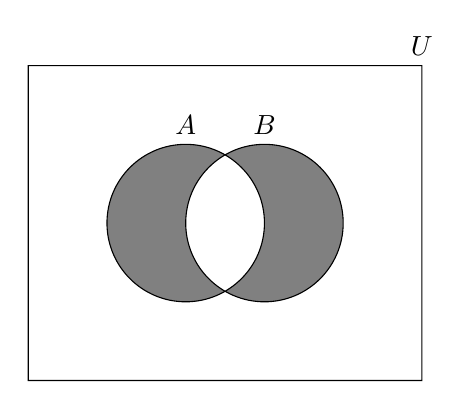
\begin{tikzpicture}[fill=gray]
                \scope
                \clip (-2,-2) rectangle (2,2)
                      (1,0) circle (1);
                \fill (0,0) circle (1);
                \endscope
                \scope
                \clip (-2,-2) rectangle (2,2)
                      (0,0) circle (1);
                \fill (1,0) circle (1);
                \endscope
                \draw (0,0) circle (1) (0,1)  node [text=black,above] {$A$}
                      (1,0) circle (1) (1,1)  node [text=black,above] {$B$}
                      (-2,-2) rectangle (3,2) node [text=black,above] {$U$};
            \end{tikzpicture}
        \end{center}
    \end{frameddefn}

    \begin{framedprop}[label={prop diff simm}]{Differenza simmetrica vuota}
        Dati due insiemi $A$ e $B$, si ha che $$A \ \Delta \ B = \varnothing \iff A = B$$
    \end{framedprop}

    \proofiff{
        Per assurdo, sia $A \ \Delta \ B = \varnothing$ e $A \neq B$; si noti che $A \neq B$ se e solo se esiste $x \in A - B$, oppure $x \in B - A$, e dunque

        \begin{itemize}
            \item $x \in A - B \implies x \in A \land x \notin B \implies x \in A \cap \overline B \implies A \ \Delta \ B \neq \varnothing$ $\lightning$
            \item $x \in B - A \implies x \in B \land x \notin A \implies x \in \overline A \cap B \implies A \ \Delta \ B \neq \varnothing$ $\lightning$
        \end{itemize}
    }{
        Per dimostrare la tesi, è sufficiente considerare che $$A = B \implies A \cap \overline B = \overline A \cap B = \varnothing \implies A \ \Delta \ B = \varnothing$$
    }

    \begin{framedthm}{Decidibilità di $EQ_\DFA$}
        $EQ_\DFA$ è decidibile; in simboli $$EQ_\DFA := \{\abk{A, B} \mid A, B \in \DFA : L(A) = L(B) \} \in \DEC$$
    \end{framedthm}

    \begin{proof}
        Sia $M$ una macchina di Turing; una volta controllata la validità della codifica in input, $M$ può convertire i due \DFA $A$ e $B$ forniti in input in un terzo \DFA $C$ --- utilizzando gli algoritmi presentati all'interno della \cref{closure unione}, della \cref{closure inters} e della \cref{closure compl} --- tale che $$L(C) = L(A) \ \Delta \ L(B)$$ e dunque per la \cref{prop diff simm}, si ha che $$L(A) = L(B) \iff L(C) = \varnothing$$ Sia $M'$ la \TM costruita all'interno del \cref{dec e_dfa}; allora, $M$ può utilizzare $M'$ sull'input $\abk{C}$, poiché se $M'$ accetta, allora $L(C) = \varnothing$, e dunque $A$ è equivalente a $B$; allora $M$ accetta se e solo se $M'$ accetta, e poiché $M'$ è decisore per la dimostrazione del \cref{dec e_dfa} stessa, segue la tesi.
    \end{proof}

    \begin{framedthm}{Indecidibilità di $EQ_\CFG$}
        $EQ_\CFG$ è indecidibile; in simboli $$EQ_\CFG := \{\abk{G,H} \mid G,H \in \CFG : L(G) = L(H)\} \notin \DEC$$
    \end{framedthm}

    \begin{proof}
        Omessa.
    \end{proof}

    \chapter{Riducibilità}

    \section{Riduzione}

    \subsection{Funzioni calcolabili}

    \begin{frameddefn}{Riduzione}
        Una \tbf{riduzione} è un modo di convertire un problema in un altro, in modo tale che una soluzione al secondo possa essere utilizzata per risolvere il primo.
    \end{frameddefn}

    \begin{frameddefn}{Funzione calcolabile}
        Una funzione $\func{f}{\Sigma^*}{\Sigma^*}$ è detta \tbf{funzione calcolabile} se esiste una macchina di Turing che, su qualsiasi input $w \in \Sigma^*$, se si ferma, termina avendo solo $f(w)$ sul suo nastro.
    \end{frameddefn}

    \begin{frameddefn}{Riduzione mediante funzione}
        Siano $A$ e $B$ due linguaggi definiti su un alfabeto $\Sigma$; $A$ è detto essere \tbf{riducibile mediante funzione a $B$} se esiste una funzione calcolabile $\func{f}{\Sigma^*}{\Sigma^*}$ tale che $$\forall w \in \Sigma^* \quad w \in A \iff f(w) \in B$$ Tale relazione è indicata attraverso il simbolismo $$A \leq_\mathrm m B$$ e la funzione $f$ prende il nome di \tbf{riduzione di $A$ a $B$}.
    \end{frameddefn}

    \begin{framedlem}[label={red compl}]{Riducibilità dei complementi}
        Siano $A$ e $B$ due linguaggi definiti su un alfabeto $\Sigma$; allora, si ha che $$A \leq_\mathrm m B \iff \overline A \leq_\mathrm m \overline B$$
    \end{framedlem}

    \begin{proof}
        Si assuma $A \leq_\mathrm m B$, senza perdita di generalità; allora, per definizione, esiste una funzione calcolabile $\func{f}{\Sigma^*}{\Sigma^*}$ tale che $\forall w \in \Sigma ^* \quad w \in A \iff f(w) \in B$. Allora, si ha che $$w \in \overline A \iff w \notin A \iff f(w) \notin B \iff f(w) \in \overline B$$ e dunque $f$, poiché calcolabile, è anche la riduzione da $\overline A$ a $\overline B$, dunque per definizione segue che $\overline A \leq_\mathrm m \overline B$.
    \end{proof}

    \begin{framedlem}[label={red trans}]{Transitività della riducibilità}
        Siano $A$, $B$ e $C$ tre linguaggi definiti su un alfabeto $\Sigma$; allora, si ha che $$\soe{l}{A \leq_\mathrm m B \\ B \leq_\mathrm m C} \implies A \leq_\mathrm m C$$
    \end{framedlem}

    \begin{proof}
        Per definizione stessa, poiché $A \leq_\mathrm m B$ e $B \leq_\mathrm m C$, esistono funzioni calcolabili $\func{f, g}{\Sigma^*}{\Sigma^*}$ tali che $$\centeredsoe{\forall w \in \Sigma ^* \quad w \in A \iff f(w) \in B \\ \forall w \in \Sigma^* \quad w \in B \iff g(w) \in C}$$ dunque, segue che $$\forall w \in \Sigma^* \quad w \in A \iff f(w) \in B \iff g(f(w)) \in C$$ ed è quindi possibile definire una funzione $F := (g \circ f)$ tale che $$\forall w \in \Sigma^* \quad w \in A \iff F(w) \in C$$ Si consideri infine la seguente macchina di Turing $M$ che, data in input una stringa $w$, computa come segue:

        \begin{itemize}
            \item $M$ calcola $f(w)$ attraverso la \TM che rende $f$ calcolabile;
            \item $M$ calcola $g(f(w))$ attraverso la \TM che rende $g$ calcolabile;
            \item $M$ restituisce $g(f(w))$ sul proprio nastro.
        \end{itemize}

        Allora, per costruzione di $M$, se $M$ si ferma, termina avendo solo $F(w) = g(f(w))$ sul suo nastro; di conseguenza, $F$ risulta essere una funzione calcolabile, per le proprietà di $F$ precedentemente discusse, segue la tesi.
    \end{proof}

    \section{Turing-decidibilità mediante riduzione}

    \subsection{Teoremi}

    \begin{framedthm}[label={dec w red}]{Decidibilità mediante riduzione}
        Siano $A$ e $B$ due linguaggi definiti su un alfabeto $\Sigma$; se $A \leq_\mathrm m B$, e $B$ è decidibile, allora $A$ è decidibile. In simboli $$\soe{l}{A \leq_\mathrm m B \\ B \in \DEC} \implies A \in \DEC$$
    \end{framedthm}

    \begin{proof}
        Poiché $B \in \DEC$ in ipotesi, esiste un decisore $M$ tale che $M$ decide $B$; inoltre, poichè $A \leq_\mathrm m B$, esiste una funzione calcolabile $\func{f}{\Sigma^*}{\Sigma^*}$ tale per cui $A$ sia riducibile a $B$. Sia dunque $N$ una macchina di Turing che, data in input una stringa $w \in \Sigma^*$, computa come segue:

        \begin{itemize}
            \item $N$ computa $f(w)$ attraverso la \TM che rende $f$ calcolabile;
            \item $N$ simula $M$ avente $f(w)$ come input; 
            \item $N$ accetta se e solo se $M$ accetta.
        \end{itemize}

        Allora, per costruzione di $N$, e per riducibilità di $A$ a $B$, si ha che $$w \in L(N) \iff f(w) \in L(M) = B \iff w \in A$$ e dunque $N$ decide $A$.
    \end{proof}

    \begin{framedcor}[label={dec w red cor}]{Indecidibilità mediante riduzione}
        Siano $A$ e $B$ due linguaggi definiti su un alfabeto $\Sigma$; se $A \leq_\mathrm m B$, ed $A$ è indecidibile, allora $B$ è indecidibile. In simboli $$\soe{l}{A \leq_\mathrm m B \\ A \notin \DEC} \implies B \notin \DEC$$
    \end{framedcor}

    \begin{proof}
        Per assurdo, sia $B \in \DEC$; allora, poiché $A \leq_\mathrm m B$, per il \cref{dec w red}, si ha che $A \in \DEC$ $\lightning$.
    \end{proof}

    \subsection{Problema della terminazione}

    \begin{frameddefn}{Linguaggi di terminazione}
        Si definiscono \tbf{linguaggi di terminazione} i linguaggi definiti come segue $$HALT_\mathcal{C} := \{\abk{A, w} \mid A \in \mathcal{C} , A \ \textrm{si ferma su input} \ w\}$$
    \end{frameddefn}

    \begin{framedthm}{Indecidibilità di $HALT_\TM$}
        $HALT_\TM$ è indecidibile; in simboli $$HALT_\TM := \{\abk{M, w} \mid M \in \TM , M \ \textrm{si ferma su input} \ w\} \notin \DEC$$
    \end{framedthm}

    \begin{proof}[Dimostrazione I]
        Per assurdo, sia $HALT_\TM$ decidibile, e dunque per esso esiste un decisore $H$; di conseguenza $H(\abk{M, w})$ accetta se e solo se $M$ si ferma avendo $w$ come input. Si consideri ora una macchina di Turing $D$ --- avente $H$ come sua sottoprocedura --- che, data in input una codifica $\abk{M, w}$, computa come segue:

        \begin{itemize}
            \item $D$ esegue $H(\abk{M,w})$;
            \item se $H$ rifiuta, allora $M$ va in loop avendo $w$ come input, e dunque $D$ rifiuta;
            \item se $H$ accetta, allora $M$ si ferma avendo $w$ come input, e dunque $D$ procede a simulare $M$ stessa:
            \begin{itemize}
                \item se $M$ accetta, $D$ accetta
                \item se $M$ rifiuta, $D$ rifiuta.
            \end{itemize}
        \end{itemize}

        Di conseguenza, $D$ è in grado di stabilire, data una macchina di Turing $M$ ed un input $w$, se $w \in L(M)$; inoltre, si noti che $D$ non può andare in loop, e dunque $D$ è un decisore. Allora, l'esistenza di $D$ dimostrerebbe che $A_\TM \in \DEC$, ma questo è assurdo per il \cref{a_tm not in dec} $\lightning$.
    \end{proof}

    \begin{proof}[Dimostrazione II]
        Si consideri la macchina di Turing $F$ che, data in input una codifica $\abk{M, w}$, computa come segue:

        \begin{itemize}
            \item $F$ costruisce una macchina di Turing $M'$ che, data in input una stringa $x$, computa come segue:
                \begin{itemize}
                    \item $M'$ esegue $M(x)$
                    \item se $M$ accetta, $M'$ accetta;
                    \item se $M$ rifiuta, $M'$ cicla (ad esempio muovendo la testina verso una direzione per sempre);
                \end{itemize}
            \item $F$ restituisce $\abk{M', w}$ sul suo nastro.
        \end{itemize}

        Si noti dunque che, poiché $F$ si ferma avendo solo $\abk{M', w}$ sul nastro, per qualsiasi input $\abk{M, w}$, la funzione $\funcmap{f}{\Sigma^*}{\Sigma^*}{\abk{M, w}}{\abk{M', w}}$ che $F$ descrive è calcolabile per definizione. Allora, si noti che $$\abk{M, w} \in A_\TM \iff w \in L(M) \iff w \in L(M')$$ per definizione di $A_\TM$ e per costruzione di $M'$ rispettivamente; inoltre $$w \in L(M') \iff f(\abk{M, w}) = \abk{M', w} \in HALT_\TM$$ per definizione di $HALT_\TM$; dunque $$\abk{M, w} \in A_\TM \iff f(\abk{M, w}) \in HALT_\TM$$ Allora, per definizione, segue che $$A_\TM \leq_\mathrm m HALT_\TM$$ e poiché $A_\TM \notin \DEC$ per il \cref{a_tm not in dec}, è verificata la tesi per cui $HALT_\TM \notin \DEC$ per il \cref{dec w red cor}.
    \end{proof}

    \subsection{Problema del vuoto}

    \begin{framedthm}[label={e_tm not in dec}]{Indecidibilità di $E_\TM$}
        $E_\TM$ è indecidibile; in simboli $$E_\TM := \{\abk{M} \mid M \in \TM : L(M) = \varnothing \} \notin \DEC$$
    \end{framedthm}

    \begin{proof}
        Per assurdo, sia $E_\TM$ decidibile, e dunque per esso esiste un decisore $H$; di conseguenza $H(\abk{M})$ accetta se e solo se $L(M) = \varnothing$. Si consideri ora una macchina di Turing $D$ --- avente $H$ come sua sottoprocedura --- che, data in input una codifica $\abk{M, w}$, computa come segue:

        \begin{itemize}
            \item $D$ costruisce una macchina di Turing $M'$ che, data in input una stringa $x$, computa come segue:
                \begin{itemize}
                    \item se l'input $x$ di $M$ è proprio $w$, $M'$ accetta se $M$ accetta;
                    \item se l'input $x$ di $M$ non è $w$, $M'$ rifiuta;
                \end{itemize}
                (si noti che questa macchina è realizzabile poiché è sufficiente aggiungere ad $M$ degli stati che controllano l'input fornito, e computare come descritto);
            \item $D$ esegue $H(\abk{M'})$;
            \item se $H$ accetta, allora $L(M') = \varnothing$, e dunque $D$ rifiuta;
            \item se $H$ rifiuta, allora $L(M') \neq \varnothing$, e dunque $D$ accetta.
        \end{itemize}

        Di conseguenza, $D$ è in grado di stabilire, data una macchina di Turing $M$ ed un input $w$, se $w \in L(M)$, poiché accetta se e solo se $H$ rifiuta, ovvero se e solo se $L(M') \neq \varnothing$, e per costruzione di $M'$ si ha che $L(M') \neq \varnothing \iff L(M') = \{ w\}$; inoltre, si noti che $D$ non può andare in loop, e dunque $D$ è un decisore. Allora, l'esistenza di $D$ dimostrerebbe che $A_\TM \in \DEC$, ma questo non è possibile per il \cref{a_tm not in dec} $\lightning$.
    \end{proof}

    \subsection{Problema della regolarità}

    \begin{frameddefn}{Linguaggi di regolarità}
        Si definiscono \tbf{linguaggi di regolarità} i linguaggi definiti come segue $$REG_\mathcal{C} := \{\abk{A} \mid A \in \mathcal{C} , L(A) \in \REG\}$$
    \end{frameddefn}

    \begin{framedthm}{Indecidibilità di $REG_\TM$}
        $REG_\TM$ è indecidibile; in simboli $$REG_\TM := \{\abk{M} \mid M \in \TM , L(M) \in \REG\} \notin \DEC$$
    \end{framedthm}

    \begin{proof}
        Per assurdo, sia $REG_\TM$ decidibile, e dunque per esso esiste un decisore $H$; di conseguenza $H(\abk{M})$ accetta se e solo se $L(M) \in \REG$. Si consideri ora una macchina di Turing $D$ --- avente $H$ come sua sottoprocedura --- che, data in input una codifica $\abk{M, w}$, computa come segue:

        \begin{itemize}
            \item $D$ costruisce una macchina di Turing $M'$ che, data in input una stringa $x$, computa come segue:
                \begin{itemize}
                    \item se l'input $x$ di $M'$ ha la forma $\ttt 0^n \ttt 1 ^n$ (per qualche $n \in \N$), $M'$ accetta;
                    \item se l'input $x$ di $M'$ non ha tale forma, $M'$ accetta se $M(w)$ accetta (dunque ignorando $x$);
                \end{itemize}
            \item $D$ esegue $H(\abk{M'})$;
            \item se $H$ accetta, allora $L(M') \in \REG$, e dunque $D$ accetta;
            \item se $H$ rifiuta, allora $L(M') \in \REG$, e dunque $D$ rifiuta.
        \end{itemize}

        Di conseguenza, $D$ è in grado di stabilire, data una macchina di Turing $M$ ed un input $w$, se $w \in L(M)$, poiché accetta se e solo se $H$ accetta, ovvero se $L(M') \in \REG$, e per costruzione di $M'$ si ha che $L(M') \in \REG \iff \soe{l}{x \notin \{\ttt 0 ^n \ttt 1 ^n \mid n \in \N\} \\ M(w) \ \textrm{accetta}}$ TODO DA FINIRE NON HO CAPITO
    \end{proof}

    \subsection{Problema dell'uguaglianza}

    \begin{framedthm}{Indecidibilità di $EQ_\TM$}
        $EQ_\TM$ è indecidibile; in simboli $$EQ_\TM := \{\abk{M_1, M_2} \mid M_1, M_2 \in \TM, L(M_1) = L(M_2)\} \notin \DEC$$
    \end{framedthm}

    \begin{proof}[Dimostrazione I]
        Per assurdo, sia $EQ_\TM$ decidibile, e dunque per esso esiste un decisore $H$; di conseguenza $H(\abk{M_1}, {M_2})$ accetta se e solo se $L(M_1)= L(M_2)$. Si consideri ora una macchina di Turing $D$ --- avente $H$ come sua sottoprocedura --- che, data in input una codifica $\abk{M}$, computa come segue:

        \begin{itemize}
            \item $D$ esegue $H(\abk{M, M_\mathrm{reject}})$, dove $M_\mathrm{reject }$ è una macchina di Turing che rifiuta ogni input, e dunque $L(M_\mathrm{reject}) = \varnothing$;
            \item se $H$ accetta, allora $L(M) = L(M_\mathrm{reject}) = \varnothing$, e dunque $D$ accetta;
            \item se $H$ rifiuta, allora $L(M) \neq L(M_\mathrm{reject}) = \varnothing$, e dunque $D$ rifiuta.
        \end{itemize}

        Di conseguenza, $D$ è in grado di stabilire, data una macchina di Turing $M$, se $L(M) = \varnothing$, poiché attraverso $H$ controlla che il linguaggio di $M$ coincida con $L(M_\mathrm{reject})= \varnothing$; inoltre, si noti che $D$ non può andare in loop, e dunque $D$ è un decisore. Allora, l'esistenza di $D$ dimostrerebbe che $E_\TM \in \DEC$, ma questo non è possibile per il \cref{e_tm not in dec} $\lightning$.
    \end{proof}

    \begin{proof}[Dimostrazione II]
        Si consideri la macchina di Turing $F$ che, data in input una codifica $\abk{M}$, computa come segue:

        \begin{itemize}
            \item $F$ costruisce una macchina di Turing $M'$ che, data in input una stringa $x$, rifiuta sempre --- e dunque $L(M') = \varnothing$;
            \item $F$ restituisce $\abk{M, M'}$ sul suo nastro.
        \end{itemize}
        
        Si noti dunque che, poiché $F$ si ferma avendo solo $\abk{M, M'}$ sul natro, per qualsiasi input $\abk{M}$, la funzione $\funcmap{f}{\Sigma^*}{\Sigma^*}{\abk{M}}{\abk{M, M'}}$ che $F$ descrive è calcolabile per definizione. Allora, si noti che $$\abk{M} \in E_\TM \iff L(M) = \varnothing = L(M')$$ per definizione di $E_\TM$ e per costruzione di $M'$ rispettivamente; inoltre $$L(M') = L(M) \iff f(\abk{M}) = \abk{M, M'} \in EQ_\TM$$ per definizione di $EQ_\TM$; dunque $$\abk{M} \in E_\TM \iff f(\abk{M}) \in EQ_\TM $$ Allora, per definizione, segue che $$E_\TM \leq_\mathrm m EQ_\TM$$ e poiché $E_\TM \notin \DEC$ per il \cref{e_tm not in dec}, è verificata la tesi per cui $EQ_\TM \notin \DEC$ per il \cref{dec w red cor}.
    \end{proof}

    \section{Turing-riconoscibilità mediante riduzione}

    \subsection{Teoremi}

    \begin{framedthm}[label={rec w red}]{Turing-riconoscibilità mediante riduzione}
        Siano $A$ e $B$ due linguaggi definiti su un alfabeto $\Sigma$; se $A \leq_\mathrm m B$, e $B$ è Turing-riconoscibile, allora $A$ è Turing-riconoscibile. In simboli $$\soe{l}{A \leq_\mathrm m B \\ B \in \REC} \implies A \in \REC$$
    \end{framedthm}

    \begin{proof}
        La dimostrazione è analoga alla dimostrazione del \cref{dec w red}, tranne per il fatto che le macchine di Turing considerate sono riconoscitori e non decisori; verrà dunque omessa.
    \end{proof}

    \begin{framedcor}[label={rec w red cor}]{Turing-irriconoscibilità mediante riduzione}
        Siano $A$ e $B$ due linguaggi definiti su un alfabeto $\Sigma$; se $A \leq_\mathrm m B$, ed $A$ non è Turing-riconoscibile, allora $B$ non è Turing-riconoscibile. In simboli $$\soe{l}{A \leq_\mathrm m B \\ A \notin \REC} \implies B \notin \REC$$
    \end{framedcor}

    \begin{proof}
        Per assurdo, sia $B \in \REC$; allora, poiché $A \leq_\mathrm m B$, per il \cref{rec w red} si ha che $A \in \REC$ $\lightning$.
    \end{proof}

    \begin{framedcor}[label={corec w red}]{Co-riconoscibilità mediante riduzione}
        Siano $A$ e $B$ due linguaggi definiti su un alfabeto $\Sigma$; se $A \leq_\mathrm m B$, ed $B$ è co-Turing-riconoscibile, allora $A$ è co-Turing-riconoscibile. In simboli $$\soe{l}{A \leq_\mathrm m B \\ B \in \coREC} \implies A \in \coREC$$
    \end{framedcor}

    \begin{proof}
        Per il \cref{red compl} si ha che $$A \leq_\mathrm m B \iff \overline{A} \leq_\mathrm m \overline B$$ e dunque, per il \cref{rec w red}, si ha che $$\soe{l}{\overline A \leq_\mathrm m \overline B \\ B \in \coREC \iff \overline B \in \REC} \implies \overline A \in \REC \iff A \in \coREC$$ 
    \end{proof}

    \begin{framedcor}[label={corec w red cor}]{Co-irriconoscibilità mediante riduzione}
        Siano $A$ e $B$ due linguaggi definiti su un alfabeto $\Sigma$; se $A \leq_\mathrm m B$, ed $A$ non è co-Turing-riconoscibile, allora $B$ è non co-Turing-riconoscibile. In simboli $$\soe{l}{A \leq_\mathrm m B \\ A \notin \coREC} \implies B \notin \coREC$$
    \end{framedcor}

    \begin{proof}
        Per assurdo, sia $B \in \coREC$; allora, poiché $A \leq_\mathrm m B$, per il \cref{corec w red}, si ha che $A \in \coREC$ $\lightning$.
    \end{proof}

    \begin{framedcor}{Riducibilità al proprio complemento}
        Sia $A$ un linguaggio tale da essere riducibile al suo complemento; allora, se $A$ è Turing-riconoscibile, è anche decidibile. In simboli $$\soe{l}{A \leq_\mathrm m \overline A \\ A \in \REC} \implies A \in \DEC$$
    \end{framedcor}

    \begin{proof}
        Per il \cref{red compl} si ha che $$A \leq_\mathrm m \overline A \iff \overline A \leq_\mathrm m \overline {\overline A} = A$$ e dunque, per il \cref{rec w red}, si ha che $$\soe{l}{\overline A \leq_\mathrm m A \\ A \in \REC} \implies \overline A \in \REC \iff A \in \coREC$$ e poiché $$\DEC = \REC \cap \coREC$$ per il \cref{coturing thm}, segue che $A \in \DEC$.
    \end{proof}

    \subsection{Problema dell'uguaglianza}

    \begin{framedthm}[label={eq_tm not in rec}]{Irriconoscibilità di $EQ_\TM$}
        $EQ_\TM$ non è Turing-riconoscibile; in simboli $$EQ_\TM := \{\abk{M_1, M_2} \mid M_1, M_2 \in \TM, L(M_1) = L(M_2)\} \notin \REC$$
    \end{framedthm}

    \begin{proof}
        Si consideri la macchina di Turing $F$ che, data in input una codifica $\abk{M, w}$, computa come segue:

        \begin{itemize}
            \item $F$ costruisce una macchina di Turing $M_1$ che, data in input una stringa $x$, rifiuta sempre --- e dunque $L(M_1) = \varnothing$;
            \item $F$ costruisce una macchina di Turing $M_2$ che, data in input una stringa $x$, computa come segue:
                \begin{itemize}
                    \item $M_2$ esegue $M(w)$ (dunque ignorando $x$);
                    \item se $M$ accetta, $M_2$ accetta;
                    \item se $M$ rifiuta o cicla, $M_2$ rifiuta;
                \end{itemize}
                dunque, se $M$ accetta $w$, $M_2$ riconosce $\Sigma^*$, altrimenti $M_2$ riconosce $\varnothing$;
            \item $F$ restituisce $\abk{M_1, M_2}$ sul suo nastro.
        \end{itemize}

        Si noti dunque che, poiché $F$ si ferma avendo solo $\abk{M_1, M_2}$ sul nastro, per qualsiasi input $\abk{M, w}$, la funzione $\funcmap{f}{\Sigma^*}{\Sigma^*}{\abk{M, w}}{\abk{M_1, M_2}}$ che $F$ descrive è calcolabile per definizione. Allora, si noti che $$\abk{M, w} \in A_\TM \iff w \in L(M) \iff L(M_2) = \Sigma ^*$$ per definizione di $A_\TM$ e per costruzione di $M_2$ rispettivamente; inoltre $$L(M_1) = \varnothing \neq L(M_2) \iff f(\abk{M, w}) = \abk{M_1, M_2} \notin EQ_\TM \iff \abk{M_1, M_2} \in \overline{EQ_\TM}$$ per definizione di $EQ_\TM$; dunque $$\abk{M, w} \in A_\TM \iff f(\abk{M, w}) \in \overline{EQ_\TM}$$ Allora, per definizione, segue che $$A_\TM \leq_\mathrm m \overline{EQ_\TM}$$ e poiché $A_\TM \notin \coREC$ per il \cref{a_tm not in corec}, è verificata la tesi per cui $\overline{EQ_\TM} \notin \coREC \iff EQ_\TM \notin \REC$, per il \cref{corec w red cor}.
    \end{proof}

    \begin{framedthm}{Irriconoscibilità di $\overline{EQ_\TM}$}
        $EQ_\TM$ non è co-Turing-riconoscibile; in simboli $$EQ_\TM := \{\abk{M_1, M_2} \mid M_1, M_2 \in \TM, L(M_1) = L(M_2)\} \notin \coREC$$
    \end{framedthm}

    \begin{proof}
        Si consideri la dimostrazione del \cref{eq_tm not in rec}; in essa, la \TM $F$ costruisce due macchine di Turing $M_1$ ed $M_2$, dove la prima riconosce $\varnothing$. Se $M_1$ fosse invece tale da accettare sempre, riconoscerebbe $\Sigma^*$, e dunque si avrebbe che $$\abk{M, w} \in A_\TM \iff w \in L(M) \iff L(M_2) = \Sigma^*$$ per definizione di $A_\TM$ e per costruzione di $M_2$ rispettivamente; inoltre $$L(M_1)=L(M_2) \iff f(\abk{M, w}) = \abk{M_1, M_2} \in EQ_\TM$$ per definizione di $EQ_\TM$; dunque $$\abk{M, w} \in A_\TM \iff f(\abk{M, w}) \in EQ_\TM$$ Allora, per definizione, segue $$A_\TM \leq_\mathrm m EQ_\TM$$ e poiché $A_\TM \notin \coREC$ per il \cref{a_tm not in corec}, è verificata la tesi per cui $EQ_\TM \notin \REC$, per il \cref{corec w red cor}.
    \end{proof}

    \chapter{Complessità di tempo}

    \section{Analisi asintotica}
    
    \subsection{$O$-grande ed $o$-piccolo}

    \begin{frameddefn}{$O$-grande}
        Siano $\func{f, g}{\N}{\R^+}$; $f(n)$ è detta essere \tbf{in $O$-grande di $g(n)$} se e solo se $$\exists c \in \R_{>0}, n_0 \in \N_{>0} \mid \forall n \ge n_0 \quad f(n) \leq c \cdot g(n)$$ ed è indicato con il simbolismo $$f(n) = O(g(n))$$ Viceversa, $g(n)$ è detto essere \tbf{limite superiore asintotico} per $f(n)$.
    \end{frameddefn}

    \begin{example}[$O$-grande]
        \label{big o ex}
        Siano $f(n) = 100 n^2$ e $g(n) = n^3$; poiché esistono $c = 10$ ed $n_0 = 10$ tali che $$\forall n \ge n_0 = 10 \quad f(n) = 100 n^2 \leq 10 \cdot n^3 = c \cdot g(n)$$ si ha che $f(n) = O(g(n))$ per definizione.
    \end{example}

    \begin{frameddefn}{$o$-piccolo}
        Siano $\func{f, g}{\N}{\R^+}$; $f(n)$ è detta essere \tbf{in $o$-piccolo di $g(n)$} se e solo se $$\lim_{n \to + \infty}{\dfrac{f(n)}{g(n)}} = 0$$ o equivalentemente, se e solo se $$\exists c \in \R_{> 0}, n_0 \in \N_{>0} \mid \forall n \ge n_0 \quad f(n) < c \cdot g(n)$$ ed è indicato con il simbolismo $$f(n) = o(g(n))$$
    \end{frameddefn}

    \begin{example}[$o$-piccolo]
        Si consideri l'\cref{big o ex}; poiché sono stati scelti $c = n_0 = 10$, per $n = n_0$ si ottiene che $$f(n_0) = f(10) = 100 \cdot 10^2 = 10000 = 10 \cdot 1000 = 10 \cdot 10^3 = 10 \cdot g(10) = c \cdot g(n_0)$$ Allora, scegliendo $n_0$ tale da essere maggiore di 10 --- dunque ad esempio 11 --- si ha che $$\forall n \ge n_0 = 11 \quad f(n) = 100 n^2 < 10 \cdot n^3 = c \cdot g(n)$$ e dunque $f(n) = o(g(n))$ per definizione.
    \end{example}

    \begin{framedobs}[label={small o big o obs}]{$O$-grande ed $o$-piccolo}
        Si noti che, date due funzioni $\func{f,g}{\N}{\R^+}$, per definizione stessa si ha che $$f(n) = o(g(n)) \implies f(n)= O(g(n))$$
    \end{framedobs}

    \begin{framedprop}[label={alg asintotica}]{Algebra asintotica}
        Siano $\func{f, g, h}{\N}{\R^+}$; allora, si ha che:
        
        \begin{itemize}
            \item $\forall c \in \R \quad f(n) = c \cdot o(g(n)) \implies f(n) = o(g(n))$
            \item $f(n) = o(g(n)) + o(h(n)) \implies f(n) = o(\max(g(n), h(n)))$
            \item $f(n) = o(g(n)) \cdot o(h(n)) \implies f(n) = o(g(n) \cdot h(n))$
        \end{itemize}

        Si noti che tali regole valgono anche per $O$-grande, per l'\cref{small o big o obs}.
    \end{framedprop}

    \begin{framedobs}[label={fn log}]{Funzioni logaritmiche}
        Per convenzione, le funzioni logaritmiche si esprimono in termini di $\log_2$, ed è possibile farlo grazie alle proprietà dei logaritmi, infatti $$\forall k \in \R \quad f(n) = \log_k(n) \implies f(n) = O(\log_k(n)) = O \rbk{\dfrac{\log_2(n)}{\log_2(k)}} = O(\log_2(n))$$
    \end{framedobs}

    \begin{framedobs}[label={fn exp}]{Funzioni esponenziali}
        Per convenzione, le funzioni esponenziali si esprimono in termini di potenze di 2, ed è possibile farlo grazie alle proprietà delle potenze, infatti $$\forall k \in \R \quad f(n) = k^n = 2^{\log_2\rbk{k^n}} = 2^{n \cdot \log_2 (k)} = 2^{O(n)}$$

        Inoltre, una funzione $f(n) = O\rbk{2^{O(n)}}$, per definizione, ha come limite superiore asintotico $2^{O(n)}$, ed è dunque superata asintoticamente da una funzione $c \cdot 2^{O(n)}$ per qualche $c \in \N - \{0\}$; allora, per proprietà delle potenze, si ha che $$c \cdot 2^{O(n)} = 2^{\log_2(c)} \cdot 2^{O(n)} = 2^{\log_2(c) + O(n)} = 2^{O(n)}$$ implicando che $f(n) = O\rbk{2^{O(n)}} = 2^{O(n)}$.
    \end{framedobs}

    \begin{framedprop}[label={o trans}]{Transitività di $o$-piccolo}
        Siano $\func{f, g, h}{\N}{\R^+}$; allora, si verifica che $$\soe{l}{f(n) = o(g(n)) \\ g(n) = o(h(n))} \implies f(n) = o(h(n))$$
    \end{framedprop}

    \begin{proof}
        Per definizione, si ha che $$f(n) = o(g(n)) \iff \displaystyle \lim_{n \to + \infty}{\dfrac{f(n)}{g(n)} = 0}$$ e che $$g(n) = o(h(n)) \iff \displaystyle \lim_{n \to + \infty}{\dfrac{g(n)}{h(n)}} = 0$$ allora, segue che $$\lim_{n \to + \infty}{\dfrac{f(n)}{h(n)}} = \lim_{n \to + \infty}{\dfrac{f(n)}{g(n)} \cdot \dfrac{g(n)}{h(n)}} = 0 \iff f(n) = o(h(n))$$
    \end{proof}

    \section{Complessità di tempo di macchine di Turing}

    \subsection{Macchine di Turing}

    \begin{frameddefn}{Complessità di tempo di una \TM}
        Sia $D$ un decisore; si definisce \tbf{complessità di tempo} (o \tbf{tempo di esecuzione}) di $D$ la funzione $\func{f}{\N}{\N}$ tale che $f(n)$ sia il numero massimo di passi che $D$ utilizza per processare una stringa di lunghezza $n$.
    \end{frameddefn}

    \begin{example}[Complessità di tempo di \TM]
        Sia $D$ un decisore che, data in input una stringa $x$, sposta la testina verso destra finché non legge $\blankchar$, e quando legge quest'ultimo accetta. Allora, se input è presente una stringa avente lunghezza $n$, $D$ impiega esattamente $n$ passi a processarla, e dunque $f(n) = n \implies f \equiv \id$.
    \end{example}

    \subsection{Macchine di Turing multinastro}

    \begin{framedthm}{Relazione tra \TM e \TM multinastro}
        Sia $t(n)$ una funzione tale che $t(n) \ge n$, e sia $M$ una macchina di Turing multinastro avente tempo $t(n)$; allora, esiste una \TM $M'$, equivalente ad $M$, avente tempo $O(t^2(n))$.
    \end{framedthm}

    \begin{proof}
        Sia $M$ una macchina di Turing a $k$-nastri avente tempo di esecuzione $t(n)$, e si consideri la \TM $M'$ costruita all'interno della prima implicazione della dimostrazione della \cref{multitape equiv}. Dunque, si ha che:

        \begin{itemize}
            \item il numero di nastri $k$ non dipende dall'input, ed è dunque costante;
            \item si assuma $n$ essere la lunghezza della stringa più lunga tra le stringhe presenti sui nastri di $M$; allora, per trasformare il nastro nel formato descritto all'interno della dimostrazione --- ovvero effettuando uno \tit{shift} verso destra, anteponendo \ttt \# all'inizio e inserendo i caratteri marcati per segnare le testine virtuali --- sono necessari $O(n) + O(n) + O(n) = O(n)$ passi;
            \item si considerino le parti attive dei nastri di $M$: nel caso peggiore (ovvero se la testina di $M$ non fa altro che spostarsi a destra), ognuna di queste ha lunghezza $t(n)$, poiché $M$ utilizza $t(n)$ celle del nastro in $t(n)$ passi; di conseguenza, una scansione della parte attiva del nastro di $M'$ impiega $k \cdot O(t(n))= O(t(n))$ passi;
            \item per simulare una singola mossa di $M$, la testina di $M'$ scansiona tutto il suo nastro, aggiorna le testina virtuali, e successivamente effettua una seconda scansione per simulare i rimpiazzi; allora, un singolo passo di $M$ impiega $2 \cdot O(t(n)) = O(t(n))$;
            \item allora, poiché il numero di passi da simulare è $t(n)$, la complessità temporale di $M$ risulta essere $$O(n) + t(n) \cdot O(t(n)) = O(t^2(n))$$
        \end{itemize}
    \end{proof}

    \subsection{Macchine di Turing non deterministiche}

    \begin{framedthm}[label={ntm time}]{Relazione tra \TM ed \NTM}
        Sia $t(n)$ una funzione tale che $t(n) \ge n$, e sia $M$ una macchina di Turing non deterministica avente tempo $t(n)$; allora, esiste una \TM $M'$, equivalente ad $M$, avente tempo $2^{O(t(n))}$.
    \end{framedthm}

    \begin{proof}
        TODO
    \end{proof}

    \section{Classi di complessità di tempo}

    \subsection{Classe \DTIME}

    \begin{frameddefn}{Classe \DTIME}
        Data una funzione $\func{t}{\N}{\R^+}$, si definisce \tbf{classe di complessità di tempo $\DTIME(t(n))$} l'insieme dei linguaggi decidibili da una macchina di Turing --- \tit{varianti escluse} --- in $O(t(n))$.
    \end{frameddefn}

    \begin{example}[Classe di complessità di tempo]
        Si consideri una macchina di Turing $M$ --- in grado di decidere $L= \{\ttt 0 ^n \ttt 1 ^n \mid n \in \N\}$ --- che, data in input una stringa $x$, computa come segue: 

        \begin{enumerate}
            \item scorre il nastro: se è presente uno \ttt 0 alla destra di un \ttt 1, rifiuta;
            \item torna all'inizio del nastro;
            \item fintanto che sono presenti almeno uno \ttt 0 ed almeno un \ttt 1, ripete i seguenti passi:
                \begin{enumerate}[label=\arabic*.]
                    \setcounter{enumii}{3}
                    \setcounter{enumi}{6}
                    \item scorre il nastro: se trova uno \ttt 0, lo rimpiazza con \ttt x;
                    \item scorre il nastro: se trova uno \ttt 1, lo rimipazza con \ttt x;
                    \item torna all'inizio del nastro;
                \end{enumerate}
            \item scorre il nastro: se sono presenti solo \ttt x sul nastro, accetta.
        \end{enumerate}

        Se uno qualsiasi dei passaggi menzionati non è effettuabile, $M$ rifiuta; dunque ci si convince facilmente che $M$ decide $L$ come richiesto.

        Analizzando la complessità temporale di $M$, si ottiene che:

        \begin{itemize}
            \item l'istruzione 1 richiede $n$ passi, ed ha dunque costo $O(n)$;
            \item l'istruzione 2 richiede $n$ passi, ed ha dunque costo $O(n)$;
            \item il tempo dell'istruzione 3 dipende dalle istruzioni che ripete, e dunque

                \begin{itemize}
                    \item l'istruzione 4 richiede $n$ passi, ed ha dunque costo $O(n)$;
                    \item analogamente all'istruzione 4, l'istruzione 5 ha costo $O(n)$;
                    \item analogamente all'istruzione 2, l'istruzione 6 ha costo $O(n)$;
                \end{itemize}

                inoltre, si noti che l'istruzione 3 ripete le istruzioni 4, 5 e 6 al più $\dfrac{n}{2}$ volte, poiché ad ogni iterazione vengono rimossi uno \ttt 0 ed un \ttt 1 insieme; allora, per via dei costi delle istruzioni che ripete, l'istruzione 3 ha costo pari a $$\centeredsoe{\dfrac{n}{2} \cdot [O(n) + O(n) + O(n)] = \dfrac{n}{2} \cdot O(\max(n, n, n)) = \\ = \dfrac{n}{2} \cdot O(n) = \dfrac{1}{2} \cdot n \cdot O(n) = \dfrac{1}{2} \cdot O(n \cdot n) = \dfrac{1}{2} \cdot O(n^2) = O(n^2)}$$ (si veda la \cref{alg asintotica});
            \item analogamente all'istruzione 2, l'istruzione 7 ha costo $O(n)$.
        \end{itemize}

        Allora, il costo temporale di $M$ risulta essere $$O(n) + O(n) + O(n^2) + O(n) = O(\max(n, n, n^2, n)) = O(n^2)$$ (si veda la \cref{alg asintotica}) e dunque, segue che $L \in \DTIME \rbk{n^2}$.
    \end{example}

    \subsection{Classe \Pclass}

    \begin{frameddefn}{Classe \Pclass}
        Si definisce \tbf{classe dei linguaggi decidibili in tempo polinomiale} da una \TM a singolo nastro il seguente insieme $$\Pclass := \bigcup_{k \in \N}{\DTIME\rbk{n^k}}$$
    \end{frameddefn}

    \begin{framedobs}{Classe \Pclass}
        La classe di problemi descritti dai linguaggi in \Pclass è particolarmente importante, poiché \Pclass corrisponde approssimativamente alla classe dei problemi che sono realisticamente risolvibili su un computer, in tempi ragionevoli.
    \end{framedobs}

    \begin{frameddefn}{Funzione polinomialmente calcolabile}
        Una funzione $\func{f}{\Sigma^*}{\Sigma^*}$ è detta \tbf{funzione polinomialmente calcolabile} se esiste una macchina di Turing in tempo polinomiale che, su qualsiasi input $w \in \Sigma^*$, se si ferma, termina avendo solo $f(w)$ sul suo nastro.
    \end{frameddefn}

    \begin{frameddefn}{Riduzione polinomiale mediante funzione}
        Siano $A$ e $B$ due linguaggi definiti su un alfabeto $\Sigma$; $A$ è detto essere \tbf{riducibile polinomialmente mediante funzione a $B$} se esiste una funzione polinomialmente calcolabile $\func{f}{\Sigma^*}{\Sigma^*}$ tale che $$\forall w \in \Sigma^* \quad w \in A \iff f(w) \in B$$ Tale relazione è indicata attraverso il simbolismo $$A \leq_\mathrm P B$$ e la funzione $f$ prende il nome di \tbf{riduzione di tempo polinomiale di $A$ a $B$}.
    \end{frameddefn}

    \begin{framedlem}[label={p red compl}]{Riducibilità polinomiale dei complementi}
        Siano $A$ e $B$ due linguaggi definiti su un alfabeto $\Sigma$; allora, si ha che $$A \leq_\mathrm P B \iff \overline A \leq_\mathrm P \overline B$$
    \end{framedlem}

    \begin{proof}
        La dimostrazione è analoga alla dimostrazione del \cref{red compl}, pertanto verrà omessa.
    \end{proof}

    \begin{framedlem}{Transitività della riducibilità polinomiale}
        Siano $A$, $B$ e $C$ tre linguaggi definiti su un alfabeto $\Sigma$; allora, si verifica che $$\soe{l}{A \leq_\mathrm P B \\ B \leq_\mathrm P C} \implies A \leq_\mathrm P C$$
    \end{framedlem}

    \begin{proof}
        La dimostrazione è analoga alla dimostrazione del \cref{red trans}, pertanto verrà omessa.
    \end{proof}

    \begin{framedthm}[label={p w red}]{\Pclass mediante riduzione}
        Siano $A$ e $B$ due linguaggi definiti su un alfabeto $\Sigma$; se $A \leq_\mathrm P B$, e $B$ è in \Pclass, allora $A$ è in \Pclass. In simboli $$\soe{l}{A \leq_\mathrm P B \\ B \in \Pclass} \implies A \in \Pclass$$
    \end{framedthm}

    \begin{proof}
        La dimostrazione è analoga alla dimostrazione del \cref{dec w red}, con la sola differenza che le macchine di Turing considerate computano in tempo polinomiale; verrà dunque omessa.
    \end{proof}

    \begin{framedcor}[label={p with red cor}]{\Pclass mediante riduzione}
        Siano $A$ e $B$ due linguaggi definiti su un alfabeto $\Sigma$; se $A \leq_\mathrm P B$, e $A$ non è in \Pclass, allora $B$ non è in \Pclass. In simboli $$\soe{l}{A \leq_\mathrm P B \\ A \notin \Pclass} \implies B \notin \Pclass$$
    \end{framedcor}

    \begin{proof}
        Per assurdo, sia $B \in \Pclass$; allora, poiché $A \leq_\mathrm P B$, per il \cref{p w red}, si ha che $A \in \Pclass$ $\lightning$.
    \end{proof}

    \begin{framedobs}{Rappresentazione di grafi}
        Nelle prossime dimostrazioni si assumerà che sia possibile definire una codifica coerente per rappresentare grafi $G = (V, E)$, al fine di fornire questi in input a macchine di Turing; un esempio potrebbe essere quello della matrice di adiacenza, in cui la generica cella è definita come segue: $$\forall i, j \in [1, \abs{V}] \quad m_{i, j} = \soe{ll}{1 & (v_i, v_j) \in E \\ 0 & (v_i, v_j) \notin E}$$ dove $v_i, v_j\in V$.
    \end{framedobs}

    \begin{framedthm}[label={path in p}]{$PATH$ in \Pclass}
        Sia $PATH$ il linguaggio definito come segue: $$PATH := \{\abk{G, s, t} \mid G = (V, E) \ \textrm{grafo diretto con un cammino $s \to t$}\}$$ Allora, si verifica che $$PATH \in \Pclass$$
    \end{framedthm}

    \begin{proof}
        Sia $M$ una macchina di Turing che, data in input una codifica $\abk{G, s, t}$, una volta controllata la validità della codifica in input, computa come segue:

        \begin{itemize}
            \item cerca il vertice $s$ tra i vertici di $G$;
            \item una volta trovato, marca $s$;
            \item finche non vengono marcati tutti i vertici di $G$:

                \begin{itemize}
                    \item marca ogni vertice avente un arco entrante da un vertice già marcato;
                \end{itemize}
            \item se tra i vertici marcati è presente $t$, allora $M$ accetta.
        \end{itemize}

        Dunque, poiché $\abs{E}$ è sicuramente minore di $n$ (in quanto il numero di archi è sicuramente inferiore del numero di simboli che servono per rappresentare tutto l'input), sicuramente $\abs{E} = O(n)$, e dunque la complessità temporale di $M$ risulta essere (rispettivamente per ogni istruzione): $$O\rbk{n^k} + O(1) + \abs{E} \cdot O\rbk{n^k} + O\rbk{n^k} = O(n) \cdot O\rbk{n^k} = O(n^{k + 1}) \implies PATH \in \Pclass$$
    \end{proof}

    \subsection{Classe \coPclass}
    
    \begin{frameddefn}{Classe \coPclass}
        La classe \coPclass è definita come segue: $$\coPclass := \{ L \in \DEC \mid \overline L \in \Pclass \}$$
    \end{frameddefn}

    \begin{framedthm}[label={p = cop}]{Relazione tra \Pclass e \coPclass}
        Si verifica che $$\Pclass = \coPclass$$
    \end{framedthm}

    \begin{proof}
        Si consideri un linguaggio $L \in \Pclass$, e dunque per definizione esiste una macchina di Turing $M_L$ che decide $L$ in tempo polinomiale; allora, si consideri la seguente \TM $M_{\overline L}$ che, data in input una stringa $w$, computa come segue:

        \begin{itemize}
            \item $M_{\overline L}$ esegue $M_L(w)$;
            \item $M_{\overline L}$ accetta se e solo se $M_L(w)$ rifiuta.
        \end{itemize}

        Allora, per costruzione, si ha che $$w \in L(M_{\overline L}) \iff w \notin L(M_L) = L$$ e di conseguenza $$L(M_{\overline L}) = \overline L \in \coPclass$$ Inoltre, poiché $M_L$ è un decisore di tempo polinomiale, anche $M_{\overline L}$ è un decisore polinomiale per sua stessa costruzione. Questo dimostra che $\Pclass \subseteq \coPclass$.

        Infine, poiché è possibile ripetere il ragionamento analogo per $\coPclass \subseteq \Pclass$, segue la tesi per doppia implicazione.
    \end{proof}

    \subsection{Classe \EXP}

    \begin{frameddefn}{Classe \EXP}
        Si definisce \tbf{classe dei linguaggi decidibili in tempo esponenziale} da una \TM a singolo nastro il seguente insieme $$\EXP := \bigcup_{k \in N}{\DTIME \rbk{2^{n^k}}}$$
    \end{frameddefn}

    \begin{frameddefn}{Cammino hamiltoniano}
        Sia $G$ un grafo; un \tbf{cammino hamiltoniano} su $G$ è un cammino che passa una sola volta per ogni nodo di $G$.
    \end{frameddefn}

    \begin{framedthm}{$HAMPATH$ in \EXP}
        Sia $HAMPATH$ il linguaggio definito come segue: \centeredeq{0.9}{$HAMPATH := \{\abk{G, s, t} \mid G = (V, E) \ \textrm{grafo diretto con un cammino hamiltoniano $s \to t$}\}$} Allora, si verifica che $$HAMPATH \in \EXP$$
    \end{framedthm}

    \begin{proof}
        Si consideri una macchina di Turing $M$ che, data in input una codifica $\abk{G, s, t}$ in input, computa come segue:

        \begin{itemize}
            \item per ogni possibile cammino $c$ della forma $s \to t$ in $G$, $M$ controlla se $c$ è hamiltoniano; se lo è, $M$ accetta;
            \item se $M$ non ha mai accettato, $M$ rifiuta.
        \end{itemize}

        Allora $M$, per costruzione, è in grado di decidere $HAMPATH$. Si noti che i lnumero di cammini possibili in un grafo è $O \rbk{2^{n^k}}$ per qualche $k \in \N$ --- più precisamente, sarebbe $\displaystyle \rbk{\max_{v \in V}{\deg(v)}}^{O(n)}$ --- e poiché controllare che un cammino sia hamiltoniano richiede tempo $O(n)$, la complessità temporale di $M$ risulta essere $$O(n) \cdot O\rbk{2^{n^k}} = O\rbk{n \cdot 2^{n^k}}$$ e poiché $n^k \ge \log(n)$ (per $k$ sufficientemente grande) si ha che $$O\rbk{n \cdot 2^{n^k}} = O\rbk{2^{n^k}} \implies HAMPATH \in \EXP$$
    \end{proof}

    \subsection{Classe \coEXP}

    \begin{frameddefn}{Classe \coEXP}
        La classe \coEXP è definita come segue: $$\coEXP := \{L \in \DEC \mid \overline A \in \EXP\}$$
    \end{frameddefn}

    \begin{framedthm}[label={exp = coexp}]{Relazione tra \EXP e \coEXP}
        Si verifica che $$\EXP = \coEXP$$
    \end{framedthm}

    \begin{proof}
        La dimostrazione è analoga alla dimostrazione del \cref{p = cop}, pertanto verrà omessa.
    \end{proof}

    \subsection{Classe \NTIME}

    \begin{frameddefn}{Classe \NTIME}
        Data una funzione $\func{t}{\N}{\R^+}$, si definisce \tbf{classe di complessità di tempo $\NTIME(t(n))$} l'insieme dei linguaggi decidibili da una macchina di Turing non deterministica in $O(t(n))$.
    \end{frameddefn}

    \subsection{Classe \NPclass}
    
    \begin{frameddefn}[label={np def}]{Classe \NPclass}
        Si definisce \tbf{classe dei linguaggi decidibili non deterministicamente in tempo polinomiale} da una \NTM il seguente insieme $$\NPclass := \bigcup_{k \in \N}{\NTIME \rbk{n^k}}$$
    \end{frameddefn}

    \begin{framedprop}[label={np exp}]{Tempo polinomiale in \NTIME}
        Si verifica che $$\NPclass \subseteq \EXP$$
    \end{framedprop}

    \begin{proof}
        Sia $L \in \NTIME\rbk{n^k}$ per qualche $k \in \N$, e dunque per definizione esiste una \NTM che decide $L$ in $O\rbk{n^k}$; allora, per il \cref{ntm time}, si ha che $L \in \DTIME \rbk{2^{O\rbk{n^k}}}$.
    \end{proof}

    \begin{framedthm}[label={np w red}]{\NPclass mediante riduzione}
        Siano $A$ e $B$ due linguaggi definiti su un alfabeto $\Sigma$; se $A \leq_\mathrm P B$, e $B$ è in \NPclass, allora $A$ è in \NPclass. In simboli $$\soe{l}{A \leq_\mathrm P B \\ B \in \NPclass} \implies A \in \NPclass$$
    \end{framedthm}

    \begin{proof}
        La dimostrazione è analoga alla dimostrazione del \cref{dec w red}, tranne per il fatto che le macchine di Turing considerate computano non deterministicamente in tempo polinomiale; verrà dunque omessa.
    \end{proof}

    \begin{framedcor}[label={np with red cor}]{\NPclass mediante riduzione}
        Siano $A$ e $B$ due linguaggi definiti su un alfabeto $\Sigma$; se $A \leq_\mathrm P B$, e $A$ non è in \NPclass, allora $B$ non è in \NPclass. In simboli $$\soe{l}{A \leq_\mathrm P B \\ A \notin \NPclass} \implies B \notin \NPclass$$
    \end{framedcor}

    \begin{proof}
        Per assurdo, sia $B \in \NPclass$; allora, poiché $A \leq_\mathrm P B$, per il \cref{np w red}, si ha che $A \in \NPclass$ $\lightning$.
    \end{proof}

    \begin{frameddefn}{Verificatore}
        Sia $L$ un linguaggio decidibile definito su un certo alfabeto $\Sigma$, e $V$ un decisore; $V$ è detto \tbf{verificatore di $L$} se $$L = \{w \in \Sigma^* \mid \exists c \in \Sigma^* : \abk{w, c} \in L(V)\}$$ Data una codifica $\abk{w, c} \in L(V)$, $c$ prende il nome di \tbf{certificato di $w$}.
    \end{frameddefn}

    \begin{framedobs}{Complessità temporale di verificatori}
        Dato un verificatore $V$, ed una codifica $\abk{w, c} \in L(V)$, il tempo di computazione di $V$ è misurato solamente in termini della lunghezza di $w$
    \end{framedobs}

    \begin{frameddefn}{Linguaggio polinomialmente verificabile}
        Un linguaggio è detto essere \tbf{polinomialmente verificabile} se ammette un verificatore in tempo polinomiale.
    \end{frameddefn}

    \begin{framedobs}[label={certif len}]{Certificati di verificatori}
        Sia $V$ un verificatore che computa in $O(f(n))$ per qualche $f$, e sia $\abk{w, c} \in L(V)$; si noti che $c$, per definizione di $V$, può avere qualsiasi lunghezza, ma poiché $V$ deve computare in $O(f(n))$, la porzione di $c$ che verrà utilizzata da parte di $V$ deve comunque essere in $O(f(n))$, poiché $O(f(n))$ è proprio il tempo di cui $V$ dispone per computare.
    \end{framedobs}

    \begin{framedthm}[label={np verif}]{Linguaggi polinomialmente verificabili}
        \NPclass è la classe dei linguaggi polinomialmente verificabili.
    \end{framedthm}

    \proofiff{
        Sia $L \in \NPclass$, e dunque per la \cref{np def} esiste una \NTM $N$ che decide $L = L(N)$ non deterministicamente in tempo polinomiale; sia allora $V$ un decisore che, data in input una configurazione $\abk{w, c}$, computa come segue:

        \begin{itemize}
            \item $V$ interpreta $c$ come un indirizzo (come descritto nella dimostrazione della \cref{ntm tm});
            \item $V$ simula $N$ su input $w$, eseguendo le scelte dettate dall'indirizzo $c$;
            \item $V$ accetta se la simulazione di $N$ accetta.
        \end{itemize}

        Allora, per costruzione di $V$, si ha che $$w \in L = L(N) \iff \exists c \in \Sigma^* \mid \abk{w, c} \in L(V)$$ e, sempre per costruzione di $V$, ciò avviene se e solo se esiste un ramo di $N$ che accetta $w$. Inoltre, poiché $L \in \NPclass$, la lunghezza dei rami dell'albero di computazione di $N$ è necessariamente polinomiale, e dunque se un certificato $c$ descrive una serie di scelte tali che $N$ accetti $w$, la lunghezza di $c$ deve necessariamente essere in polinomiale anch'essa. Di conseguenza, poiché la lunghezza di $c$ determina la computazione di $V$ stessa, $V$ risulta essere un verificatore in tempo polinomiale di $L$.
    }{
        Sia $L$ un linguaggio polinomialmente verificabile, e dunque esiste un verificatore $V$ che verifica $L$ polinomialmente. Sia allora $N$ una \NTM --- avente $V$ come sottoprocedura --- che, data una codifica $\abk{w}$, computa come segue:

        \begin{itemize}
            \item $N$ sceglie casualmente una stringa $c$ avente lunghezza polinomiale;
            \item $N$ simula $V(\abk{w, c})$
            \item $N$ accetta se $V$ accetta.
        \end{itemize}

        Poiché $N$ computa non deterministicamente, il primo passo genererà un albero di computazione in cui ogni ramo elaborerà un solo certificato $c$ avente lunghezza polinomiale (si noti che i certificati aventi lunghezza polinomiale sono \tit{finiti}); inoltre, poiché $V$ verifica $L$ in tempo polinomiale, deve esistere un certificato di lunghezza polinomiale tale per cui il suo ramo di computazione sia accettante (si noti l'\cref{certif len}). Dunque, poiché per costruzione $N$ riconosce tutte e sole le stringhe $w$ tali per cui esiste un certificato $c$ tale che $\abk{w, c} \in L(V)$, segue che $L = L(N) \implies L \in \NPclass$.
    }

    \begin{frameddefn}{Grafo tricolorabile}
        Un grafo è detto \tbf{tricolorabile} se ad ogni suo nodo è possibile assegnare un colore diverso dai suoi nodi adiacenti, utilizzando al più 3 colori.
    \end{frameddefn}

    \begin{framedthm}[label={3col in np}]{$3COL$ in \NPclass}
        Sia $3COL$ il linguaggio definito come segue: $$3COL := \{\abk{G} \mid G = (V_G, E_G) \ \textrm{grafo tricolorabile}\}$$ Allora, si verifica che $$3COL \in \NPclass$$
    \end{framedthm}

    \begin{proof}
        Sia $V$ una macchina di Turing che, data una codifica $\abk{w, c}$ in input, computa come segue:

        \begin{enumerate}
            \item interpreta $w$ come $\abk{G}$, dove $G = (V_G, E_G)$ è un grafo;
            \item interpreta $c$ come $\abk{c_1, \ldots, c_{\abs{V_G}}}$, e $\forall k \in [1, \abs{V_G}] \quad c_k \in \{\mathrm R, \mathrm G, \mathrm B\}$, dunque $c$ viene come possibile tricolorazione di $G$;
            \item se esiste un arco $(v_i, v_j) \in E_G$, con $i, j \in [1, \abs{V_G}] \mid i \neq j$ tale che $c_i = c_j$, $V$ rifiuta; se tali archi non esistono, $V$ accetta.
        \end{enumerate}

        Dunque, poiché $V$ accetta $\abk{w, c}$ TODO

        Allora, si ha che:

        \begin{itemize}
            \item le istruzioni 1 e 2 hanno costo $O(\abs w) = O(n)$;
            \item l'istruzione 3 è costituita da un ciclo, il cui corpo ha costo $O(1)$, e viene eseguito $\abs{E_G}$ volte, e dunque ha costo $O(\abs{E_G}) \cdot O(1) = O(\abs{E_G})$; si noti però che, nel caso peggiore, ogni nodo del grafo è connesso con ogni altro nodo, e dunque $O(\abs{E_G}) = O(\abs{V_G}^2) = O(n^2)$.
        \end{itemize}

        In conclusione, $V$ ha costo pari a $O(n) + O(n^2) = O(n^2)$ dunque $V$ è un verificatore polinomiale, e per il \cref{np verif} segue che $3COL \in \NPclass$.
    \end{proof}

    \begin{frameddefn}{$k$-clique}
        Sia $G$ un grafo non diretto; una \tbf{$k$-clique} di $G$ è un sottografo di $G$ in cui ogni nodo è collegato con ogni altro nodo.
    \end{frameddefn}

    \begin{framedthm}[label={clique in np}]{$CLIQUE$ in \NPclass}
        Sia $CLIQUE$ il linguaggio definito come segue: $$CLIQUE := \{\abk{G, k} \mid G = (V_G, E_G) \ \textrm{grafo non diretto contenente una $k$-clique}\}$$ Allora, si verifica che $CLIQUE \in \NPclass$.
    \end{framedthm}

    \begin{proof}
        Sia $V$ una macchina di Turing che, data una codifica $\abk{w, c}$ in input, computa come segue:

        \begin{enumerate}
            \item $V$ interpreta $w$ come $\abk{G, k}$, dove $G = (V_G, E_G)$ è un grafo, e $k$ è un intero;
            \item $V$ interpreta $c$ come sottoinsieme di $V_G$;
            \item $V$ controlla se esiste un arco in $E_G$ tra ogni coppia di nodi dell'insieme descritto dal certificato $c$;
            \item se gli archi sono tutti presenti, $V$ accetta, altrimenti rifiuta.
        \end{enumerate}

        Allora, $V$ risulta essere un verificatore di $CLIQUE$, poiché per costruzione $V$ accetta se e solo se esiste un sottoinsieme di nodi $c \in \Sigma^*$ tale che $\abk{\abk{G, k} c} \in L(V)$; inoltre $V$ è un verificatore polinomiale, poiché l'istruzione 2 richiede tempo $O(n^2)$. Allora, per il \cref{np verif}, segue la tesi.
    \end{proof}

    \subsection{Classe \NPComplete}

    \begin{frameddefn}{\NPclass-difficoltà}
        Un linguaggio $L$ è detto essere \tbf{\NPclass-difficile} se e solo se ogni altro linguaggio in \NPclass è polinomialmente riducibile ad $L$. In simboli $$\NPHard := \{L \mid \forall L' \in \NPclass \quad L' \leq_\mathrm P L\}$$
    \end{frameddefn}

    \begin{frameddefn}[label={np completeness def}]{\NPclass-completezza}
        Un linguaggio è detto essere \tbf{\NPclass-completo} se e solo se è in \NPclass ed è \NPclass-difficile. In simboli $$\NPComplete := \NPclass \cap \NPHard$$
    \end{frameddefn}

    \begin{framedobs}{\curlyquotes{\Pclass versus \NPclass problem}}
        Uno dei \href{https://en.wikipedia.org/wiki/Millennium_Prize_Problems#P_versus_NP}{problemi del millennio} consiste nello stabilire se \href{https://en.wikipedia.org/wiki/P_versus_NP_problem}{\Pclass coincide o meno con \NPclass}.
        
        Intuitivamente, è possibile interpretare tale problema aperto attraverso il seguente quesito: \tit{per tutti i problemi per cui un algoritmo può verificare efficientemente la correttezza di una data soluzione, esiste un algoritmo che è anche in grado di trovare tale soluzione efficientemente?} Infatti, si ritiene che $\Pclass \neq \NPclass$.
    \end{framedobs}

    \begin{framedprop}[label={p = np impl 3}]{Implicazioni di $\Pclass = \NPclass$}
        Si verifica che $$\Pclass \cap \NPComplete \neq \varnothing \iff \Pclass = \NPclass$$
    \end{framedprop}

    \proofiff{
        Per la \cref{np completeness def}, e per il \cref{p w red}, si ha che \centeredeq{0.9}{$\soe{l}{L \in \NPComplete \\ L \in \Pclass} \iff \soe{l}{L \in \NPclass \\ \forall L' \in \NPclass \quad L' \leq_\mathrm P L \\ L \in \Pclass} \implies \forall L' \in \NPclass \quad L' \in \Pclass \iff \NPclass \subseteq \Pclass$} Inoltre, poiché $\Pclass \subseteq \NPclass$ per definizione stessa, segue la tesi.
    }{
        Trivialmente, dalle ipotesi e dalla \cref{np completeness def} segue che $$L \in \NPComplete \implies L \in \NPclass = \Pclass$$
    }

    \begin{framedthm}[label={p = np impl 5}]{Implicazioni di $\Pclass = \NPclass$}
        Si verifica che $$\Pclass = \NPclass \implies \NPclass = \NPComplete$$
    \end{framedthm}

    \begin{proof}
        Si noti che $$\NPclass = \NPComplete := \NPHard \cap \NPclass \iff \NPclass \subseteq \NPHard \iff \forall L, L' \in \NPclass \quad L \leq_\mathrm P L'$$ dunque la tesi equivale a dimostrare tra ogni coppia di problemi in \NPclass esiste una riduzione polinomiale; di conseguenza, assumendo che $\Pclass = \NPclass$, per dimostrare la tesi è sufficiente mostrare che tale proprietà è verificata in \Pclass.

        Siano dunque $L, L' \in \Pclass$; per loro stessa definizione, esistono due \TM $M$ ed $M'$ tali da deciderli in tempo polinomiale rispettivamente. Allora, siano $x \in L'$ e $y \notin L'$ due stringhe, e si consideri una macchina di Turing $M_{x, y}$ che, data in input una stringa $w \in \Sigma^*$, computa come segue:
        
        \begin{itemize}
            \item $M_{x, y}$ computa $M_1(w)$;
            \item se $M$ accetta, $M_{x, y}$ scrive $x$ sul suo nastro e termina;
            \item se $M'$ rifiuta, $M_{x, y}$ scrive $y$ sul suo nastro e termina.
        \end{itemize}

        Allora, chiamando $\func{f}{\Sigma^*}{\Sigma^*}$ la funzione computabile che $M_{x, y}$ descrive per sua stessa costruzione, si ha che $$\centeredsoe{w \in L \implies f(w) = x \in L' \\ w \notin L \implies f(w) = y \notin L'}$$ e dunque $$w \in L = L(M) \iff f(w) \in L' = L(M')$$ Infine, poiché il costo temporale di $M_{x, y}$ è interamente determinato da $M$, la quale computa in tempo polinomiale in ipotesi, segue che $f$ è una riduzione di tempo polinomiale di $L$ a $L'$, dimostrando che $L \leq_\mathrm P L'$.
    \end{proof}

    \begin{framedthm}[label={np-complete w red}]{\NPComplete mediante riduzione}
        Siano $A$ e $B$ due linguaggi definiti su un alfabeto $\Sigma$; se $A \leq_\mathrm P B$, $A$ è \NPclass-completo, e $B$ è in \NPclass, allora $B$ è \NPclass-completo. In simboli $$\soe{l}{A \leq_\mathrm P B \\ A \in \NPComplete \\ B \in \NPclass} \implies B \in \NPComplete$$
    \end{framedthm}

    \begin{proof}
        TODO
    \end{proof}

    \begin{frameddefn}{Formula soddisfacibile}
        Una formula booleana è detta \tbf{soddisfacibile} se esiste un assegnamento dei suoi letterali tale per cui il valore della formula è pari a \ttt 1.
    \end{frameddefn}

    \begin{example}
        TODO
    \end{example}

    \begin{framedthm}[label={cook-levin}]{Teorema di Cook-Levin}
        Sia $SAT$ il linguaggio definito come: $$SAT := \{\abk{\phi} \mid \phi \ \textrm{formula soddisfacibile}\}$$ Allora, si verifica che $$SAT \in \NPComplete$$
    \end{framedthm}

    \begin{proof}
        Sia $V$ una macchina di Turing che, data una codifica $\abk{\phi, c}$ in input, computa come segue:

        \begin{itemize}
            \item $V$ interpreta $w$ come $\abk{\phi}$, dove $\phi$ è una formula booleana, e $c$ come assegnamento alle variabili di $\phi$;
            \item $V$ controlla che $\phi(c)$ sia soddisfatta, ed in tal caso accetta; in caso contrario, $V$ rifiuta;
        \end{itemize}

        Allora, $V$ risulta essere un verificatore di $SAT$, poiché per costruzione $V$ accetta se e solo se $c \in \Sigma^*$ è un assegnamento per $\phi$ tale che $\abk{\abk{\phi}, c} \in L(V)$; inoltre, $V$ è un verificatore polinomiale, e dunque per il \cref {np verif} si ha che $SAT \in \NPclass$.

        Sia $A \in \NPclass$, e dunque esiste una \NTM $N = (Q, \Sigma, \Gamma, q_0, q_\mathrm{accept}, q_\mathrm{reject})$ che decide $A$ in tempo polinomiale. Sia consideri ora una stringa $w$ in input ad $N$, ed un \tit{tableau} --- \tit{per ognuno dei rami di computazione di $N$} --- definito come mostrato in figura:

        \centeredimage{0.4}{../assets/tableau.png}

        Dunque, sull'$i$-esima riga del tableau è presente l'$i$-esima configurazione che la macchina assume durante la computazione di $w$. Si noti che, poiché $N$ computa in tempo polinomiale, il nastro non può avere più di $n^k$ celle occupate, e dunque la tabella ha dimensione $n^k \times n^k$ (si assume che il tableau considerato sia quadrato anche se il nastro fosse utilizzato per meno di $n^k$ celle, andando a considerare celle vuote nella porzione di nastro non utilizzata). Un tableau è detto \tit{accettante} se almeno una sua riga contiene una configurazione accettante.

        Verrà ora descritto un tableau accettante attraverso formule booleane, come segue:

        \begin{itemize}
            \item dato $C := Q \cup \Gamma \cup \{ \ttt \# \}$, si definiscano variabili $$\forall i,j \in \sbk{1, n^k}, s \in C \quad x_{i, j, s} := \soe{ll}{\ttt 1 & T_{i, j} = s \\ \ttt 0 & T_{i, j} \neq s}$$ si noti che è possibile immaginare $x_{i, j}$ come stringa booleana che attraverso codifica \tit{one-hot encoding} mostra il carattere presente sulla cella $T_{i, j}$ del tableau considerato; si consideri allora la seguente formula booleana: $$\phi_\mathrm{cell} := \bigwedge_{i, j \in \sbk{1, n^k}}{\sbk{\rbk{\bigvee_{s \in C}{x_{i, j, s}}} \land \rbk{\bigwedge_{\substack{s, t \in C \\ s \neq t}}{\overline{x_{i, j, s} \land x_{i, j, t}}}}}}$$

                per sua costruzione, se questa formula è pari a \ttt 1, la struttura dalla quale tale formula è stata costruita rappresenta proprio un tableau definito come descritto in precedenza, poiché:

                \begin{itemize}
                    \item la prima parte della formula garantisce che almeno uno dei caratteri delle stringhe $x_{i, j}$ sia un \ttt 1;
                    \item la seconda parte della formula garantisce che sia presente solamente un \ttt 1 tra i caratteri delle stringhe $x_{i, j}$ (più precisamente, controlla che per ogni coppia di simboli $x_{i, j, s}$ ed $x_{i, j, t}$ con $s \neq t$, non si verifichi che $x_{i, j, s} = x_{i, j, t} = \ttt 1$);
                \end{itemize}

            \item si consideri la seguente formula booleana: $$\centeredsoe{\phi_\mathrm{start} := x_{1, 1, \ttt \#} \land x_{1, 2, q_0} \land \\ \land x_{1, 3, w_1}  \land x_{1, 4, w_2} \land \ldots \land x_{1, n + 2, w_n} \land \\ \land x_{1, n + 3, \blankchar} \land \ldots x_{1, n^k - 1, \blankchar} \land x_{1, n^k, \ttt \#}}$$ per sua costruzione, se questa formula è pari a \ttt 1, la prima riga del tableau considerato è la configurazione iniziale di $N$;
            \item si consideri la seguente formula booleana: $$\phi_\mathrm{accept} := \bigvee_{i, j \in \sbk{1, n^k}}{x_{i, j, q_\mathrm{accept}}}$$ per sua costruzione, se questa formula booleana è pari a \ttt 1, all'interno del tableau considerato è contenuta almeno una configurazione accettante;
            \item una \tit{finestra} $2 \times 3$ di un tableau è una porzione di tableau, composta da 3 celle di 2 righe diverse, in cui la prima riga contiene una porzione di configurazione corrente, e la seconda riga contiene una porzione di configurazione nel passo successivo; una finestra è detta \tit{lecita} se non viola le azioni specificate dalla funzione di transizione $\delta$ di $N$; ad esempio, se la $\delta$ ammette le seguenti configurazioni $$\centeredsoe{\delta(q_1, \ttt a) = \{(q_1, \ttt b, \mathrm R)\} \\ \delta(q_1, \ttt b) = \{(q_2, \ttt c, \mathrm L), (q_2, \ttt a, \mathrm R)\}}$$ i seguenti sono esempi di finestre lecite:

                \centeredimage{0.3}{../assets/windows.png}

                Si consideri ora la seguente proposizione: \curlyquotes{dato un tableau ed una sua riga, se la riga superiore è la configurazione iniziale, ed ogni finestra nel tableau è lecita, ogni riga del tableau è una configurazione che segue legittimamente dalla precedente}; essa è vera poiché:

                \begin{itemize}
                    \item si consideri una coppia di configurazioni;
                    \item ogni cella che contiene un simbolo di nastro e non è adiacente ad un simbolo di stato, rappresenta la cella centrale superiore di una finestra in cui la riga superiore non contiene stati; di conseguenza, questo stesso simbolo deve comparire nella cella centrale della seconda riga della finestra;
                    \item una finestra contenente il simbolo di stato nella cella centrale superiore garantisce che le tre posizioni corrispondenti vengano aggiornate consistentemente tramite $\delta$; dunque, se la configurazione inferiore e lecita, deve esserlo necessariamente anche quella inferiore.
                \end{itemize}

                Si consideri la seguente formula booleana: $$\phi_\mathrm{move} := \bigwedge_{\substack{i \in \left[1, n^k \right) \\ j \in \left( 1, n^k \right)}}{\rbk{\bigvee_{\substack{a_1, \ldots, a_6 \in C \\ \textrm{finestra lecita}}}{\centeredsoe{x_{i, j-1, a_1} \land x_{i, j, a_2} \land x_{i, j + 1, a_3} \land \\ \land x_{i + 12, j- 1, a_4} \land x_{i + 1, j, a_5} \land x_{i + 1, j +1, a_6}}}}}$$ per sua costruzione, se questa formula booleana è pari a \ttt 1, allora le celle del tableau considerato definiscono solamente finestre lecite.
        \end{itemize}

        Si consideri ora la seguente formula booleana: $$\phi := \phi_\mathrm{cell} \land \phi_\mathrm{start} \land \phi_\mathrm{accept} \land \phi_\mathrm{move}$$ per costruzione $\phi$ è vera se e solo se la struttura considerata rappresenta un tableau accettante. Dunque, si consideri ora una \TM $M_\phi$ tale che, data in input $w$, se $N$ accetta, $M_\phi$ restituisce sul suo nastro $f(w) = \abk{\phi}$, dove $\phi$ rappresenta un tableau accettante. Di conseguenza, per costruzione $$w \in L(N) = A \iff \exists T \ \textrm{tableau accettante} \ \iff f(w) = \abk{\phi} \in SAT$$ Si consideri ora il tempo impiegato da $M$ per calcolare $f(w)$:

        \begin{itemize}
            \item $\phi_\mathrm{cell}$ richiede tempo $O\rbk{n^k} \cdot O\rbk{n^k} \cdot \abs{C} = O\rbk{n^{2k}}$ (poiché $\abs{C} = O(1)$ perché non dipende da $n$);
            \item $\phi_\mathrm{start}$ richiede tempo $O\rbk{n^k}$, poiché rappresenta una sola riga del tableau;
            \item $\phi_\mathrm{accept}$ richiede tempo $O\rbk{n^{2k}}$, poiché richiede che sia presente $q_\mathrm{accept}$ all'interno del tableau;
            \item $\phi_\mathrm{move}$ richiede tempo $O\rbk{n^{k}} \cdot O\rbk{n^k} \cdot O\rbk{\mathcal W} = O\rbk{n^{2k}}$, dove $\mathcal W := \displaystyle \binom{\abs{C}}{6}$ poiché viene considerata ogni possibile finestra lecita per ogni cella del tableau.
        \end{itemize}

        Allora, $f$ risulta essere una riduzione polinomiale di $A$ a $SAT$, ovvero $A \leq_\mathrm P SAT$, e questo dimostra che $SAT \in \NPHard$. Dunque, segue la tesi, poiché $$SAT \in \NPclass \cap \NPHard \iff SAT \in \NPComplete$$
    \end{proof}

    \begin{framedcor}{}
        Si verifica che $$3COL \leq_\mathrm P SAT$$
    \end{framedcor}

    \begin{proof}
        Per il \cref{cook-levin}, si ha che $SAT \in \NPComplete = \NPclass \cap \NPHard$, e poiché $3COL \in \NPclass$ per il \cref{3col in np} segue la tesi per definizione di \NPclass-difficoltà di $SAT$.
    \end{proof}

    \begin{frameddefn}{Formula in 3CNF}
        Una formula booleana è detta essere in \tbf{3CNF}, se risulta essere l'\tit{and logico} tra clausole, le quali devono essere costituite dall'\tit{or logico} di 3 letterali.
    \end{frameddefn}

    \begin{example}[Formule in 3CNF]
        La seguente formula booleana è in 3CNF: $$(x_1 \lor x_2 \lor \overline{x_3}) \land (x_2 \lor \overline{x_4} \lor x_6) \land (\overline{x_5} \lor \overline{x_2} \lor x_1) \land (x_3 \lor x_4 \lor x_1)$$
    \end{example}

    \begin{framedthm}[label={3sat red clique}]{$3SAT$ polinomialmente riducibile a $CLIQUE$}
        Sia $3SAT$ il linguaggio definito come segue: $$3SAT := \{\abk{\phi} \mid \phi \ \textrm{formula in 3CNF soddisfacibile}\}$$ Allora, si verifica che $$3SAT \leq_\mathrm P CLIQUE$$
    \end{framedthm}

    \begin{proof}
        TODO
    \end{proof}

    \begin{framedthm}[label={3sat np-complete}]{$3SAT$ in \NPComplete}
        Si verifica che $$3SAT \in \NPComplete$$
    \end{framedthm}

    \begin{proof}
        Omessa.
    \end{proof}

    \begin{framedcor}{$CLIQUE$ in \NPComplete}
        Si verifica che $$CLIQUE \in \NPComplete$$
    \end{framedcor}

    \begin{proof}
        Per il \cref{3sat np-complete}, il \cref{clique in np}, ed il \cref{np-complete w red}, segue la tesi.
    \end{proof}
    
    \subsection{Classe \coNPclass}

    \begin{frameddefn}{Classe \coNPclass}
        La classe \coNPclass è definita come segue: $$\coNPclass := \{L \in \DEC \mid \overline L \in \NPclass\}$$
    \end{frameddefn}

    \begin{framedprop}[label={ho finito i nomi}]{Relazione tra \Pclass, \coNPclass ed \EXP}
        Si verifica che $$\Pclass \subseteq \coNPclass \subseteq \EXP$$
    \end{framedprop}

    \begin{proof}
        TODO
    \end{proof}

    \begin{framedthm}[label={p = np impl 1}]{Implicazioni di $\Pclass = \NPclass$}
        Si verifica che $$\Pclass = \NPclass \implies \Pclass = \coNPclass$$
    \end{framedthm}

    \begin{proof}
        Per il \cref{ho finito i nomi}, si ha che $\Pclass \subseteq \coNPclass$; inoltre, preso un linguaggio $L \in \coNPclass$, si ha che $$L \in \coNPclass \iff \overline L \in \NPclass = \Pclass$$ e dunque segue la tesi per doppia inclusione.
    \end{proof}

    \begin{framedobs}{\curlyquotes{\NPclass versus \coNPclass}}
        Un altro noto problema aperto riguarda stabilire se \href{https://en.wikipedia.org/wiki/Co-NP}{\NPclass coincide o meno con \coNPclass}.
    \end{framedobs}

    \begin{framedcor}[label={p = np impl 2}]{Implicazioni di $\Pclass = \NPclass$}
        Si verifica che $$\Pclass = \NPclass \implies \NPclass = \coNPclass$$
    \end{framedcor}

    \begin{proof}
        Per il \cref{p = np impl 1}, si ha che $$\Pclass = \NPclass \implies \NPclass = \Pclass = \coNPclass$$
    \end{proof}

    \begin{framedthm}[label={conp w red}]{\coNPclass mediante riduzione}
        Siano $A$ e $B$ due linguaggi definiti su un alfabeto $\Sigma$; se $A \leq_\mathrm P B$, e $B$ è in \coNPclass, allora $A$ è in \coNPclass. In simboli $$\soe{l}{A \leq_\mathrm P B \\ B \in \coNPclass} \implies A \in \coNPclass$$
    \end{framedthm}

    \begin{proof}
        Per il \cref{p red compl}, e per il \cref{np w red}, si ha che $$\soe{l}{A \leq_\mathrm P B \\ B \in \coNPclass} \iff \soe{l}{\overline A \leq_\mathrm P \overline B \\ \overline B \in \NPclass} \implies \overline A \in \NPclass \iff A \in \coNPclass$$
    \end{proof}

    \begin{framedcor}{\coNPclass mediante riduzione}
        Siano $A$ e $B$ due linguaggi definiti su un alfabeto $\Sigma$; se $A \leq_\mathrm P B$, e $A$ non è in \coNPclass, allora $B$ non è in \coNPclass. In simboli $$\soe{l}{A \leq_\mathrm P B \\ A \notin \coNPclass} \implies B \notin \coNPclass$$
    \end{framedcor}

    \begin{proof}
        Per assurdo, sia $B \in \coNPclass$; allora, poiché $A \leq_\mathrm P B$, per il \cref{conp w red} si ha che $A \in \coNPclass$ $\lightning$.
    \end{proof}

    \begin{framedcor}[label={np = conp impl 1}]{Implicazioni di $\NPclass = \coNPclass$}
        Si verifica che $$\coNPclass \cap \NPComplete \neq \varnothing \iff \NPclass = \coNPclass$$
    \end{framedcor}

    \proofiff{
        Sia $L \in \coNPclass \cap \NPComplete$; allora, per il \cref{conp w red}, si ha che $$\soe{l}{\forall L' \in \NPclass \quad L' \leq_\mathrm P L \\ L \in \coNPclass} \implies \forall L' \in \NPclass \quad L' \in \coNPclass \iff \NPclass \subseteq \coNPclass$$ viceversa, per il \cref{p red compl} e per il \cref{np w red}, si ha che \centeredeq{0.9}{$\soe{l}{\forall L' \in \NPclass \quad L' \leq_\mathrm P L \\ L \in \coNPclass} \iff \soe{l}{\forall \overline{L'} \in \coNPclass \quad \overline{L'} \leq_\mathrm P \overline L \\ \overline L \in \NPclass} \implies \forall \overline {L'} \in \coNPclass  \quad \overline{L'} \in \NPclass \iff \coNPclass \subseteq \NPclass$} dunque segue la tesi per doppia inclusione.
    }{
        La tesi segue dal fatto che $\NPComplete \subseteq \NPclass = \coNPclass$ per definizione di $\NPComplete$.
    }

    \subsection{Classe \coNPComplete}

    \begin{frameddefn}{\coNPclass-difficoltà}
        Un linguaggio $L$ è detto essere \tbf{\coNPclass-difficile} se e solos e ogni altro linguaggio in \coNPclass è polinomialmente riducibile ad $L$. In simboli $$\coNPHard := \{L \mid \forall L' \in \coNPclass \quad L' \leq_\mathrm P L\}$$
    \end{frameddefn}

    \begin{framedthm}[label={np-hard conp-hard}]{Definizione alternativa di \coNPHard}
        Si verifica che $$\coNPHard = \{L \in \DEC \mid \overline L \in \NPHard\}$$
    \end{framedthm}

    \begin{proof}
        Si noti che, per dimostare la tesi, è sufficiente dimostrare che $$L \in \coNPHard \iff \overline L \in \NPHard$$ e dunque, per il \cref{p red compl}, si ha che $$\centeredsoe{L \in \coNPHard \iff \forall L' \in \coNPclass \quad L' \leq_\mathrm P L \iff \\ \iff \forall \overline {L'} \in \NPclass \quad \overline{L'} \leq_\mathrm P \overline L \iff \overline L \in \NPHard}$$
    \end{proof}

    \begin{frameddefn}{\coNPclass-completezza}
        Un linguaggio è detto essere \tbf{\coNPclass-completo} se e solo se è in \coNPclass ed è \coNPclass-difficile. In simboli $$\coNPComplete := \coNPclass \cap \coNPHard$$
    \end{frameddefn}

    \begin{framedthm}{Definizione alternativa di \coNPComplete}
        Si verifica che $$\coNPComplete = \{L \in \DEC \mid \overline L \in \NPComplete\}$$
    \end{framedthm}

    \begin{proof}
        Si noti che, per dimostrare la tesi, è sufficiente dimostrare che $$L \in \coNPComplete \iff \overline L \in \NPComplete$$ e dunque, per il \cref{np-hard conp-hard}, si ha che \centeredeq{0.9}{$L \in \coNPComplete \iff L \in \coNPclass \cap \coNPHard \iff \overline L \in \NPclass \cap \NPHard \iff \overline L \in \NPComplete$}
    \end{proof}

    \subsection{Classe \NEXP}

    \begin{frameddefn}{Classe \NEXP}
        Si definisce \tbf{classe dei linguaggi decidibili non deterministicamente in tempo esponenziale} da una \NTM il seguente insieme $$\NEXP := \bigcup_{k \in \N}{\NTIME \rbk{2^{n^k}}}$$
    \end{frameddefn}

    \subsection{Teorema di gerarchia di tempo}

    \begin{frameddefn}{Funzione tempo-costruibile}
        Una funzione $\func{f}{\N}{\N}$ è detta essere \tbf{tempo-costruibile} se $f(n)$ è almeno $O(n \log(n))$, e se la funzione che mappa $\ttt 1 ^n$ nella rappresentazione binaria di $f(n)$ è computabile in tempo $O(f(n))$.

        Funzioni a valori non interi vengono arrotondate all'intero successivo più piccolo al fine di renderle tempo-costruibili.
    \end{frameddefn}

    \begin{example}[Funzioni tempo-costruibili]
        Si consideri la funzione $f(n) = n^2$, la quale è almeno $O(n \log(n))$; inoltre, sia $M$ una \TM che, data in input la stringa $\ttt 1 ^n$, computa come segue:

        \begin{itemize}
            \item $M$ conta il numero di \ttt 1 presenti sul suo nastro;
            \item $M$ restituisce $n \cdot n = n^2$ sul suo nastro.
        \end{itemize}

        Allora, poiché entrambe le operazioni che $M$ effettua richiedono tempo $O(n)$, e poiché $M$ termina avendo $n^2$ sul suo nastro, essa è una \TM tale che la funzione $\func{g}{\Sigma^*}{\Sigma^*}{\ttt 1^n}{n^2}$ sia computabile in tempo $O(n)$, che è certamente $O(n^2)$. Questo dimostra che $f(n) = n^2$ è tempo-costruibile.
    \end{example}

    \begin{framedthm}{Teorema di gerarchia di tempo}
        Sia $\func{f}{\N}{\N}$ una funzione tempo-costruibile; allora, esiste un linguaggio $L$ decidibile in tempo $O(f(n))$ ma non in tempo $o\rbk{\dfrac{f(n)}{\log(f(n))}}$.
    \end{framedthm}

    \begin{proof}
        Omessa.
    \end{proof}

    \begin{framedcor}[label={hier time thm cor}]{Teorema di gerarchia di tempo}
        Siano $\func{f_1, f_2}{\N}{\N}$ due funzioni, dove $f_1(n) = o\rbk{\dfrac{f_2(n)}{\log(f_2(n))}}$ ed $f_2$ è tempo-costruibile; allora, si verifica che $$\DTIME(f_1(n)) \subsetneq \DTIME(f_2(n))$$
    \end{framedcor}

    \begin{proof}
        TODO
    \end{proof}

    \begin{framedprop}{Relazione tra \Pclass e \EXP}
        Si verifica che $$\Pclass \subsetneq \EXP$$
    \end{framedprop}

    \begin{proof}
        Si consideri la funzione $f(n) = 2^n$, la quale è almeno $O(n \log(n))$; inoltre, sia $M$ una \TM data in input la stringa $\ttt 1^n$, computa come segue:

        \begin{itemize}
            \item $M$ conta il numero di \ttt 1 presenti sul nastro;
            \item $M$ calcola $2^n$
            \item $M$ termina restituendo il risultato sul nastro.
        \end{itemize}

        Allora, poiché calcolare $2^n$ richiede tempo al massimo $O(2^n)$ (si noti che l'efficienza varia in base all'algoritmo utilizzato), segue che la funzione $\funcmap{g}{\Sigma^*}{\Sigma^*}{\ttt 1^n}{2^n}$ che $M$ rappresenta è computabile in tempo $O(2^n)$. Questo dimostra che $f(n) = 2^n$ è tempo-costruibile.

        Si noti che \centeredeq{0.9}{$\displaystyle \forall k \in \N \quad \lim_{n \to + \infty}{\dfrac{n^k}{\frac{2^n}{\log(2^n)}}} = \lim_{n \to + \infty}{\dfrac{n^k}{\frac{2^n}{n}}} = \lim_{n \to + \infty}{\dfrac{n^{k + 1}}{2^n}} = \lim_{n \to + \infty}{\dfrac{n^{k + 1}}{n^{\log(n)}} \cdot \dfrac{n^{\log(n)}}{2^n}} = \lim_{n \to + \infty}{\dfrac{n^{k + 1}}{n^{\log(n)}} \cdot \dfrac{2^{\log^2(n)}}{2^n}} = 0$} e dunque si ha che $$\forall k \in n^k \quad n^k = o \rbk{\dfrac{2^n}{\log(2^n)}}$$ e poiché $2^n$ è tempo-costruibile per quanto detto in precedenza, per il \cref{hier time thm cor} segue che $$\forall k \in \N \quad \DTIME \rbk{n^k} \subsetneq \DTIME \rbk{2^n} \subsetneq \EXP$$ implicando che $$\Pclass := \bigcup_{k \in \N} {\DTIME \rbk{n^k}} \subsetneq \DTIME \rbk{2^n} \subsetneq \bigcup_{h \in \N} {\DTIME \rbk{2^{n^h}}} =: \EXP$$
    \end{proof}

    \chapter{Complessità di spazio}

    \section{Complessità di spazio di macchine di Turing}

    \subsection{Macchine di Turing}

    \begin{framedobs}[label={space model}]{Modello di \TM per compl. di spazio}
        Per il calcolo della complessità di spazio, verrà utilizzato un modello di \TM differente dalle \TM utilizzate fin'ora, al fine di non penalizzare le macchine considerate rispetto allo spazio utilizzato per salvare l'input sul proprio nastro; di conseguenza, verranno considerate \TM fornite di 2 nastri, dove

        \begin{itemize}
            \item il primo nastro conterrà esclusivamente l'input, verrà utilizzato in modalità \tit{read-only}, e prenderà il nome di \tit{input tape}
            \item il secondo nastro verrà utilizzato per effettuare le computazioni (dunque di default conterrà solo \blankchar), e prenderà il nome di \tit{working tape}
        \end{itemize}
    \end{framedobs}

    \begin{frameddefn}[breakable]{Configurazione (\TM per compl. di spazio)}
        Sia $M = (Q, \Sigma, \Gamma, \delta, q_0, q_\mathrm{accept}, q_\mathrm{reject})$ una macchina di Turing definita come descritto nell'\cref{space model}; con il simbolismo $$u \ q \ v \ttt ; \ i$$ per certi $u, v, \in \Gamma^*, q \in Q, i \in [1, \abs{w}]$ --- dove $w$ è l'input della \TM, posto sull'\tit{input tape} --- si denota una \tbf{configurazione di $M$}, dove:

        \begin{itemize}
            \item $q$ rappresenta lo stato attuale della computazione dell'input $w$;
            \item $uv$ è la stringa che descrive il \tit{working tape} (si assume che, dopo l'ultimo simbolo di $v$, il \tit{working tape} contenga solo \blankchar);
            \item la testina del \tit{working tape} punta al primo simbolo di $v$;
            \item la testina dell'\tit{input tape} punta all'$i$-esimo carattere di $w$, dunque si trova sulla cella dell'\tit{input tape} contenente $w_i$.
        \end{itemize}
    \end{frameddefn}

    \begin{frameddefn}[label={space complexity}]{Complessità di spazio di una \TM}
        Sia $D$ un decisore definito come descritto nell'\cref{space model}; si definisce \tbf{complessità di spazio} di $D$ la funzione $\func{f}{\N}{\N}$ tale che $f(n)$ sia il numero massimo di celle che $D$ utilizza per processare una stringa di lunghezza $n$.
    \end{frameddefn}

    \subsection{Macchine di Turing multinastro}
    
    \begin{framedthm}[label={multitape tm space equiv}]{Relazione tra \TM e \TM multinastro}
        Sia $s(n)$ una funzione tale che $s(n) \ge n$, e sia $M$ una macchina di Turing multinastro avente spazio $s(n)$; allora, esiste una \TM $M'$, equivalente ad $M$, avente spazio $O(s(n))$.
    \end{framedthm}

    \begin{proof}
        Data una \TM multinastro $M$ che computa in $s(n) \ge n$, è possibile realizzare una \TM $M'$ ad essa equivalente utilizzando la costruzione definita all'interno della dimostrazione del \cref{multitape equiv}, e poiché il numero di nastri di $M$ è costante, segue la tesi.
    \end{proof}

    \section{Classi di complessità di spazio}

    \subsection{Classe \DSPACE}

    \begin{frameddefn}{Classe \DSPACE}
        Data una funzione $\func{s}{\N}{\R^+}$, si definisce \tbf{classe di complessità di spazio} $\DSPACE(s(n))$ l'insieme dei linguaggi decidibili da una macchina di Turing definita come descritto nell'\cref{space model} in $O(s(n))$.
    \end{frameddefn}

    \begin{framedthm}[label={dtime in dspace}]{Limite di spazio}
        Si verifica che $$\DTIME(f(n)) \subseteq \NTIME(f(n)) \subseteq \DSPACE(f(n))$$
    \end{framedthm}

    \begin{proof}
        Per definizione, si ha che $\DTIME(f(n)) \subseteq \NTIME(f(n))$; si consideri dunque un linguaggio in $\NTIME(f(n))$ per qualche funzione $\func{f}{\N}{\R^+}$; di conseguenza, il decisore di tale linguaggio effettua al massimo $f(n)$ passi, e poiché nel caso peggiore la macchina non fa altro che spostare la testina verso destra, tale macchina potrebbe effettuare solamente $f(n)$ spostamenti verso destra, e dunque potrebbe lavorare con al massimo $f(n)$ celle; allora, segue la tesi.
    \end{proof}

    \begin{framedthm}[label={dspace in dtime}]{Limite di tempo}
        Si verifica che $$\DSPACE(f(n)) \subseteq \DTIME \rbk{n \cdot 2^{O(f(n))}}$$
    \end{framedthm}

    \begin{proof}
        Sia $M = (Q, \Sigma, \Gamma, \delta, q_0, q_\mathrm{accept}, q_\mathrm{reject})$ un decisore definito come descritto nell'\cref{space model}, che computa in spazio $f(n)$; allora, si ha che:

        \begin{itemize}
            \item il numero di stati possibili di una configurazione di $M$ è $\abs{Q}$;
            \item il numero di posizioni possibili che la testina dell'\tit{input tape} di $M$ può assumere è $n$;
            \item il numero di posizioni possibili che la testina del \tit{working tape} di $M$ può assumere è $f(n)$;
            \item il numero di stringhe possibili sul \tit{working tape} di $M$ è pari a $\abs{\Gamma}^{f(n)}$;
        \end{itemize}
        
        e dunque il numero di configurazioni di $M$ possibili è pari a $$\centeredsoe{n \cdot \abs{Q} \cdot f(n) \cdot \abs{\Gamma}^{f(n)} = n \cdot O\rbk{f(n) \cdot \abs{\Gamma}^{f(n)}} = n \cdot O\rbk{f(n) \cdot 2^{O(f(n))}} = \\ = n \cdot O\rbk{2^{\log(f(n)) + O(f(n))}} = n \cdot O\rbk{2^{O(f(n))}} = n \cdot 2^{O(f(n))}}$$ (si veda l'\cref{fn exp} per chiarimenti). Si noti che il numero di configurazioni di $M$ possibili coincide con il numero massimo di passi possibili che $M$ può effettuare durante una sua esecuzione, poiché $M$ è un decisore e dunque non può ripetere le configurazioni, altrimenti andrebbe in loop; di conseguenza, segue la tesi.

        Infine, si noti che non è possibile accorpare $n$ nell'$O$-grande, poiché  $$f(n) < \log (n) \iff 2^{f(n)} < 2^{\log(n)} = n$$ e dunque se $f(n)$ è asintoticamente inferiore a $\log(n)$, $n$ è asintoticamente superiore a $2^{f(n)}$.
    \end{proof}

    \begin{framedcor}[label={dspace in dtime cor}]{Limite di tempo}
        Si verifica che $$f(n) \ge \log(n) \implies \DSPACE(f(n)) \subseteq \DTIME \rbk{2^{O(f(n))}}$$
    \end{framedcor}

    \begin{proof}
        La tesi segue direttamente dal \cref{dspace in dtime}, poiché $$f(n) \ge \log(n) \iff 2^{f(n)} \ge 2^{\log(n)} = n \implies n \cdot 2^{O(f(n))} = 2^{O(f(n))}$$
    \end{proof}

    \subsection{Classe \LSPACE}

    \begin{frameddefn}{Classe \LSPACE}
        Si definisce \tbf{classe dei linguaggi decidibili in spazio logaritmico} da una \TM definita come descritto nell'\cref{space model} il seguente insieme $$\LSPACE := \displaystyle \DSPACE(\log(n))$$
    \end{frameddefn}

    \begin{example}[Linguaggi in \LSPACE]
        Si considerino il linguaggio $$L = \{\ttt 0 ^n \ttt 1 ^n \mid n \in \N\}$$ e una macchina di Turing $M$ --- definita come descritto nell'\cref{space model} --- che, data in input una stringa $w$, computa come segue:

        \begin{itemize}
            \item $M$ controlla che non siano presenti \ttt 1 seguiti da \ttt 0 all'interno dell'\tit{input tape};
            \item $M$ definisce un contatore binario sul \tit{working tape};
            \item $M$ scorre l'input, e se legge \ttt 0 incrementa il contatore, mentre se legge \ttt 1 lo decrementa;
            \item $M$ accetta se e solo se, alla fine dell'input, il contatore è a 0.
        \end{itemize}

        Dunque, per costruzione $M$ decide $L$, e poiché un numero $a$ in base $k$ ha $O(\log_k(a)) = O(\log(a))$ cifre (si veda l'\cref{fn log} per chiarimenti), $M$ decide in $L$ con spazio $$O(\log(\abs{w})) = O(\log(n)) \implies L \in \LSPACE$$
    \end{example}

    \begin{framedobs}{Classe \LSPACE}
        La classe di problemi descritti dai linguaggi in \LSPACE è particolarmente interessante, poiché le funzioni logaritmiche sono tali per cui $f(n) < n$.
    \end{framedobs}

    \begin{framedprop}[label={l in p}]{Relazione tra \LSPACE e \Pclass}
        Si verifica che $$\LSPACE \subseteq \Pclass$$
    \end{framedprop}

    \begin{proof}
        La tesi segue direttamente dal \cref{dspace in dtime cor}, poiché $$f(n) = \log(n) \implies \LSPACE := \DSPACE(\log(n)) \subseteq \DTIME \rbk{2^{O(\log(n))}} = \DTIME(O(n)) \subseteq \Pclass$$
    \end{proof}

    \begin{frameddefn}{Trasduttore di spazio logaritmico}
        Un \tbf{trasduttore di spazio logaritmico} è una macchina di Turing definita come descritto nell'\cref{space model}, che presenta un ulteriore nastro, detto \tit{output tape}, utilizzato esclusivamente in modalità \tit{read-once} per scrivere l'output.
    \end{frameddefn}

    \begin{frameddefn}[label={fn calc log}]{Funzione calcolabile in spazio logaritmico}
        Una funzione $\func{f}{\Sigma^*}{\Sigma^*}$ è detta \tbf{funzione calcolabile in spazio logaritmico} se esiste un trasduttore di spazio logaritmico che, su qualsiasi input $w \in \Sigma^*$, se si ferma, termina avendo solo $f(w)$ sul suo \tit{output tape}.
    \end{frameddefn}

    \begin{framedobs}{Trasduttori di spazio logaritmico}
        L'uso di trasduttori di spazio logaritmico all'interno della \cref{fn calc log} permette di non penalizzare le \TM considerate sullo spazio per rappresentare l'output.
    \end{framedobs}

    \begin{frameddefn}{Riduzione in spazio log. mediante funzione}
        Siano $A$ e $B$ due linguaggi definiti su un alfabeto $\Sigma$; $A$ è detto essere \tbf{riducibile in spazio logaritmico mediante funzione a $B$} se esiste una funzione calcolabile in spazio logaritmico $\func{f}{\Sigma^*}{\Sigma^*}$ tale che $$\forall w \in \Sigma^* \quad w \in A \iff f(w) \in B$$ Tale relazione è indicata attraverso il simbolismo $$A \leq_\mathrm L B$$ e la funzione $f$ prende il nome di \tbf{riduzione in spazio logaritmico di $A$ a $B$}.
    \end{frameddefn}

    \begin{framedlem}[label={l red compl}]{Riducibilità in spazio log. dei complementi}
        Siano $A$ e $B$ due linguaggi definiti su un alfabeto $\Sigma$; allora, si ha che $$A \leq_\mathrm L B \iff \overline A \leq_\mathrm L \overline B$$
    \end{framedlem}

    \begin{proof}
        La dimostrazione è analoga alla dimostrazione del \cref{red compl}, pertanto verrà omessa.
    \end{proof}

    \begin{framedlem}[label={l red into p red}]{Riducibilità di spazio log. e polinomiale}
        Siano $A$ e $B$ due linguaggi definiti su un alfabeto $\Sigma$; se $A \leq_\mathrm L B$, allora $A \leq_\mathrm P B$. In simboli $$A \leq_\mathrm L B \implies A \leq_\mathrm P B$$
    \end{framedlem}

    \begin{proof}
        Siano $A$ e $B$ due linguaggi definiti su uno stesso alfabeto, tali che $A \leq_\mathrm L B$, e dunque per definizione esiste una funzione $\func{f}{\Sigma^*}{\Sigma^*}$ calcolabile in spazio logaritmico; allora, per definizione di $f$, esiste un trasduttore di spazio logaritmico $T$ che, su qualsiasi input $w \in \Sigma^*$, se si ferma, termina avendo solo $f(w)$ sul suo \tit{output tape}. Si noti che $T$ computa in spazio logaritmico, e dunque poiché $\LSPACE \subseteq \Pclass$ per il \cref{l in p}, esiste una macchina di Turing $T'$ di tempo polinomiale equivalente a $T$, che di conseguenza è tale per cui $f$ risulta dunque essere anche polinomialmente calcolabile; in conclusione, $f$ è tale che $A \leq_\mathrm P B$ per definizione di riduzione polinomiale mediante funzione.
    \end{proof}

    \begin{framedthm}[label={l w red}]{\LSPACE mediante riduzione}
        Siano $A$ e $B$ due linguaggi definiti su un alfabeto $\Sigma$; se $A \leq_\mathrm L B$, e $B$ è in \LSPACE, allora $A$ è in \LSPACE. In simboli $$\soe{l}{A \leq_\mathrm L B \\ B \in \LSPACE} \implies A \in \LSPACE$$
    \end{framedthm}

    \begin{proof}
        Poiché $B \in \LSPACE$ in ipotesi, esiste un decisore $M$ --- definito come descritto nell'\cref{space model} --- tale che $M$ decide $B$ in spazio logaritmico; inoltre, poiché $A \leq_\mathrm L B$, esiste una funzione calcolabile in spazio logaritmico $\func{f}{\Sigma^*}{\Sigma^*}$ tale per cui $A$ riducibile in spazio logaritmico a $B$. Sia dunque $N$ una macchina di Turing --- definita come descritto nell'\cref{space model} --- che, data in input una stringa $w \in \Sigma^*$, computa come segue:

        \begin{itemize}
            \item $N$ computa $f(w)$, attraverso il trasduttore di spazio logaritmico tale per cui $f$ è calcolabile, \tit{ma salvando un simbolo alla volta sul suo working tape};
            \item $N$ simula $M$ avente i vari simboli di $f(w)$ uno ad uno come input, tenendo traccia di dove si trova la testina di $M$, ed ogni qual volta che $M$ necessita di conoscere il prossimo simbolo di $f(w)$, $N$ pulisce il proprio \tit{working tape} e calcola il $f(w)$ dall'inizio fino ad ottenere il prossimo simbolo necessario;
            \item $N$ accetta se e solo se $M$ accetta.
        \end{itemize}

        Allora, per costruzione di $N$, e per riducibilità in spazio logaritmico di $A$ a $B$, si ha che $$w \in L(N) \iff f(w) \in L(M) = B \iff w \in A$$ e dunque $N$ decide $A$ in spazio logaritmico, poiché $f$ è calcolabile in spazio logaritmico, e $M$ è un decisore di $B$ in spazio logaritmico anch'esso.

        Si noti che il motivo per cui è necessario utilizzare una macchina definita come descritto, e non è sufficiente sfruttrare l'approccio di dimostrazione utilizzato per il \cref{dec w red}, è che la calcolabilità in spazio logaritmico di $f$ implica che esista un trasduttore di spazio logaritmico $T$ tale da calcolare $f$ in spazio logaritmico. Di conseguenza, lo spazio utilizzato per rappresentare $f(w)$ (per qualche $w \in \Sigma^*$) stesso non è considerato nella sua definizione, ma $N$ deve invece essere una \TM definita come descritto nell'\cref{space model} per definizione di appartenenza ad \LSPACE. Dunque, calcolare preventivamente $f(w)$ potrebbe eccedere lo spazio logaritmico per rappresentare $f(w)$ sul nastro di $N$, ed è dunque necessario computare come descritto.
    \end{proof}

    \begin{framedcor}{\LSPACE mediante riduzione}
        Siano $A$ e $B$ due linguaggi definiti su un alfabeto $\Sigma$; se $A \leq_\mathrm L B$, e $A$ non è in \LSPACE, allora $B$ non è in \LSPACE. In simboli $$\soe{l}{A \leq_\mathrm L B \\ A \notin \LSPACE} \implies B \notin \LSPACE$$
    \end{framedcor}

    \begin{proof}
        Per assurdo, si $B \in \LSPACE$; allora, poiché $A \leq_\mathrm L B$, per il \cref{l w red}, si ha che $A \in \LSPACE$ $\lightning$.
    \end{proof}

    \begin{framedlem}[label={l red trans}]{Transitività della riducibilità in spazio log.}
        Siano $A, B$ e $C$ tre linguaggi definiti su un alfabeto $\Sigma$; allora, si ha che $$\soe{l}{A \leq_\mathrm L B \\ B \leq_\mathrm L C} \implies A \leq_\mathrm L C$$
    \end{framedlem}

    \begin{proof}
        La dimostrazione è analoga alla dimostrazione del \cref{red trans}, con la differenza che la \TM $M$ considerata deve essere definita come descritto all'interno dell'\cref{space model}, e deve cmputare come descritto nella dimostrazione del \cref{l w red}, poiché anche in questo caso rappresentare $f(w)$ (per qualche $w \in \Sigma^*$) potrebbe richiedere più spazio di $O(\log(n))$.
    \end{proof}

    \begin{framedprop}[label={log space ops}, breakable]{Operazioni in spazio logaritmico}
        In spazio logaritmico, è possibile effettuare le seguenti operazioni:

        \begin{itemize}
            \item stabilire la lunghezza dell'input:
                \begin{itemize}
                    \item per calcolare la lunghezza dell'input sull'\tit{input tape} è sufficiente utilizzare un contatore sul \tit{working tape} e contare di quanti simboli è composto l'input, dunque richiede spazio $O(\log(n))$
                \end{itemize}
            \item salvare il valore di variabili;
            \item effettuare somme tra 2 numeri:
                \begin{itemize}
                    \item grazie al \cref{multitape tm space equiv}, si può assumere che la macchina sia dotata di più \tit{working tape} (ammesso che il numero di nastri sia in $O(1)$, e dunque non dipenda dalla dimensione dell'input);
                    \item dunque, per effettuare una somma tra 2 numeri $a$ e $b$, è sufficiente avere salvato $a$ su un nastro, $b$ salvato su un altro, e successivamente incrementare il nastro contenente $a$ e decrementare il nastro contenente $b$, un passo alla volta, fino a che sul nastro di $b$ non vi è 0;
                    \item il risultato della somma sarà contenuto sul nastro di $a$;
                    \item lo spazio richiesto dalla somma è dunque lo spazio richiesto per rappresentare $a + b$, ovvero $O(\log(a + b))$;
                \end{itemize}
            \item effettuare differenze tra 2 numeri:
                \begin{itemize}
                    \item l'operazione è analoga alla somma (assumendo che $a > b$), ma richiede di decrementare il nastro del primo numero al posto di incrementare;
                    \item come per la somma, il risultato della differenza sarà contenuta sul nastro di $b$;
                    \item lo spazio richiesto dalla differenza è dunque lo spazio richiesto per rappresentare $a$, ovvero $O(\log(a))$;
                \end{itemize}
            \item effettuare prodotti tra 2 numeri:
                \begin{itemize}
                    \item la logica è analoga alla somma (sono necessari 4 nastri), pertanto verrà omessa;
                    \item lo spazio richiesto dal prodotto è dunque lo spazio richiesto per rappresentare $a \cdot b$, ovvero $O(\log(a \cdot b)) = O(\log(a) + \log(b)) = O(\max(\log(a), \log(b)))$
                \end{itemize}
            \item effettuare potenze tra 2 numeri:
                \begin{itemize}
                    \item la logica è analoga al prodotto (sono necessari 5 nastri), pertanto verrà omessa;
                    \item lo spazio richiesto dalla potenza è dunque lo spazio richiesto per rappresentare $a^b$, ovvero $O \rbk{\log \rbk{a^b}} = O \rbk{b \cdot \log(a)}$
                \end{itemize}
        \end{itemize}
    \end{framedprop}

    \begin{framedthm}{$PALINDROMES$ in $\LSPACE$}
        Sia $PALINDROMES$ il linguaggio definito come segue: $$PALINDROMES := \{w \mid \forall i \in [1, \abs{w}] \quad w_i = w_{n - i + 1}\}$$ Allora, si verifica che $$PALINDROMES \in \LSPACE$$
    \end{framedthm}

    \begin{proof}
        Sia $M$ una \TM definita come descritto nell'\cref{space model} che, data in input una stringa $w$, computa come segue:

        \begin{itemize}
            \item $M$ determina $n := \abs{w}$ attraverso un contatore;
            \item per ogni $i \in [1, n]$, se $w_i \neq w_{n - i + 1}$, $M$ rifiuta; si noti che, dato $i$, $M$ può computare $n - i + 1$ come segue:

                \begin{itemize}
                    \item $M$ scrive $n$ su un primo nastro;
                    \item $M$ scrive $i$ su un secondo nastro;
                    \item $M$ calcola $n - i$ sul primo nastro, portando il secondo a 0 (come descritto nella \cref{log space ops});
                    \item $M$ incrementa il primo nastro di 1;
                \end{itemize}
            \item se $M$ ha raggiunto la fine dell'input, accetta.
        \end{itemize}

        Dunque, per la \cref{log space ops}, $M$ richiede spazio logaritmico, e poiché per costruzione decide $PALINDROMES$, segue la tesi.
    \end{proof}

    \begin{framedthm}[label={path in log sq}]{$PATH$ in $\DSPACE(\log^2(n))$}
        Si verifica che $$PATH \in \DSPACE(\log^2(n))$$
    \end{framedthm}

    \begin{proof}
        Si consideri il seguente algoritmo:

        \begin{algorithmic}[1]
            \Function{findPath}{$G, x, y, k$}
                \If{$k == 0$}
                    \If{$(x, y) \in E \lor x == y$}
                        \State \textbf{return} \ttt{True}
                    \Else
                        \State \textbf{return} \ttt{False}
                    \EndIf
                \ElsIf{$k > 0$}
                    \For{$w \in V$}
                        \If{$\soe{l}{\ttt{findPath}(G, x, w, k - 1) == \ttt{True} \\ \ttt{findPath}(G, w, y, k -1) == \ttt{True}}$}
                            \State \tbf{return} \ttt{True}
                        \EndIf
                    \EndFor

                    \State \tbf{return} \ttt{False}
                \EndIf
            \EndFunction
        \end{algorithmic}

        Si consideri una \TM $M$ in grado di eseguire l'algoritmo \ttt{findPath}, la quale esiste per l'\cref{alg tm}. Allora, sia $M'$ una \TM --- avente $M$ come sua sottoprocedura --- che, data in input una codifica $\abk{G, s, t}$, computa come segue:

        \begin{itemize}
            \item $M'$ interpreta $G = (V, E)$ come un grafo diretto, ed $s, t \in V$ come due suoi nodi;
            \item $M'$ esegue $\ttt{findPath}\rbk{G, s, t, \ceil{\log(\abs{V})}}$ su $M$;
            \item $M'$ accetta se e solo se $M$ restituisce \ttt{True} sul suo nastro.
        \end{itemize}

        L'algoritmo \ttt{findPath}, per sua definizione, dato un grafo diretto $G$, due suoi nodi $x, y \in G$, ed un intero $k \in \N$, restituisce \ttt{True} se e solo se in $G$ esiste un cammino $x \to y$ lungo al massimo $2^k$, in quanto \ttt{findPath} effettua 2 chiamate ricorsive per ogni livello di ricorsione, e dunque l'albero di chiamate ricorsive ha altezza al massimo $k$ e base al massimo $2^k$ (si noti che non è \tit{esattamente} $2^k$ poiché $w$ potrebbe essere anche $x$ o $y$). Dunque $M'$ utilizza \ttt{findPath} per decidere $PATH$, ponendo $k = \ceil{\log(\abs{V})}$ poiché un cammino in un grafo ha lunghezza $O\rbk{\abs{V}}$ ed infatti $$k = \ceil{\log(\abs{V})} \implies O\rbk{2^k} = O\rbk{2^{\ceil{\log(\abs{V})}}} = O\rbk{\abs{V}}$$

        Allora, poiché in ogni livello di ricorsione è necessario salvare un numero costante di variabili, ovvero $\abs{V}, s, t, x, y, k$, salvarle ha costo $O(\log(n))$ (si veda l'\cref{log space ops}); inoltre, il numero di livelli di ricosione è pari all'altezza dell'albero di chiamate ricorsive, ovvero $O(k) = O(\log \rbk{\abs{V}}) = O(\log(n))$. Dunque, segue che lo spazio che la \TM $M'$ utilizza per computare è pari a $$O(\log(n)) \cdot O(\log(n)) = O(\log^2(n)) \implies PATH \in \DSPACE(\log^2(n))$$
    \end{proof}

    \subsection{Classe \coLSPACE}

    \begin{frameddefn}{Classe \coLSPACE}
        La classe \coLSPACE è definita come segue: $$\coLSPACE := \{L \in \DEC \mid \overline L \in \LSPACE\}$$
    \end{frameddefn}

    \begin{framedthm}{Relazione tra \LSPACE e \coLSPACE}
        Si verifica che $$\LSPACE = \coLSPACE$$
    \end{framedthm}

    \begin{proof}
        La dimostrazione è analoga alla dimostrazione del \cref{p = cop}, pertanto verrà omessa.
    \end{proof}

    \subsection{Classe \PSPACE}

    \begin{frameddefn}{Classe \PSPACE}
        Si definisce \tbf{classe dei linguaggi decidibili in spazio polinomiale} da una \TM definita come descritto nell'\cref{space model} il seguente insieme $$\PSPACE := \displaystyle \bigcup_{k \in \N}{\DSPACE \rbk{n^k}}$$
    \end{frameddefn}

    \subsection{Classe \coPSPACE}

    \begin{frameddefn}{Classe \coPSPACE}
        La classe \coPSPACE è definita come segue: $$\coPSPACE := \{L \in \DEC \mid \overline L \in \PSPACE\}$$
    \end{frameddefn}

    \begin{framedthm}{Relazione tra \PSPACE e \coPSPACE}
        Si verifica che $$\PSPACE = \coPSPACE$$
    \end{framedthm}

    \begin{proof}
        La dimostrazione è analoga alla dimostrazione del \cref{p = cop}, pertanto verrà omessa.
    \end{proof}

    \subsection{Classe \EXPSPACE}

    \begin{frameddefn}{Classe \EXPSPACE}
        Si definisce \tbf{classe dei linguaggi decidibili in spazio esponenziale} da una \TM definita come descritto nell'\cref{space model} il seguente insieme $$\EXPSPACE := \displaystyle \bigcup_{k \in \N}{\DSPACE \rbk{2^{n^k}}}$$
    \end{frameddefn}

    \begin{framedprop}[label={nexp in expspace}]{Relazione tra \NEXP ed \EXPSPACE}
        Si verifica che $$\NEXP \subseteq \EXPSPACE$$
    \end{framedprop}

    \begin{proof}
        La tesi segue direttamente dal \cref{dspace in dtime cor}, e la dimostrazione è analoga alla dimostrazione della \cref{l in p}, pertanto verrà omessa.
    \end{proof}

    \subsection{Classe \coEXPSPACE}

    \begin{frameddefn}{Classe \coEXPSPACE}
        La clase \coEXPSPACE è definita come segue: $$\coEXPSPACE := \{L \in \DEC \mid \overline L \in \EXPSPACE\}$$
    \end{frameddefn}

    \begin{framedthm}{Relazione tra \EXPSPACE e \coEXPSPACE}
        Si verifica che $$\EXPSPACE = \coEXPSPACE$$
    \end{framedthm}

    \begin{proof}
        La dimostrazione è analoga alla dimostrazione del \cref{p = cop}, pertanto verrà omessa.
    \end{proof}

    \subsection{Classe \NSPACE}
    
    \begin{frameddefn}{Classe \NSPACE}
        Data una funzione $\func{s}{\N}{\R^+}$, si definisce \tbf{classe di complessità di spazio $\NSPACE(s(n))$} l'insieme dei linguaggi decidibili da una macchina di Turing non deterministica definita come descritto nell'\cref{space model} in $O(s(n))$.
    \end{frameddefn}

    \begin{framedthm}[label={savitch}]{Teorema di Savitch}
        Si verifica che $$f(n) \geq \log(n) \implies \NSPACE(f(n)) \subseteq \DSPACE(f^2(n))$$
    \end{framedthm}

    \begin{proof}
        Sia $L \in \NSPACE(f(n))$, e dunque per definizione esiste una \NTM $N = (Q, \Sigma, \Gamma, \delta, q_0, q_\mathrm{accept}, q_\mathrm{reject})$ che decide $L$ in spazio $f(n)$. Si consideri un grafo $G_{N,w} = (V_{N, w}, E_{N, w})$, costruito in base a $\delta$, che descrive l'albero di configurazioni che possono essere assunte da $N$ su input $w$; in particolare, esiste un arco $(C, C') \in E_{N, w}$ se e solo se è possibile passare dalla configurazione $C$ alla configurazione $C'$ attraverso $\delta$. Dunque, la radice dell'albero sarà sempre $$C_0 := q_0 \ \blankchar \ttt; \ 1$$ mentre per quanto riguarda la configurazione di accettazione, poiché questa potrebbe non essere ben definita --- in particolare, non è nota a priori come è definita la configurazione accettante, poiché generalmente dipende da come computa la macchina di Turing presa in considerazione --- viene introdotta una configurazione $$C_\mathrm{accept} := C_0$$ e dunque si assume che, al termine della computazione, $N$ pulisca il \tit{working tape} e sposti entrambe le testine sulle prime celle dei due suoi nastri rispettivamente. Dunque, per costruzione di $G_{N,w}$, $N(w)$ accetta se e solo se esiste un cammino $C_0 \to C_\mathrm{accept}$.

        Si consideri la procedura \ttt{findPath} definita all'interno della dimostrazione del \cref{path in log sq}; è possibile modificarla affinché il grafo $G_{N, w}$ descritto venga costruito durante la ricorsione stessa, preservando lo stesso costo di spazio, in quanto tale modifica richiede di salvare solamente qualche altra variabile d'appoggio, preservando dunque il costo di spazio $O(\log^2(n))$; sia \ttt{findPathGraph} tale versione modificata di \ttt{findPath}.

        Sia allora $M$ una macchina di Turing definita come descritto nell'\cref{space model} che, data in input una stringa $w$, computa come segue:

        \begin{itemize}
            \item $M$ esegue $\ttt{findPathGraph} \rbk{G_{N, w}, C_0, C_\mathrm{accept}, \ceil{\log(\abs{V})}}$;
            \item $M$ accetta se e solo se l'istruzione precedente restituisce \ttt{True}.
        \end{itemize}

        Allora, per costruzione di $M$, si ha che $$w \in L(M) \iff \ttt{findPathGraph} \rbk{G_{N, w}, C_0, C_\mathrm{accept}, \ceil{\log(\abs{V})}} = \ttt{True} \iff w \in L(N)$$ per costruzione di $G_{N, w}$, dunque $N$ ed $M$ sono equivalenti. Infine, si noti che, per ragionamento analogo a quello proposto nella dimostrazione del \cref{dspace in dtime}, poiché il numero massimo di configurazioni possibili di $N$ è $n \cdot 2^{O(f(n))} = 2^{O(f(n))}$ (poiché $f(n) \geq \log(n)$ in ipotesi), questo è anche il numero di nodi massimo che $G_{N, w}$ può avere, e dunque $\abs{V} = 2^{O(f(n))}$. Allora, segue che il costo di spazio di $M$ è pari a $$O \rbk{\ceil {\log^2 \rbk{2^{O(f(n))}}}} = O(f^2(n))$$ il che dimostra la tesi.
    \end{proof}

    \subsection{Classe \NLSPACE}

    \begin{frameddefn}{Classe \NLSPACE}
        Si definisce \tbf{classe dei linguaggi decidibili non deterministicamente in spazio logaritmico} da una \NTM definita come descritto nell'\cref{space model} il seguente insieme $$\NLSPACE := \NSPACE(\log(n))$$
    \end{frameddefn}
    
    \begin{framedthm}[label={nl w red}]{\NLSPACE mediante riduzione}
        Siano $A$ e $B$ due linguaggi definiti su un alfabeto $\Sigma$; se $A \leq_\mathrm L B$, e $B$ è in \NLSPACE, allora $A$ è in \NLSPACE. In simboli $$\soe{l}{A \leq_\mathrm L B \\ B \in \NLSPACE} \implies A \in \NLSPACE$$
    \end{framedthm}

    \begin{proof}
        La dimostrazione è analoga alla dimostrazione del \cref{l w red}, pertanto verrà omessa.
    \end{proof}

    \begin{framedcor}[label={nl w red cor}]{\NLSPACE mediante riduzione}
        Siano $A$ e $B$ due linguaggi definiti su un alfabeto $\Sigma$; se $A \leq_\mathrm L B$, e $A$ non è in \NLSPACE, allora $B$ non è in \NLSPACE. In simboli $$\soe{l}{A \leq_\mathrm L B \\ A \notin \NLSPACE} \implies B \notin \NLSPACE$$
    \end{framedcor}

    \begin{proof}
        Per assurdo, sia $B \in \NLSPACE$; allora, poiché $A \leq_\mathrm L B$, per il \cref{nl w red} si ha che $A \in \NLSPACE$ $\lightning$.
    \end{proof}

    \begin{frameddefn}{Complessità di spazio di verificatori}
        Dato un verificatore $V$ definito come descritto nell'\cref{space model}, ed una codifica $\abk{w, c} \in L(V)$, lo spazio di computazione di $V$ è misurato solamente in termini della lunghezza di $w$.
    \end{frameddefn}

    \begin{frameddefn}{Verificatore di spazio logaritmico}
        Un linguaggio è detto essere \tbf{verificabile in spazio logaritmico} se ammette un verificatore in spazio logaritmico.
    \end{frameddefn}

    \begin{framedthm}[label={nl verif}]{Linguaggi verificabili in spazio logaritmico}
        \NLSPACE è la classe dei linguaggi verificabili in spazio logaritmico.
    \end{framedthm}

    \begin{proof}
        Omessa.
    \end{proof}

    \subsection{Classe \NLComplete}

    \begin{frameddefn}{\NLSPACE-difficoltà}
        Un lingauggio $L$ è detto essere \NLSPACE-difficile se e solos e ogni altro linguaggio in \NLSPACE è riducibile in spazio logaritmico ad $L$. In simboli $$\NLHard := \{L \mid \forall L' \in \NLSPACE \quad L' \leq_\mathrm L L\}$$
    \end{frameddefn}

    \begin{frameddefn}{\NLSPACE-completezza}
        Un linguaggio è detto essere \tbf{\NLSPACE-completo} se e solo se è in \NLSPACE ed è \NLSPACE-difficile. In simboli $$\NLComplete := \NLSPACE \cap \NLHard$$
    \end{frameddefn}

    \begin{framedobs}{\curlyquotes{\LSPACE versus \NLSPACE problem}}
        Un altro noto problema aperto riguarda stabilire se \href{https://en.wikipedia.org/wiki/NL_(complexity)}{\LSPACE coincide o meno con \NLSPACE}.
    \end{framedobs}

    \begin{framedprop}{Implicazioni di $\LSPACE = \NLSPACE$}
        Si verifica che $$\LSPACE \cap \NLComplete \neq \varnothing \iff \LSPACE = \NLSPACE$$
    \end{framedprop}

    \begin{proof}
        La dimostrazione è analoga alla dimostrazione della \cref{p = np impl 3}, pertanto verrà omessa.
    \end{proof}

    \begin{framedthm}[label={path in nl-complete}]{$PATH$ in \NLComplete}
        Si verifica che $$PATH \in \NLComplete$$
    \end{framedthm}

    \begin{proof}
        Si consideri il seguente algoritmo:

        \begin{algorithmic}[1]
            \Function{findPathNL}{$G, x, y$}
                \If{$x == y$}
                    \State \textbf{accept}
                \EndIf
                \State $u := x$
                \For{$\_ \in [1, \abs{V}]$} 
                    \State $v \in V$ \Comment{scelto \underline{non deterministicamente}}
                    \If{$(u, v) \in E$}
                        \State $u := v$
                        \If{$u == y$}
                            \State \textbf{accept}
                        \EndIf
                    \Else
                        \State \textbf{reject} \Comment{si noti il non determinismo}
                    \EndIf
                \EndFor
                \State \textbf{reject} \Comment{si noti il non determinismo}
            \EndFunction
        \end{algorithmic}

        Si consideri una \NTM $N$ che, su input $\abk{G, s, t}$, esegua l'algoritmo $\ttt{findPathNL}(G, s, t)$ --- la quale esiste per l'\cref{alg tm}. Dunque, per costruzione stessa dell'algoritmo, poiché $N$ computa non deterministicamente, $N$ accetta se e solo se esiste un cammino $s \to t$, quindi $N$ decide $PATH$. Inoltre, poiché è necessario salvare un numero costante di variabili, ovvero $\abs{V}, s, t, x, y, u, v$, salvarle ha costo $O(\log(n))$ (si veda la \cref{log space ops}), e dunque l'algoritmo risulta avere costo di spazio $O(\log(n))$, implicando che $PATH \in \NLSPACE$. TODO MANCA QUALCOSA CHE NON HO CAPITO

        Sia $L \in \NLSPACE$, e dunque per esso esiste un decisore $N_L$ non deterministico che computa in $O(\log(n))$; si consideri inoltre la seguente funzione: $$\funcmap{r}{\Sigma^*}{\Sigma^*}{w}{\abk{G_{N_{L, w}}, C_0, C_\mathrm{accept}}}$$ dove $G_{N_L, w}$, $C_0$ e $C_\mathrm{accept}$ sono definiti nella dimostrazione del \cref{savitch}. Dunque, per costruzione di $r$, si ha che $$w \in L = L(N_L) \iff r(w) = \abk{G_{N_L, w}, C_0, C_\mathrm{accept}} \in PATH$$ Si consideri un trasduttore $T$ che, data in input una stringa $w \in \Sigma^*$, computa come segue:

        \begin{itemize}
            \item determina $C_0$ in base dalla funzione di transizione di $N$;
            \item $T$ elenca \tit{una alla volta} tutte le possibili stringhe di lunghezza $O(\log(n))$;
            \item per ognuna di queste, $T$ controlla che siano configurazioni possibili di $N_L$ (attraverso la funzione di transizione di quest'ultimo); sia $V_{N_L, w}$ l'insieme  di tali configurazioni filtrate;
            \item data una coppia di configurazioni $C, C' \in V_{N_L, w}$, dove solo una delle due è scritta sul \tit{working tape} di $T$, è sufficiente che $T$ controlli che sia possibile produrre $C'$ a partire da $C$ (attraverso la funzione di transizione di $N$) per stabilire se $(C, C')$ debba essere un arco in $E_{N_L, w}$, dunque \tit{senza} dover scrivere $C'$ stessa sul suo \tit{working tape};
        \item $T$ restituisce $\abk{G_{N_L} = (V_{N_L, w}, E_{N_L, w}), C_0, C_\mathrm{accept}}$ sul suo \tit{output tape}.
        \end{itemize}

        Dunque, per costruzione stessa, $T$ ha costo di spazio logaritmico, sia per come computa, sia perché ognuna delle configurazioni di $N_L$ deve occupare spazio logaritmico per definizione di $L$. Inoltre, se $T$ si ferma, termina avendo solo $r(w)$ sul suo \tit{output tape} per definizione di $r$; allora, $r$ risulta essere una funzione calcolabile in spazio logaritmico, che per sua stessa definizione costituisce dunque una riduzione in spazio logaritmico di $L$ a $PATH$. In simboli, si ha che $$\forall L \in \NLSPACE \quad L \leq_\mathrm L PATH \iff PATH \in \NLHard$$ allora segue la tesi.
    \end{proof}

    \begin{framedprop}[label={nl in p}]{Relazione tra \NLSPACE e \Pclass}
        Si verifica che $$\NLSPACE \subseteq \Pclass$$
    \end{framedprop}

    \begin{proof}
        Per il \cref{path in nl-complete}, il \cref{path in p}, il \cref{l red into p red} ed il \cref{p w red}, segue che $$\soe{l}{\forall L \in \NLSPACE \quad L \leq_\mathrm L PATH \implies L \leq_\mathrm P PATH \\ PATH \in \Pclass} \implies \forall L \in \NLSPACE \quad L \in \Pclass \iff \NLSPACE \subseteq \Pclass$$
    \end{proof}

    \begin{framedprop}[label={nl in log sq}]{Relazione tra \NLSPACE e $\DSPACE(\log^2(n))$}
        Si verifica che $$\NLSPACE \subseteq \DSPACE(\log^2(n))$$
    \end{framedprop}

    \begin{proof}
        TODO
    \end{proof}

    \subsection{Classe \coNLSPACE}
    
    \begin{frameddefn}[label={conl def}]{Classe \coNLSPACE}
        La classe \coNLSPACE è definita come segue: $$\coNLSPACE := \{L \in \DEC \mid \overline L \in \NLSPACE\}$$
    \end{frameddefn}

    \begin{framedthm}[label={conl w red}]{\coNLSPACE mediante riduzione}
        Siano $A$ e $B$ due linguaggi definiti su un alfabeto $\Sigma$; se $A \leq_\mathrm L B$, e $B$ è in \coNLSPACE, allora $A$ è in \coNLSPACE. In simboli $$\soe{l}{A \leq_\mathrm L B \\ B \in \coNLSPACE} \implies A \in \coNLSPACE$$
    \end{framedthm}

    \begin{proof}
        La dimostrazione è analoga alla dimostrazione del \cref{conp w red}, grazie al \cref{l red compl} ed al \cref{nl w red}, pertanto verrà omessa.
    \end{proof}

    \begin{framedcor}[label={conl w red cor}]{\coNLSPACE mediante riduzione}
        Siano $A$ e $B$ due linguaggi definiti su un alfabeto $\Sigma$; se $A \leq_\mathrm L B$, ed $A$ non è in \coNLSPACE, allora $B$ non è in \coNLSPACE. In simboli $$\soe{l}{A \leq_\mathrm L B \\ A \notin \coNLSPACE} \implies B \notin \coNLSPACE$$
    \end{framedcor}

    \begin{proof}
        Per assurdo, sia $B \in \coNLSPACE$; allora, poiché $A \leq_\mathrm L B$, per il \cref{conl w red} si ha che $A \in \coNLSPACE$ $\lightning$.
    \end{proof}

    \begin{framedthm}[label={path in conl}]{$PATH$ in \coNLSPACE}
        Si verifica che $$PATH \in \coNLSPACE$$
    \end{framedthm}

    \begin{proof}
        Per la \cref{conl def}, la tesi può procedere dimostrando equivalentemente che $\overline{PATH} \in \NLSPACE$; inoltre, per il \cref{nl verif}, dimostrare che $\overline{PATH} \in \NLSPACE$ è equivalente a dimostrare che $\overline{PATH}$ e verificabile in spazio logaritmico. Infine, si noti che all'interno di $\overline{PATH}$ sono presenti non solo codifiche $\abk{G, s, t}$ tali per cui non esistono cammini $s \to t$ in $G$, ma anche ogni altra stringa di simboli dell'alfabeto considerato che non corrisponde ad una valida codifica della forma $\abk{G, s, t}$. 

        Si consideri dunque una \TM $V$ definita come descritto all'interno dell'\cref{space model} che, data una codifica $\abk{w, c}$ in input, computa come segue:

        \begin{itemize}
            \item $V$ interpreta $w$ come $\abk{G, s, t}$, dove $G = (V_G, E_G)$ è un grafo diretto, ed $s, t \in V$ come due suoi nodi; se non è possibile effettuare tale interpretazione per via di una codifica incorretta, $V$ accetta;
            \item $V$ interpreta dunque $c$ come $\abk{c_0, \ldots, c_{\abs{V_G}}}$, dove ogni $c_i$ viene interpretato da $V$ come segue: $$\forall i \in [0, \abs{V_G}) \quad c_i = \abk{s \to v_1, \ldots, s \to v_k}$$ per qualche $k\in \N$, dove $v_1, \ldots, v_k \in V_G$ sono tutti i nodi raggiungibili da $s$ attraverso cammini lunghi al massimo $i$; inoltre, gli elementi all'interno di ogni $c_i$ devono essere ordinati lessicograficamente, al fine di poter controllare efficientemente --- in termini di spazio --- se rappresentano cammini tutti distinti; se non è possibile effettuare tale interpretazione per via di una codifica incorretta, oppure i cammini rappresentati da qualche $c_i$ non sono distinti, $V$ accetta;
            \item $V$ esegue la seguente procedura:
                \begin{algorithmic}[1]
                    \Function{checkPath}{$G, s, t, c$}
                        \For{$s \to v \in c_0$} \Comment{$c_0$ contiene solo $s \to s$}
                            \If{$v == t$}
                                \State \textbf{reject}
                            \EndIf
                        \EndFor
                        \For{$i \in [0, \abs{V_G})$}
                            \For{$s \to v' \in c_{i + 1} - c_i$}
                                \State $\textrm{isExt} = \ttt{False}$
                                \For{$s \to v \in c_i$}
                                    \If{$(v, v') \in E_G$}
                                        \State $\textrm{isExt} = \ttt{True}$
                                        \State \textbf{break}
                                    \EndIf
                                \EndFor
                                \If{$\textrm{isExt} == \ttt{False}$}
                                    \State \textbf{accept}
                                \EndIf
                            \EndFor
                            \If{$v' == t$}
                                \State \textbf{reject}
                            \EndIf
                        \EndFor
                        \State \textbf{accept}
                    \EndFunction
                \end{algorithmic}
        \end{itemize}

        Sia $R_l$ l'insieme dei vertici raggiungibili da $s$ con al massimo $l$ archi, e sia $r_l := \abs{R_l}$; dunque, la dimostrazione della correttezza della procedura \ttt{checkPath} di $V$ procede per induzione sui vertici raggiungibili da $s$.

            \begin{enumerate}[label=]
                \item \tit{Caso base.} Per definizione, si ha $R_0 = \{ s\}$ e $c_0 = \abk{s \to s}$; allora, per stabilire se $t \notin R_0$, \ttt{checkPath} controlla se $t \neq s \in R_0$ alla riga 3 (si noti che il ciclo della riga 2 scorrerà un solo elemento, ovvero $s \to s \in c_0$).
                \item \tit{Ipotesi induttiva.} Dato un $l \in [0, \abs{V_G})$, \ttt{checkPath} è in grado di stabilire correttamente

                    \begin{itemize}
                        \item gli elementi in $c_l$ rappresentano cammini della forma $s \to v$ per qualche $v \in V_G$;
                        \item se $t \notin R_l$.
                    \end{itemize} 

                \item \tit{Passo induttivo.} È necessario dimostare che per $l+1$, \ttt{checkPath} è in grado di stabilire correttamente

                    \begin{itemize}
                        \item gli elementi in $c_{l + 1}$ rappresentano cammini della forma $s \to v$ per qualche $v \in V_G$;
                        \item se $t \notin R_{l + 1}$.
                    \end{itemize}

                    Il ciclo della riga 8 controlla che ogni $s \to v' \in c_{l + 1} - c_l$ rappresenti realmente un camnino che parte da $s$ e raggiunge un certo $v' \in V$, e poiché i cammini $s \to v \in c_l$ rappresentano cammini della forma $s \to v$ per ipotesi induttiva, il ciclo 8 di fatto controlla che $c_{l + 1}$ sia un'estensione di $c_l$; si noti inoltre che è possibile considerare solo gli ultimi $\abs{c_{l +1} - c_l}$ elementi, poiché i primi $r_l := \abs{R_l} = \abs{c_l}$ combacieranno avendo assunto che gli elementi in ogni $c_i$ siano ordinati lessicograficamente (si assume che sia sempre possibile etichettare i vertici di $G$, in modo che ogni $c_{i +1 }$ sia un estensione di $c_i$, e che ogni $c_i$ sia ordinato lessicograficamente). Questo dimostra la prima parte della tesi.

                    Infine, per definizione stessa, si ha che $$\forall h \in [0, \abs{V_G}) \quad R_h \subseteq R_{h + 1}$$ dunque segue che $$t \notin R_l \implies \forall h \in [0, l] \quad t \notin R_h$$ di conseguenza, per controllare che $t \notin R_{l + 1}$ è sufficiente verificare che i soli elementi $s \to v' \in c_{l + 1} - c_l$ non abbiano $v' = t$, poiché $t \notin R_l$ per ipotesi induttiva. Questo dimostra la seconda parte della tesi.
            \end{enumerate}

            Dunque, questo dimostra in particolare che \ttt{checkPath} è in grado di stabilire correttamente se $t \in R_{\abs{V_G}}$; allora, attraverso tale procedura, $V$ stabilisce correttamente se $t$ sia raggiungibile o meno da $s$. Di conseguenza, se non esistono cammini $s \to t \in G$, esiste una $c \in \Sigma ^*$ tale che $\abk{\abk{G, s, t}, c} \in L(V)$, e se esiste un cammino $s \to t$ allora \ttt{checkPath} è in grado di stabilire che $t \in R_{\abs{V_G}}$ correttamente, e dunque $V$ rifiuta. Questo dimostra che $V$ è un verificatore per $\overline{PATH}$.

            Inoltre, si noti che:

            \begin{itemize}
                \item per controllare che le codifiche siano corrette, non è necessario scrivere nulla sul \tit{working tape}; invece, per controllare che gli elementi in ogni $c_i$ siano tutti distinti, richiede spazio $O(\log(n))$ poiché si è assunto che ogni $c_i$ è ordinato lessicograficamente;
                \item per effettuare il ciclo della riga 2 (che di fatto corrisponde ad un solo controllo), ed il controllo della riga 20, $V$ deve solo scrivere $t$ sul \tit{working tape}, dunque sono entrambe operazioni che richiedono costo di spazio $O(\log(n))$;
                \item per effettuare il ciclo della riga 8 è sufficiente scrivere $v$ e $v'$ sul \tit{working tape}, e dunque richiede costo di spazio $O(2 \cdot \log(n)) = O(\log(n)))$
            \end{itemize}

            Allora, $V$ computa in spazio logaritmico, e dunque segue la tesi per il \cref{nl verif}.
    \end{proof}

    \begin{framedthm}{Teorema di Immerman-Szelepcsényi}
        Si verifica che $$\NLSPACE = \coNLSPACE$$
    \end{framedthm}

    \begin{proof}
        Per il \cref{path in nl-complete}, il \cref{path in conl}, il \cref{l red compl}, il \cref{conl w red}, ed il \cref{nl w red} si ha che $$\soe{l}{\forall L \in \NLSPACE \quad L \leq_\mathrm L PATH \\ PATH \in \coNLSPACE} \implies \forall L \in \NLSPACE \quad L \in \coNLSPACE \iff \NLSPACE \subseteq \coNLSPACE$$ ed inoltre \centeredeq{0.9}{$\soe{l}{\forall L \in \NLSPACE \quad L \leq_\mathrm L PATH \iff \overline L \leq_\mathrm L \overline{PATH} \\ PATH \in \coNLSPACE \iff \overline{PATH} \in \NLSPACE} \implies \forall \overline L \in \coNLSPACE \quad \overline L \in \NLSPACE \iff \coNLSPACE \subseteq \NLSPACE$} dunque segue la tesi.
    \end{proof}

    \subsection{Classe \NPSPACE}

    \begin{frameddefn}{Classe \NPSPACE}
        Si definisce \tbf{classe dei linguaggi decidibili non deterministicamente in spazio polinomiale} da una \NTM definita come descritto nell'\cref{space model} il seguente insieme $$\NPSPACE := \bigcup_{k \in \N}{\NSPACE \rbk{n^k}}$$
    \end{frameddefn}

    \begin{framedprop}[label={pspace = npspace}]{Relazione tra \PSPACE ed \NPSPACE}
        Si verifica che $$\PSPACE = \NPSPACE$$
    \end{framedprop}

    \begin{proof}
        Trivialmente si ha che $\PSPACE \subseteq \NPSPACE$, poiché una \TM è una particolare \NTM, inoltre, per il \cref{savitch}, si ha che $$\forall k, h \in \N \mid h = 2k \quad \NSPACE \rbk{n^k} \subseteq \DSPACE \rbk{\rbk{n^k}^2} = \DSPACE \rbk{n^{2k}} = \PSPACE$$ dunque segue la tesi per doppia implicazione.
    \end{proof}

    \begin{framedprop}{Relazione tra \NPSPACE ed \EXP}
        Si verifica che $$\NPSPACE \subseteq \EXP$$
    \end{framedprop}

    \begin{proof}
        Per il \cref{savitch}, e per il \cref{dspace in dtime cor}, segue che $$\forall k, h \in \N \mid h = 2k \quad \NSPACE \rbk{n^k} \subseteq \DSPACE \rbk{n^{2k}} = \DSPACE \rbk{n^{h}} \subseteq \DTIME \rbk{2^{O \rbk{n^h}}}$$ dunque segue immediatamente la tesi.
    \end{proof}

    \subsection{Classe \NEXPSPACE}

    \begin{frameddefn}{Classe \NEXPSPACE}
        Si definisce \tbf{classe dei linguaggi decidibili non deterministicamente in spazio esponenziale} da una \NTM definita come descritto nell'\cref{space model} il seguente insieme $$\NEXPSPACE := \bigcup_{k \in \N}{\NSPACE \rbk{2^{n^k}}}$$
    \end{frameddefn}

    \begin{framedprop}{Relaz. tra \EXPSPACE e \NEXPSPACE}
        Si verifica che $$\EXPSPACE = \NEXPSPACE$$
    \end{framedprop}

    \begin{proof}
        La dimostrazione è analoga alla dimostrazione della \cref{pspace = npspace}, pertanto verrà omessa.
    \end{proof}

    \subsection{Teorema di gerarchia di spazio}
    
    \begin{frameddefn}{Funzione spazio-costruibile}
        Una funzione $\func{f}{\N}{\N}$ è detta essere \tbf{spazio-costruibile} se $f(n)$ è almeno $O(\log(n))$, e se la funzione che mappa $\ttt 1^n$ nella rappresentazione binaria di $f(n)$ è computabile in spazio $O(f(n))$.

        Funzioni a valori non interi vengono arrotondate all'intero successivo più piccolo al fine di renderle spazio-costruibili.
    \end{frameddefn}

    \begin{example}[Funzioni spazio-costruibili]
        Si consideri la funzione $f(n) = n^2$, la quale è almeno $O(\log(n))$; inoltre, sia $T$ un trasduttore che, data in input la stringa $\ttt 1 ^n$, computa come segue:

        \begin{itemize}
            \item $T$ conta il numero di \ttt 1 presenti sull'\tit{input tape};
            \item $T$ calcola $n \cdot n = n^2$;
            \item $T$ restituisce $n^2$ sul suo \tit{output tape}.
        \end{itemize}

        Allora, poiché entrambe le operazioni che $T$ effettua richiedono spazio logaritmico per la \cref{log space ops}, $T$ risulta essere un trasduttore di spazio logaritmico per la funzione $\funcmap{g}{\Sigma^*}{\Sigma^*}{\ttt 1^n}{n^2}$, implicando che $g$ sia computabile in spazio $O(\log(n))$, che è certamente $O(n^2)$. Questo dimostra che $f(n) = n^2$ è spazio-costruibile.
    \end{example}

    \begin{framedthm}[label={hier space thm}]{Teorema di gerarchia di spazio}
        Sia $\func{f}{\N}{\N}$ una funzione spazio-costruibile; allora, esiste un linguaggio $L$ decidibile in spazio $O(f(n))$ ma non in spazio $o(f(n))$.
    \end{framedthm}

    \begin{proof}
        Si consideri il seguente decisore $D$ definito come descritto all'interno dell'\cref{space model} che, data in input una stringa $w$, computa come segue:

        \begin{itemize}
            \item $D$ marca la $f(n)$-esima cella del suo \tit{working tape} (si noti che $f(n)$ è calcolabile in $O(f(n))$ per spazio-costruibilità di $f$); se in fasi successive avviene un tentativo di usare più di $f(n)$ celle, $D$ rifiuta;
            \item se $w$ non è della forma $\abk{M} \ttt 1 \ttt 0^*$, dove $M \in \TM$, $D$ rifiuta;
            \item $D$ simula $M(w)$, limitandole lo spazio ad $f(n)$ per quanto detto in precedenza, e contando contemporaneamente il numero di passi che $M$ impiega per computare; se il conto eccede $2^{f(n)}$, $D$ rifiuta;
            \item $D$ accetta se e solo se $M$ rifiuta.
        \end{itemize}

        È facile convincersi che $D$ è un decisore, poiché anche se $M$ dovesse andare in loop infinito entro le $f(n)$ celle di spazio che $D$ le fornisce, dopo $2^{f(n)}$ passi $D$ ne interromperebbe la simulazione e rifiuterebbe

        Per quanto riguarda lo spazio utilizzato da $D$, si ha che:

        \begin{itemize}
            \item per come $D$ computa, la sua esecuzione non può eccedere l'uso dell'$f(n)$-esima cella del suo \tit{working tape};
            \item poiché $O \rbk{\log \rbk{2^{f(n)}}} = O(f(n))$, il contatore di passi di $M(w)$ ha costo di spazio $O(f(n))$.
            \item siano $\Gamma_D$ e $\Gamma_M$ rispettivamente gli alfabeti di nastro di $D$ ed $M$; si noti che, nel caso in cui $\Gamma_M - \Gamma_D \neq \varnothing$, $D$ può rappresentare i simboli di $M$ introducendo un fattore costante nel suo costo di spazio, poiché $\Gamma_D$ è fissato.
        \end{itemize}

        Questo dimostra che $D$ è un decisore di spazio $O(f(n))$, e sia $L := L(D)$.

        Per giustificare la scelta della codifica di $w = \abk{M} \ttt 1 \ttt 0 ^*$ in input a $D$, si ipotizzi che $M$ computi in spazio $o(f(n))$ (dunque utilizzi meno di $f(n)$ celle); per definizione di $o(f(n))$, l'uso di spazio di $M$ potrebbe essere superiore ad $f(n)$ per valori piccoli di $n$, quando il comportamento asintotico non è ancora stato raggiunto. Di conseguenza, potrebbe verificarsi che $D$ non abbia abbastanza spazio per eseguire $M$ fino al completamento, dunque rifiutando prematuramente, rischiando inoltre di decidere lo stesso lingauggio che decide $M$, condizione per cui il teorema non risulterebbe più verificato. Allora, per garantire che $D$ decida il complemento del linguaggio riconosciuto da $M$, è necessario assicurarsi che $M$ computi sempre in $o(f(n))$, e dunque viene inserita una stringa $\ttt 1 \ttt 0^k$ al termine della codifica $\abk{M}$ nell'input di $D$, con un numero $k$ di \ttt 0 tale che $w = \abk{M} \ttt 1 \ttt 0 ^k$ permetta di raggiungere la soglia tale per cui $M$ computa realmente in $o(f(n))$ --- si noti che $D$ simula $M\rbk{\abk{M} \ttt 1 \ttt 0^k}$.

        Per assurdo, sia $M_L$ una macchina tale da decidere $L$ in spazio $g(n)$, con $g(n) = o(f(n))$, e dunque per definizione esistono $c, n_0 \in \N - \{0 \}$ tali per cui $\forall n \ge n_0 \quad g(n) < c \cdot f(n)$. Allora, se $k = n_0$, e dunque $w = \abk{M_L}\ttt 1 \ttt 0^{n_0}$ si ha che $\abs{w} > n_0$ (poiché ci sono almeno $n_0$ simboli \ttt 0); di conseguenza si è superata la soglia per cui $M_L$ computa in $o(f(n))$ (per quanto detto in precedenza) e dunque $D$ avrà spazio a sufficienza per simulare interamente $M_L$. Allora, per sua costruzione, $D$ invertirà il risultato di $M_L$ al termine della simulazione, e dunque $M_L$ non può decidere $L := L(D)$ $\lightning$.
    \end{proof}

    \begin{framedcor}[label={hier space thm cor}]{Teorema di gerarchia di spazio}
        Siano $\func{f_1, f_2}{\N}{\N}$ due funzioni, dove $f_1(n) = o(f_2(n))$ ed $f_2$ è spazio-costruibile; allora, si verifica che $$\DSPACE(f_1(n)) \subsetneq \DSPACE(f_2(n))$$
    \end{framedcor}

    \begin{proof}
        Siano $\func{f_1, f_2}{\N}{\N}$ due funzioni, dove $f_1(n) = o(f_2(n))$ ed $f_2$ è spazio-costruibile; per definizione di $f_1$ ed $f_2$, si ha che $$\DSPACE(f_1(n)) \subset \DSPACE(f_2(n))$$ ed inoltre, per il \cref{hier space thm}, poiché $f_2$ è spazio costruibile esiste un linguaggio $$L \in \DSPACE(f_2(n)) - \DSPACE(o(f_2(n))) = \DSPACE(f_2(n)) - \DSPACE(f_1(n))$$ dunque segue la tesi.
    \end{proof}

    \begin{framedprop}{Relazione tra \NLSPACE e \PSPACE}
        Si verifica che $$\NLSPACE \subsetneq \PSPACE$$
    \end{framedprop}

    \begin{proof}
        Si consideri la funzione $f(n) = n$, la quale è almeno $O(\log(n))$; inoltre, sia $T$ un trasduttore che, data in input la stringa $\ttt 1^n$, computa come segue:

        \begin{itemize}
            \item $T$ conta il numero di \ttt 1 presenti sull'\tit{input tape};
            \item $T$ restituisce $n$ sul suo \tit{output tape}.
        \end{itemize}

        Allora, poiché l'operazione che $T$ effettua richiede spazio logaritmico per la \cref{log space ops}, $T$ risulta essere un trasduttore di spazio logaritmico per la funzione $\funcmap{g}{\Sigma^*}{\Sigma^*}{\ttt 1^n}{n}$, implicando che $g$ sia computabile in spazio $O(\log(n))$, che è certamente $O(n)$. Questo dimostra che $f(n) = n$ è spazio-costruibile.

        Di conseguenza, per il \cref{hier space thm}, si ha che esiste un linguaggio decidibile in $O(n)$ ma non in $o(n)$; in particolare, poiché $\log^2(n) = o(n)$, si ha che \centeredeq{0.9}{$\soe{l}{\DSPACE(n) - \DSPACE(\log^2(n)) \neq \varnothing \\ \DSPACE(\log^2(n)) \subset \DSPACE(n)} \implies \DSPACE(\log^2(n)) \subsetneq \DSPACE(n) \subsetneq \PSPACE$} Allora, per il \cref{nl in log sq}, segue che $$\NLSPACE \subseteq \DSPACE(\log^2(n)) \subsetneq \PSPACE \implies \NLSPACE \subsetneq \PSPACE$$
    \end{proof}

    \begin{framedprop}[label={pspace in expspace}]{Relazione tra \PSPACE e \EXPSPACE}
        Si verifica che $$\PSPACE \subsetneq \EXPSPACE$$
    \end{framedprop}

    \begin{proof} 
        Si consideri la funzione $f(n) = 2^n$, la quale è almeno $O(\log(n))$; inoltre, sia $T$ un trasduttore che, data in input la stringa $\ttt 1^n$, computa come segue:

        \begin{itemize}
            \item $T$ conta il numero di \ttt 1 presenti sull'\tit{input tape};
            \item $T$ calcola $2^n$;
            \item $T$ restituisce $2^n$ sul suo \tit{output tape}.
        \end{itemize}

        Allora, poiché entrambe le operazioni che $T$ effettua richiedono spazio logaritmico per la \cref{log space ops}, $T$ risulta essere un trasduttore di spazio logaritmico per la funzione $\funcmap{g}{\Sigma^*}{\Sigma^*}{\ttt 1^n}{2^n}$, implicando che $g$ sia computabile in spazio $O(\log(n))$, che è certamente in $O \rbk{2^n}$. Questo dimostra che $f(n) = 2^n$ è spazio-costruibile.

        Si noti che $$\forall k \in \N \quad \displaystyle \lim_{n \to + \infty}{\dfrac{n^k}{n^{\log(n)}}} = \lim_{n \to + \infty}{n^{k - \log(n)}}= 0 \implies \forall k \in \N \quad n^k = o \rbk{n ^{\log(n)}}$$ ed inoltre, si noti che $$\displaystyle \lim_{n \to + \infty}{\dfrac{n^{\log(n)}}{2^n}} = \lim_{n \to + \infty}{\dfrac{2^{\log^2(n)}}{2^n}} = 0 \implies n^{\log(n)} = o \rbk{2^n}$$ allora, per la \cref{o trans}, si ha che $$\forall k \in n^k \quad n^k =  o \rbk{2^n}$$ e poiché $2^n$ è spazio-costruibile per quanto detto in precedenza, per il \cref{hier space thm cor}, segue che $$\forall k \in \N \quad \DSPACE \rbk{n^k} \subsetneq \DSPACE \rbk{2^n} \subsetneq \EXPSPACE$$ implicando che $$\PSPACE := \bigcup_{k \in \N}{\DSPACE \rbk{n^k}} \subsetneq \DSPACE \rbk{2^n} \subsetneq \bigcup_{h \in \N}{\DSPACE \rbk{2^{n^h}}} =: \EXPSPACE$$
    \end{proof}

    \begin{framedobs}{Gerarchia delle classi}
        TODO NOMINA I TEOREMI USATI

        \begin{center}
            \resizebox{0.9\hsize}{!}{
                \begin{tikzpicture}
                    \draw (0,-0.2) circle [x radius=0.5, y radius=0.5] (0,-0.2) node {\LSPACE};
                    \draw (0,0.4) circle [x radius=1.3, y radius=1.3] (0,0.8) node {$\NLSPACE = \coNLSPACE$};
                    \draw (0,0.9) circle [x radius=1.95, y radius=1.95] (0,2.15) node {$\Pclass = \coPclass$};
                    \draw (-0.7,1.15) circle [x radius=2.9, y radius=2.3, rotate=-20] (-2.6,2) node {\NPclass};
                    \draw (0.7,1.15) circle [x radius=2.9, y radius=2.3, rotate=20] (2.6,2) node {\coNPclass};
                    \draw (0.0,1.8) circle [x radius=4, y radius=3.25] (0,4.1) node {$\PSPACE = \NPSPACE$};
                    \draw (0.0,2.2) circle [x radius=4.5, y radius=3.8] (0,5.45) node {$\EXP = \coEXP$};
                    \draw (0.0,2.5) circle [x radius=5, y radius=4.3] (0,6.4) node {\NEXP};
                    \draw (0.0,3) circle [x radius=5.5, y radius=5] (0,7.15) node {$\EXPSPACE = \NEXPSPACE$};

                    \draw (0,0) circle [x radius=0, y radius=0] (0,8.7) node {\DEC};
                    \draw (0.6,3.7) circle [x radius=6.75, y radius=5.8, rotate=18] (6.1,6) node {\coREC};
                    \draw (-0.6,3.7) circle [x radius=6.75, y radius=5.8, rotate=-18] (-6.1,6) node {\REC};
                    \draw (0,4.3) circle [x radius=7.5, y radius=6.7] (0,10.2) node {$\powerset(\Sigma^*)$};
               \end{tikzpicture}
           }
        \end{center}
    \end{framedobs}

\end{document}
